% For printing in a4
\documentclass[a4,10pt,twoside,openright,italian,english]{book}% twoside!

% For printing with the A5 format
%\documentclass[10pt,twoside,openright,english,italian]{book}% twoside!

% Set paper size
\usepackage[twoside=true]{geometry}

%For printing with the weird format
%\geometry{
%	paperwidth=17cm,
%	paperheight=24cm,
%	margin=2cm,
%	top=2.3cm,
%	bindingoffset=0.4cm
%}
% For printing in a4
\geometry{a4paper,
  margin=3cm,
  top=3.8cm,
  bindingoffset=0.4cm
}

%Uncomment this for final prints: this just enables printing on a4 paper
\usepackage[cam,center,a4,pdflatex,axes]{crop}

\usepackage{phdthesis}

%\usepackage{fancyhdr}
\usepackage{color}
\usepackage{array}
\usepackage{mdwmath}
\usepackage{mdwtab}
\usepackage{amsmath,amssymb}
%\usepackage{cite}
\usepackage[numbers]{natbib}

%\usepackage{graphicx}
\usepackage{listings}
\usepackage{subcaption}
\usepackage{booktabs}
\usepackage{latexsym}
%\usepackage{color}
\usepackage{url}
\usepackage{bnf}
\usepackage{cleveref} % adds "Figure" / "Section" words to cites
% \crefname{subsection}{subsection}{subsections}
\usepackage{rotating}
\usepackage{multirow}
\usepackage{phdtitle}
\usepackage{paralist}
\usepackage{bibentry}
%\usepackage[algochapter]{algorithm2e}
%\usepackage[bookmarks=true,
%pdftex=false,
%bookmarksopen=true,hidelinks]{hyperref}
%\usepackage[toc,acronym]{glossaries}
\usepackage{lscape}
\usepackage{algorithmic}
\usepackage{algorithm}
\usepackage{longtable}
\usepackage{tabularx}
\usepackage[T1]{fontenc}
%\usepackage[latin1]{inputenc}
\usepackage[utf8]{inputenc}
%\usepackage{fontspec}
%\setmainfont{Calibri}
%% \hyphenation{} is used to force the
\hyphenation{}

\usepackage{eurosym}
\usepackage{siunitx}
\sisetup{detect-weight=true, detect-family=true}
\usepackage{xfrac}

\newtheorem{Definition}{Definition}[section]
\DeclareMathOperator*{\argmin}{arg\,min}

\lstset{tabsize=2,basicstyle=\footnotesize,breaklines=true}

\usepackage[italian,main=english]{babel}
\usepackage{ulem}
\normalem

\hypersetup{pdftitle={Title}, pdfauthor={Author}}

\nobibliography*

\department {Dottorato di ricerca in Ingegneria dell'Informazione}

% Please fulfil the followed fields with your data
\author{Fabio Carrara}
\title{Deep Learning for Image Classification and Retrieval: Opportunities and Limitations}
\tutor{Tutor Name}
\supervisor{Coordinator Name}
\titleimage{img/unipi.png} %please not change
\phdyear{Year}
\phdmonth{Month}
\phdcycle{Cycle XXXI}

%%%%%%%%%%%%%%%%%%%%%%%%%%%%%%%%%%%%%%
% Let's Start The Real Document
%%%%%%%%%%%%%%%%%%%%%%%%%%%%%%%%%%%%%%
\newglossaryentry{matrix_channel}
{       name={$H^*$},
        description={Conjugate operation}
}
\newglossaryentry{trasp_x}
{       name={$[ x ]^{\rm T}$},
        description={transpose operator}
}
\newglossaryentry{vec_x}
{       name={\textbf{x}},
        description={vectors are in bold}
}
\newglossaryentry{floor_funct}
{       name={$\left\lfloor x \right\rfloor$},
        description={round to the lower integer of $x$}
}

% Deep Learning
\newacronym{ml}{ML}{Machine Learning}
\newacronym{dl}{DL}{Deep Learning}
\newacronym{dnn}{DNN}{Deep Neural Network}
\newacronym{ffnn}{FFNN}{Feed-Forward Neural Network}
\newacronym{rnn}{RNN}{Recurrent Neural Network}
\newacronym{mlp}{MLP}{Multilayer Perceptron}
\newacronym{cnn}{CNN}{Convolutional Neural Network}
\newacronym{dcnn}{DCNN}{Deep Convolutional Neural Network}
\newacronym{lstm}{LSTM}{Long Short-term Memory}
\newacronym{sgd}{SGD}{Stochastic Gradient Descent}
\newacronym{adam}{Adam}{Adaptive Moment Estimation}
\newacronym{relu}{ReLU}{Rectified Linear Unit}
\newacronym{resnet}{ResNet}{Residual Network}
\newacronym{senet}{SENet}{Squeeze-and-Excitation Network}
\newacronym{bn}{BN}{Batch Normalization}
\newacronym{rmac}{R-MAC}{Regional Maximum Activation of Convolutions}

% Metrics
\newacronym{tpr}{TPR}{True Positive Rate}
\newacronym{tnr}{TNR}{True Negative Rate}
\newacronym{fpr}{FPR}{False Positive Rate}
\newacronym{fnr}{FNR}{False Negative Rate}
\newacronym{auc}{AUC}{Area Under the Curve}
\newacronym{roc}{ROC}{Receiver Operation Characteristics}
\newacronym{eer}{EER}{Equal Error Rate}
\newacronym{ap}{AP}{Average Precision}
\newacronym{map}{mAP}{mean Average Precision}
\newacronym{dcg}{DCG}{Discounted Cumulative Gain}
\newacronym{ndcg}{NDCG}{Normalized Discounted Cumulative Gain}
\newacronym{r@k}{R@K}{Recall at K}
\newacronym{medR}{medR}{Median Rank}
\newacronym{mrr}{MRR}{Mean Reciprocal Rank}

% CBIR
\newacronym{cbir}{CBIR}{Content-based Image Retrieval}
\newacronym{pca}{PCA}{Principal Component Analysis}

% Datasets
\newacronym{ilsvrc}{ILSVRC}{ImageNet Large Scale Visual Recognition Challenge}
\newacronym{coco}{COCO}{Common Objects in Context} % TODO check COCO acronym
\newacronym{t4sa}{T4SA}{Twitter for Sentiment Analysis}

% Others
\newacronym{gpu}{GPU}{Graphical Processing Unit}
\newacronym{lbp}{LBP}{Local Binary Patterns}
\newacronym{lpq}{LPQ}{Local Phase Quantization} % CHECK
\newacronym{str}{STR}{Surrogate Text Representation}
\newacronym{svm}{SVM}{Support Vector Machine}

\newacronym{vgg}{VGG}{Visual Geometry Group}



\makeglossaries

\begin{document}
\selectlanguage{english}

\maketitle

\pagestyle{empty}

\cleardoublepage
\newpage

%%%%%%%%%%%%%%%%%%%%%%%%%%%%%%%%%%%%%%
% Dedication - For removing dedication, please comment or delete the code inside \thispagestyle{empty}
%%%%%%%%%%%%%%%%%%%%%%%%%%%%%%%%%%%%%%
\thispagestyle{empty}
    \null\vspace{\stretch {1}}
        \begin{flushright}
                This thesis is dedicated to....
        \end{flushright}
\vspace{\stretch{2}}\null

\cleardoublepage
\newpage

\pagestyle{empty}
%% change numbering into Roman numbers for the introductory part
%\setcounter{page}{1}
%\pagenumbering{Roman}

%%%%%%%%%%%%%%%%%%%%%%%%%%%%%%%%%%%%%%
% Quotes - For removing quotes, please comment or delete the code inside \thispagestyle{empty}
%%%%%%%%%%%%%%%%%%%%%%%%%%%%%%%%%%%%%%
\thispagestyle{empty}
    \null\vspace{\stretch {1}}
        \begin{flushright}
                "A few first rate research papers are preferable to a large number \\
                that are poorly conceived or half-finished.\\
                The latter are no credit to their writers and \\
                a waste of time to their readers"\\
                Claude Shannon
                %IRE Transactions on Information Theory (1956), volume 2, issue 1, page 3. Shannon, Claude E. (March 1956), The Bandwagon, 2, doi:10.1109/TIT.1956.1056774.
        \end{flushright}
\vspace{\stretch{2}}\null

\cleardoublepage
\newpage

\pagestyle{empty}
%% change numbering into Roman numbers for the introductory part
\setcounter{page}{1}
\pagenumbering{Roman}

%%%%%%%%%%%%%%%%%%%%%%%%%%%%%%%%%%%%%%
% Acknowledgement
%%%%%%%%%%%%%%%%%%%%%%%%%%%%%%%%%%%%%%
\chapter*{Acknowledgements}
\lettrine{A}{cknowledgements} goes here.

\selectlanguage{italian}
%\chapter*{Ringraziamenti}
%\lettrine{R}{ingraziamenti}
% English-only Acknowledgements
\selectlanguage{english}

\cleardoublepage
\newpage

\pagestyle{fancy}
% change numbering into Roman numbers for the introductory part

%%%%%%%%%%%%%%%%%%%%%%%%%%%%%%%%%%%%%%
% Summary
%%%%%%%%%%%%%%%%%%%%%%%%%%%%%%%%%%%%%%
\selectlanguage{english}
\chapter*{Summary}
\lettrine{T}{he} large diffusion of cheap cameras and smartphones led to an exponential daily production of digital visual data, such as images and videos.
In this context, most of the produced data lack manually assigned metadata needed for their manageability in large-scale scenarios, thus shifting the attention to the automatic understanding of the visual content.
Recent developments in Computer Vision and Artificial Intelligence empowered machines with high-level vision perception enabling the automatic extraction of high-quality information from raw visual data.
Specifically, \acrfullpl{cnn} provided a way to automatically learn effective representations of images and other visual data showing impressive results in vision-based tasks, such as image recognition and retrieval.

In this thesis, we investigated and enhanced the usability of \acrshortpl{cnn} for visual data management.
First, we identify three main limitations encountered in the adoption of \acrshortpl{cnn} and propose general solutions that we experimentally evaluated in the context of image classification.
We proposed miniaturized architectures to decrease the usually high computational cost of \acrshortpl{cnn} and enable edge inference in low-powered embedded devices.
%We evaluated our proposal in a practical distributed application, i.e., visual parking lot occupancy detection, extensively comparing the reduced models to state-of-the-art methods and architectures.
We tackled the problem of manually building huge training sets for models by proposing an automatic pipeline for training classifiers based on cross-media learning and Web-scraped weakly-labeled data.
We analyzed the robustness of \acrshortpl{cnn} representations to out-of-distribution data, specifically the vulnerability to adversarial examples, and proposed a detection method to discard spurious classifications provided by the model.
%
Secondly, we focused on the integration of \acrshort{cnn}-based \acrfull{cbir} in the most commonly adopted search paradigm, that is, textual search.
We investigated solutions to bridge the gap between image search and highly-developed textual search technologies by reusing both the front-end (text-based queries) and the back-end (distributed and scalable inverted indexes). % in \acrshort{cbir} scenarios.
We proposed a cross-modal image retrieval approach which enables textual-based image search on unlabeled collections by learning a mapping from textual to high-level visual representations.
Finally, we formalized, improved, and proposed novel surrogate text representations, i.e., text transcriptions of visual representations that can be indexed and retrieved by available textual search engines enabling \acrshort{cbir} without specialized indexes.

\selectlanguage{english}

%%%%%%%%%%%%%%%%%%%%%%%%%%%%%%%%%%%%%%
% Italian Summary
%%%%%%%%%%%%%%%%%%%%%%%%%%%%%%%%%%%%%%

%There must be an Italian version of the summary
\selectlanguage{italian}
\chapter*{Sommario}
\lettrine{L'}{} enorme diffusione di fotocamere e smartphone a prezzi economici ha portato a una produzione esponenziale giornaliera di dati visivi digitali, come immagini e video.
La maggior parte dei dati prodotti non è accompagnata dai metadati, come descrizioni, tags, o altri dati manualmente assegnati, che sono necessari per la loro gestione automatica su larga scala.
L'attenzione della ricerca si è quindi spostata sulla comprensione automatica del contenuto visivo di tali dati.
I recenti sviluppi dell'Intelligenza Artificiale applicata alla Computer Vision hanno reso possibile l'estrazione automatica di informazioni di alta qualità direttamente da dati visivi grezzi (pixel).
In particolare, modelli neurali come le reti neurali convoluzionali hanno fornito un modo per apprendere automaticamente delle rappresentazioni numeriche efficaci per immagini e altri dati visivi che hanno ottenuto risultati impressionanti in task visivi come il riconoscimento di immagini.

In questa tesi, è stata studiata e migliorata l'usabilità delle reti neurali convoluzionali per la gestione dei dati visivi su larga scala.
Nella prima parte, sono state identificate tre limitazioni principali solitamente incontrate nell'utilizzo delle reti convoluzionali e sono state proposte delle soluzioni generali che abbiamo valutato sperimentalmente nel contesto della classificazione di immagini.
Sono state proposte architetture miniaturizzate per ridurre il costo computazionale solitamente elevato di questo tipo di reti e consentire quindi il loro utilizzo anche a bordo di dispositivi embedded a bassa potenza.
% Abbiamo valutato la nostra proposta in un'applicazione pratica e distribuita, ovvero la rilevazione di occupazione del parcheggio visivo, confrontando ampiamente i modelli ridotti con i metodi e le architetture più avanzati.
È stato affrontato il problema della creazione di training set per i modelli, che richiederebbero un notevole sforzo manuale, proponendo una pipeline automatica per allenare reti basata sul cross-media learning e su dati imprecisi provenienti dal Web.
È stata analizzata la robustezza delle rappresentazioni estratte dalle reti convoluzionali per dati fuori dalla distribuzione di train, con enfasi particolare sulla vulnerabilità delle reti agli attacchi avversari (adversarial examples), proponendo un metodo di rilevamento per scartare le classificazioni spurie fornite dal modello.
%
In secondo luogo, ci siamo concentrati sull'integrazione della ricerca per immagini, basata su rappresentazioni estratte da reti convoluzionali, col paradigma di ricerca più comunemente adottato, cioè la ricerca testuale.
In questo contesto, abbiamo studiato delle soluzioni per colmare il divario tra l'attuale stato dell'arte nella ricerca di immagini e le più mature tecnologie di ricerca testuale.
In particolare, sono state integrate soluzioni per la ricerca di immagini basata sul contenuto sia con il front-end (query testuali) che con il back-end (indici invertiti distribuiti e scalabili per documenti testuali).
Nel primo caso, è stato proposto un approccio di recupero di immagini cross-modale che consente la ricerca tramite descrizione testuale di immagini in collezioni non etichettate tramite l'apprendimento di una funzione di mapping delle rappresentazioni testuali in quelle visive.
Nel secondo caso, sono state formalizzate, migliorate e proposte nuove rappresentazioni testuali surrogate per immagini, che consistono in una trasformazione delle rappresentazioni visive in testo surrogato che può essere indicizzato e recuperato dai motori di ricerca testuali attualmente disponibili, abilitando applicazioni di recupero di immagini senza il bisogno di indici specializzati.

\selectlanguage{english}

%%%%%%%%%%%%%%%%%%%%%%%%%%%%%%%%%%%%%%
% Publications
%%%%%%%%%%%%%%%%%%%%%%%%%%%%%%%%%%%%%%

%List of publications of the PhD candidate
\selectlanguage{english}
\chapter*{List of publications}

% for citing your paper, take directly APA format from Google scholar
% \item Surname, N., Surname, N. and Surname, N. (Year,Month). Title of the paper or journal. \emph{Place of publication}. (Vol. 123, pp. 456). EditorName.

\section*{International Journals}
\begin{enumerate}
    \item Amato, G., Carrara, F., Falchi, F., Gennaro, C., Meghini, C., and Vairo, C. (2017, April). Deep learning for decentralized parking lot occupancy detection. \emph{Expert Systems with Applications}. (Vol. 72, pp. 327-334). Pergamon.
    \item Carrara, F., Esuli, A., Fagni, T., Falchi, F., and Fernández, A. M. (2018, June). Picture it in your mind: Generating high level visual representations from textual descriptions. \emph{Information Retrieval Journal}. (Vol. 21, pp. 208-229). Springer.
    % manca mese, volume e pagine
    \item Carrara, F., Falchi, F., Caldelli, R., Amato, G., and Becarelli, R. (2018). Adversarial image detection in deep neural networks. \emph{Multimedia Tools and Applications}. (pp. 1-21). Springer.

\end{enumerate}

\section*{International Conferences/Workshops with Peer Review}
\begin{enumerate}
    \item Amato, G., Carrara, F., Falchi, F., Gennaro, C., and Vairo, C. (2016, June). Car parking occupancy detection using smart camera networks and deep learning. In \emph{2016 IEEE Symposium on Computers and Communication (ISCC)}. (pp. 1212-1217). IEEE.
    \item Carrara, F., Falchi, F., Caldelli, R., Amato, G., Fumarola, R., and Becarelli, R. (2017, June). Detecting adversarial example attacks to deep neural networks. In \emph{Proceedings of the 15th International Workshop on Content-Based Multimedia Indexing (CBMI)}. (p. 38). ACM.
    \item Amato, G., Carrara, F., Falchi, F., and Gennaro, C. (2017, June). Efficient Indexing of Regional Maximum Activations of Convolutions using Full-Text Search Engines. In \emph{Proceedings of the 2017 ACM on International Conference on Multimedia Retrieval (ICMR)}. (pp. 420-423). ACM.
    \item Vadicamo, L., Carrara, F., Cimino, A., Cresci, S., Dell’Orletta, F., Falchi, F., and Tesconi, M. (2017, October). Cross-Media Learning for Image Sentiment Analysis in the Wild. In \emph{2017 IEEE International Conference on Computer Vision (ICCV) Workshops}. (pp. 308-317).
    \item Amato, G., Bolettieri, P., Carrara, F., Falchi, F., Gennaro, C. (2018, June). Large-Scale Image Retrieval with Elasticsearch. In \emph{Proceedings of the 41st International ACM Conference on Research and Development in Information Retrieval (SIGIR)}. (pp.  925-928). ACM.
\end{enumerate}

%\section*{Others}
%\begin{enumerate}
%    % for citing your paper, take directly APA format from Google scholar
%    \item Surname, N., Surname, N. and Surname, N. (Year,Month). Title of the paper or journal. \emph{Place of publication}. (Vol. 123, pp. 456). EditorName.
%\end{enumerate}

\selectlanguage{english}

%%%%%%%%%%%%%%%%%%%%%%%%%%%%%%%%%%%%%%
% List of Abbreviation and Symbols
%%%%%%%%%%%%%%%%%%%%%%%%%%%%%%%%%%%%%%
%Have a look at \gls command... you can refer a term in multiple ways
\printglossary[type=\acronymtype,title=List of Abbreviations]
\let\cleardoublepage\clearpage
%\printglossary[title=Notation]
\cleardoublepage
\newpage
%%%%%%%%%%%%%%%%%%%%%%%%%%%%%%%%%%%%%%
% TOC
%%%%%%%%%%%%%%%%%%%%%%%%%%%%%%%%%%%%%%
\tableofcontents
\cleardoublepage
\newpage

% Now lets go back to normal numbering
\setcounter{page}{1}
\pagenumbering{arabic}

\cleardoublepage
%%% CUSTOM COMMANDS
\let\ref\Cref % override \ref using cleveref \Cref command
\newcommand{\figfrom}[1]{Image by~\citet{#1}}
%%% END CUSTOM COMMANDS

%============================= INTRODUCTION =================================

\chapter{Introduction}
\label{ch:introduction}

% . vision probably the most important sense, convey much info fast
Vision is one of the primary senses of human beings, if not the most important one.
From generic signage to advertisements and artistic photography, imagery is ubiquitous in our lives due to its ability to convey lots of information quickly while overcoming cultural and linguistic barriers.
% . photos and videos everyday part of our lives, lots of data % -- ~13.37 img/day rita
Thanks to the ease of access to camera-equipped smartphones and social networks, we collectively generate, share, and receive a ridiculous amount of digital photos and videos daily.
According to InfoTrends\footnote{\url{http://blog.infotrends.com/}}, the number of digital photos taken worldwide in 2017 estimated at around 1.3 trillion, and the pace of digital media creation is intended to grow as more people get access to the Internet and cheap camera technology.
% -- problema organizzazione --> understanding automatico
% -- parallelo SE per testo <-> immagini
In lights of this scenario, there is an increasing interest in creating automatic tools for the management of digital visual data pursuing the same accessibility revolution that search engines brought to the World Wide Web in the 90s and 00s.
Despite manual annotation and captioning of images and videos helped to build successful systems (e.g., keyword-based image search engines), methods relying on metadata surrounding visual data --- such as keywords, tags, captions --- require the creation of such metadata by human actors.
This is a labor-intensive and subjective task that cannot scale to the current trend of digital media creation.
% on scales ranging from personal photo collections to big data companies with millions of users.
To overcome these limitations, the attention shifted to methods that try to model and infer the visual semantics in imagery relying solely upon the visual content, i.e., the information that machines can automatically extract from raw pixels and store it in numerical representations (image descriptors).
In such systems, the quality of the image descriptors heavily dictates the effectiveness and efficiency of the content-based image database.
Early approaches employed Computer Vision to create image descriptors relying on low-level manually defined features of the images, such as the distribution of edges, colors, simple shapes, to name a few.
However, these descriptors are usually unable to capture high-level concepts like the one assigned by human taggers to images.
Thus, much of the effort focused on manually defining the right combination and aggregation of low-level features to represent higher-level concepts and performing well for the specific task under analysis, which requires a considerable amount of hand engineering and domain expertise.
Classical Machine Learning methodologies --- such as \acrlongpl{svm}, decision trees, and naive Bayes classifiers --- provide a considerable boost to the performance of models, helping in feature selection, weighting, and combination.
Still, the definition and extraction of fine-tuned problem-specific features still plays an essential role in complex perception tasks such as vision.

% . AI for vision in last years exploded
In the last years, a new wave in a field of Artificial Intelligence, called \gls{dl}, enabled researchers to automatize perception and understanding of visual data by extracting information with high-level of abstraction from raw pixels, drastically limiting the human labor in the process.
With the term Deep Learning, the research community indicates the family of Machine Learning methods which aim to automatically learn from data a hierarchy of features extractors which map the input data in a high-level feature space tailored to a specific task to solve.
% -- img repre
In the context of computer vision and image representation, \acrlong{dl}, and in particular \acrlongpl{cnn}, revolutionized feature engineering and visual understanding, outperforming handcrafted models on multiple vision tasks such as object recognition and detection, image description and retrieval,  and many more.
Convolutional Neural Networks are artificial neural networks specifically tailored to process image data and trained in a supervised end-to-end fashion.
% -- hand-crafted prima del 2012
Although \glspl{cnn} have been around for many years, we pinpoint their turning point in 2012, year in which a deep convolutional neural network model outperformed approaches based on handcrafted features in the \acrlong{ilsvrc}, a fine-grained image classification task including a thousand of high-level concepts and semantics.
Following this trend, the last six years experienced an overwhelming adoption of deep neural network models which set the new state of the art in numerous applications spanning multiple fields, including visual perception and image understanding.
% -- convnet e end2end grazie a ...
This reborn of \glspl{cnn} is attributed to multiple factors, the most important ones being the availability of large-scale datasets of labeled images (such as ImageNet) and the computational power offered by modern hardware accelerators such as GPUs.
These factors contributed to training models with millions of parameters that can achieve astonishing performance in challenging problems.

% . this thesis
Nevertheless, deep-learning-based solutions pose non-trivial engineering challenges in their adoption.
%For example, in order to learn a functional hierarchy of features, models are defined to be deep, i.e., need to stack many parametric transformations (also called layers).
%This not only considerably increases the computational budget for the model evaluation, but also increases the amount of supervision (in terms of the size of labeled data) needed to learn the parameters of the model properly.
%The high computational budget drastically limits the applications of deep learning solutions in restricted environments with limited power resources, such as IoT devices and smartphones, which currently delegate complex data analysis to a centralized server.
%Concerning training data, even if its creation is a one-time process, the manual labeling needed for its preparation still represents one of the highest cost of this kind of solutions.
In this thesis, our goal is to tackle critical limitations encountered in the usage of \acrfullpl{cnn} and propose their adoption in novel approaches for large-scale content-based image management.
Excluding the first two chapters, which introduce our work and provide the reader with relevant background, the dissertation is thus divided into two logical parts.
% -- simplest formulation of image understanding (classif) -- limits
In the first part, we focus our investigation on one of the most diffuse and successful problems in which \glspl{cnn} shine, that is, image classification.
% --- engineering solutions to practical CNN problems in classif
In this context, we investigate some of the most common and well-known limitations of \gls{dl}-based approaches --- which are of general interest and not solely relevant to image classification --- and we propose solutions to mitigate their effect and evaluate their potential in practical applications.
Specifically, we report in the following the major drawback we analyzed together with the contributions we propose in this study to tackle them.

\paragraph{Resource Hunger}
\Gls{dl}-based solutions, including \glspl{cnn}, often require a considerable amount of computational resources.
In order to learn a functional hierarchy of features, models are defined to be deep, i.e., need to stack many parametric transformations (called layers).
The increased model size requires a considerable computational and memory budget for the model training and evaluation, thus drastically limiting the applications of this kind of solutions in restricted environments with limited power resources, such as IoT devices and smartphones, which currently delegate complex data analysis to a centralized server.
In this context, \ref{ch:miniaturization} presents our study on the reduction of \gls{cnn} models targeting smart embedded devices with limited resources.
We propose a miniaturized \gls{cnn} architecture for image classification capable of running in low-resources camera-equipped embedded devices, and evaluate its effectiveness in the task of visual parking lot occupancy detection, which receives highly benefits from the adoption of decentralized and cost-effective vision-based solution.
We conduct an extensive evaluation of our approach on multiple datasets to compare it against popular fully-featured \gls{cnn} classification models and state-of-the-art vision-based approaches for parking detection. %that do not leverage \gls{dl}-based techniques.
Results show that our reduced models outperform state of the art in visual parking lot occupancy detection and maintain a satisfactory level of generalization in comparison to computationally expensive models.

\paragraph{Human Supervision}
The increased model size also requires a larger amount of human supervision (in terms of the size of manually labeled data) needed to learn the parameters of the model properly.
Even if the creation of training sets for \gls{dl} models is a one-time process, the amount of manual labor needed for its preparation still represents one of the highest cost of this kind of solutions.
To overcome this problem, in \ref{ch:cross-media}, we explore alternative methods for the generation of training sets that rely on weakly-labeled data, i.e., data with noisy labels.
The motivation of the investigation of this direction is that weakly-labeled data can be easily obtained in vast amounts by scraping the Web.
Thus, we propose a fully automated pipeline for building an image classification training set, which leverages the co-occurrence of text and images in posts of the Twitter social media platform.

\paragraph{Unexpected Behaviors}
Unlike manually engineered solutions, we usually do not have particular guarantees or full understanding of the features detectors that deep models will learn from data.
Despite being effective and highly optimized for the training data distribution, the high dimensionality of the parameter space usually leads to unexpected behavior for out-of-distribution data.
A severe consequence of this behavior of deep models, and thus of \glspl{cnn}, is its high vulnerability to evasion attacks, i.e., algorithms that aim to bypass filters by crafting malicious inputs --- called \emph{adversarial examples} --- that are usually undetectable for human eyes but lead to a blatant misclassification.
In the scenario in which \gls{dl}-based classifier are more and more employed in sensitive applications, such as spam/malware filtering or pornographic/violent content moderation, the robustness to this kind of attacks is essential.
In this context, \ref{ch:adversarial} presents a novel detection scheme for adversarial examples in \glspl{dnn} for increasing the robustness of \glspl{cnn} classifiers to out-of-distribution data.\\

% -- briding gap between technology of text and image search
In the second part of the dissertation, we investigate the adoption of \glspl{cnn} and \gls{cnn}-based image representations in the context of content-based image retrieval, and we propose practical solutions to the constraints imposed by large-scale scenarios.
To this aim, we focus our effort on bridging the gap between the user-friendliness and efficiency of extensively studied text information retrieval approaches and large-scale image search in order to facilitate its adoption and foster applications.
Specifically, we discuss the contributions of this part in the following paragraphs.

\paragraph{Metadata-free textual search of images}
The natural query paradigm for content-based image searches is \emph{query-by-example}:
the user is asked to upload an image with a content similar to the one he or she wants to retrieve, and the system extracts from it a descriptor which compares to the database in the descriptor space in order to perform the search.
Despite the simplicity of this paradigm, which does not require additional data, a metadata-based web image search engine featuring textual queries usually offers more flexibility to the user and do not require him to first obtain a query image.
However, most of the created data does not come with metadata describing its content.
In \ref{ch:text2vis}, we introduce a cross-media image retrieval approach that aims to retain the ability to both express textual queries and perform metadata-free content-based image searches.
We propose to map textual queries into the space in which image descriptors extracted from pre-trained \glspl{cnn} live, and perform searches in this visual space which can be interpreted as a language-agnostic semantic space.
We argue that this choice brings essential advantages in large-scale scenarios, most importantly the flexibility offered by visual spaces.
A change in the search paradigm, e.g., support a new language, requires only to update the mapping function accordingly without recomputing the image descriptors of the entire database.

\paragraph{Image search on Full-Text Search Engines}
While the technology of textual search engines evolved rapidly in the last years and brought to the creation of many open source projects (e.g., Apache Solr, Elasticsearch), most of the content-based image search engines are either closed-source solutions or research projects of difficult usability.
In particular, most of the available solutions for content-based image retrieval do not scale to large-scale scenarios as well as extensively developed decentralized full-text inverted indexes.
\ref{ch:surrogate} investigates the adoption of \emph{surrogate text representations}, an approach that enables content-based image search on existing full-text search engine backends based on inverted indexes, e.g., Apache Lucene, Elasticsearch.
We analyze, formalize and improve the transformations that map image descriptors into surrogate texts which can be indexed and searched by full-text engines without requiring additional software, and we compare them with state-of-the-art main-memory indices on large-scale image retrieval datasets.
Experimental results show that we obtain a comparable performance while scaling beyond main memory by exploiting the available search engine software.\\

Finally, \ref{ch:conclusion} concludes the dissertation by discussing our contributions and defining new research directions to foster visual data accessibility through data-driven learned models and representations.

%============================= BACKGROUND =================================

% Often used notations
\def\x{\mathbf{x}} % input vector
\def\X{\mathbf{X}} % input dataset

\def\y{\mathbf{y}} % target/output vector
\def\Y{\mathbf{Y}} % target/output dataset

\def\w{\mathbf{w}} % weight vector
\def\W{\mathbf{W}} % weight matrix
\def\b{\mathbf{b}} % bias vector

\def\z{\mathbf{z}} % aux variable (logits)
\def\h{\mathbf{h}} % hidden state
\def\o{\mathbf{o}} % output variable
\def\p{\mathbf{p}} % vector of probabilities
\def\m{\mathbf{m}} % 1st grad momentum
\def\v{\mathbf{v}} % 2nd grad momentum
\def\q{\mathbf{q}} % query vector

\def\i{\mathbf{i}} % lstm input gate
\def\f{\mathbf{f}} % lstm forget gate
\def\o{\mathbf{o}} % lstm output gate
\def\u{\mathbf{u}} % lstm update gate
\def\c{\mathbf{c}} % lstm cell state

\def\R{\mathbb{R}} % real numbers
\def\L{\mathcal{L}} % loss function
\def\a{\varphi} % activation function

\def\Reg{\mathcal{R}} % region

\def\({\left (} % left par
\def\){\right )} % right par


\chapter{Background}
\label{ch:background}

% TODO add overfit, underfit to background?
% TODO add train good practices? (train/val/test splits, epochs, etc.)

In this chapter, we present the basic concepts about \gls{dl}, and we introduce the research fields on which its application has been investigated in this thesis, namely Image Classification and \gls{cbir}.
% TODO add some more intro to the bg chapter?
The chapter is organized as follows.
In \ref{sec:back:deep-learning}, we provide the reader with a quick introduction to \acrlong{dl}, focusing on deep neural networks for image and text processing and gradient-based optimization.
In \ref{sec:back:image-classification}, an introduction to image classification using \acrfullpl{cnn} is presented together with a review of successful approaches in this field.
In \ref{sec:back:image-retrieval}, we describe the main aspects of \gls{cbir} based on image representations extracted from deep neural networks, and we discuss some state-of-the-art methodologies to build effecive description of images and to efficiently index them in large-scale scenarios.
\ref{sec:back:datasets} summarizes the public datasets used in the experiments presented in this thesis.


\section{Deep Learning}
\label{sec:back:deep-learning}

\acrfull{dl} defines a subfield of Artificial Intelligence, specifically of \gls{ml}, in which a \emph{hierarchy of data representations} (or \emph{features}) is learnt from data for solving a particular task~\cite{bengio2007scaling,goodfellow2016deep}.
% TODO add representation learning?, what is and cites
%For historical reasons, \gls{dl} models are also referred to as \emph{\glspl{dnn}} due to the resemblance of layers and their organization to the way neurons are interconnected and organized in the mammalian brain~\cite{}.
% TODO add reference to similarities to mammalian brain (in addition to perceptron?)
Inspired by nature, \acrlong{dl} models are often implemented as \glspl{dnn} -- a computational model comprised by multiple layers of processing units that mimics the structure and the interconnection of neurons in the mammalian brain~\cite{rosenblatt1958perceptron}.
Recent years have witnessed a rapid rise in the use of \gls{dl} approaches to solve complex task, reaching even super-human performance in perceptiual~\cite{he2015delving}, control~\cite{mnih2015human}, and planning~\cite{silver2016mastering} activities. % TODO add reasoning?
Interestingly, the representations learnt with \gls{dl} methodologies resemble the structures of signals in the neocortex build by our brain to implement intelligent behaviours, suggesting a strong parallelism between the two domains~\cite{cadieu2014deep,kubilius2016deep}. % TODO dire meglio?

\acrlongpl{dnn} are organized as a sequence (or more generally a graph) of parametric non-linear transformations, known as \emph{layers}, that acts like features extractors;
starting from raw data, each layer searches for useful patterns in its input and provides higher-level representation of the data to the next layer.

Formally, given an input $\x$, we can express the output $\y$ of \gls{dnn} as
%
\begin{equation} \label{eq:back:deepnet}
    \y & = f\(\x, \Theta\) \,,
%\begin{split}
%    \y & = f\(\x, \Theta\) \\
%       & = f_L\(\dots f_2\(f_1\(\x; \theta_1\); \theta_2\); \theta_L\) \,,
%\end{split}
\end{equation}
%
where $f(\cdot)$ is an arbitrary composition of parametric transformations (layers), and $\Theta$ indicates the set of all the parameters, also known as \emph{weights} of the \gls{dnn}.

Given a training set of input-target couples $\X = \{ (\x_i, \y_i^\star),\; i = 1, \dots, N \}$, the quality of a particular setting of parameters is quantitatively defined by a \emph{loss function} $\L\(\X; \Theta\)$ that measures how much the model predictions $\y$ differ from the targets $\y^\star$ provided by $\X$.
The particular formulation of $\L$ is task-dependent and further discussed in \ref{subsec:back:loss}.
In the end, the learning problem reduces to the optimization problem
%
\begin{equation} \label{eq:back:optim}
    \Theta^\star = \argmin_\Theta \L\(\X; \Theta\) \,,
\end{equation}
%
in which we search the best parameter setting $\Theta^\star$ that minimizes the loss function $\L\(\X; \Theta\)$.

The specific layers used and their interconnections define the \gls{dnn}'s \emph{architecture} (or \emph{computation graph}).
\Glspl{dnn} can be roughly categorized into \glspl{ffnn}, in which information flows from input to output in a non-recursive cascade of computations, and \glspl{rnn}, which present a feedback loop in their computation graph.
In the following sections, we will review some practical and successful formulations of \glspl{dnn},
%that are useful when dealing with image data
and we will provide the reader with the basics of gradient-based optimization of \ref{eq:back:optim}.

\subsection{Feed-Forward Neural Networks}
\label{subsec:back:ffnn}

\Acrlongpl{ffnn} are networks whose computation graph can be expressed as a directed acyclic graph, i.e.\,there are no feedback loops and information flows from inputs to outputs in a cascade fashion.
Thus, when computing of the whole chain from inputs to outputs, called the \emph{forward} pass of the network, each transformation defined by layers is computed only once.

% In the following, we summarize some of the most relevant layers used in \glspl{dnn}.

%\subsubsection{Fully Connected Layer}
\subsubsection{Multilayer Perceptrons}

\begin{figure}
    \includegraphics[ width=\linewidth]{figures/activations}
    \caption{Commonly used activation functions in \glspl{dnn}. The \acrfull{relu} on the left, the sigmoid $\sigma$ in the middle, and hyperbolic tangent on the right.}
    \label{fig:back:activations}
\end{figure}

The \gls{mlp} is the simplest form of artificial neural network in the \Acrlong{dl} field.
A \gls{mlp} is comprised by a cascade of \emph{inner product} (or \emph{fully connected}) layers, which are the basic building block for \glspl{dnn}.
A inner product layer performs a linear projection of the input followed by a usually non-linear element-wise activation function.
Formally, given an input comprised by $n$ features $\x \in \R^n$, the output  $\y \in \R^m$ of the layer is obtained as
%
\begin{equation} \label{eq:back:fully-connected}
    \y = \a \( \W \x + \b \) \,,
\end{equation}
%
where $\W \in \R^{n \times m}$ and $\b \in \R^m$ are learnable parameters of a linear projection to a $m$-dimensional space.
Commonly used activation functions $\a: \R \to \R$ are the \gls{relu}, the sigmoid $\sigma\(\cdot\)$, and $\tanh\(\cdot\)$ functions (depicted in~\ref{fig:back:activations}).
The dimensionality of the input $n$ and of the output $m$ are referred to as respectively the number of \emph{input features} and \emph{output features}.

\begin{figure}
    \centering
    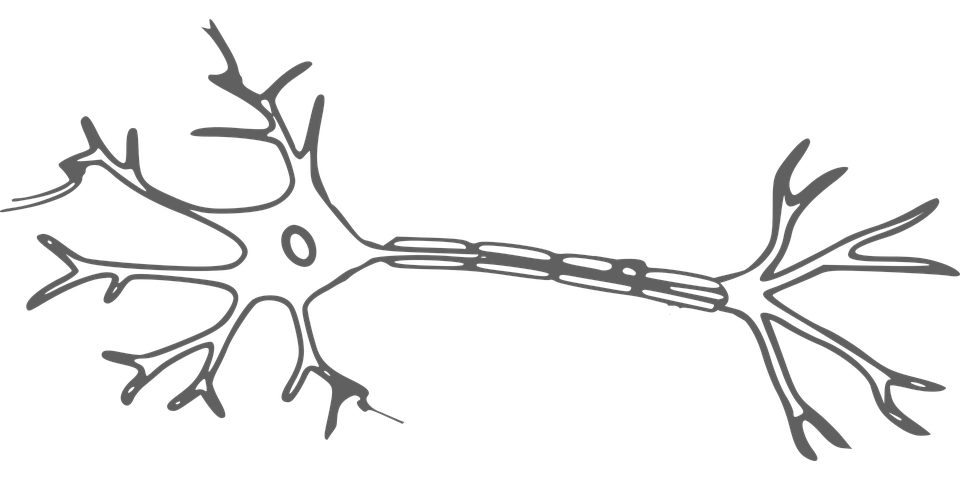
\includegraphics[width=0.8\linewidth]{figures/neuron}
    \caption{Parallelism between a real neuron and the artificial one used in \glspl{mlp}}
    \label{fig:back:neuron}
\end{figure}

Historically, this layer implemented a group of $m$ \emph{perceptrons}.
The perceptron~\cite{rosenblatt1958perceptron} is a biologically-inspired building block for artificial neural networks that has been developed mimicking the structure of biological neurons (see \ref{fig:back:neuron}).
As a neuron cell, it is composed by $n$ inputs $\x_i$ ($i=1 \dots n$), usually connected to the output of other neurons, and a single output $\mathbf{y}$ (axon).
Each input connection is associated with a weight $\w_i$ ($i=1 \dots n$) expressing how much of the signal coming through that connection is promoted or inhibited.
Weights in a perceptron are interpreted as the strength of the interconnection between neuron cells.
The neuron ``fires'' when the combination of their weighted inputs gets above a certain threshold;
this is modelled in the perceptron defining its output as the activation function $\a(\cdot)$ applied to the inner product between input and weights
%
\begin{equation}
    \y_j = \a \( \sum_{i=1}^n \w_i \x_i + b\) \,,
\end{equation}
%
where $\y_j$ is the output of a particular neuron and $b \in \R$ is an optional weight used as bias term.
% The weight vector $\w$ is tuned in the training phase in order to
A layer composed by $m$ perceptrons (and thus $m$ outputs $\y_j, j=1 \dots m$) sharing the same input $\x$ can be formalized with \ref{eq:back:fully-connected}, where the columns of $\W$ correspond to the weights of the $m$ perceptrons.
% Feed-forward artificial neural networks built stacking layers of perceptrons are called \glspl{mlp}.
In \glspl{mlp}, the outputs of a layer are densely connected to the input of each neuron comprising the next layer, hence the name ``fully-connected layer''.
The output of a \gls{mlp} with $L$ layers is defined as
%
\begin{equation}
    \y = \a \( \W_L \( \dots \a \( \W_2 \( \a \( \W_1 \x + \b_1 \) \) + \b_2 \) \) + \b_L \) \,,
\end{equation}
%
where $\(\W_i, \b_i \)$ are the parameters of the $i$-th fully-connected layer in the network.

\subsubsection{Convolutional Neural Networks}

\begin{figure}
    % TODO [FIG] example of crosscorr on image
    \centering
    \includegraphics[width=0.5\linewidth]{figures/cross-correlation2d}
    \caption{Example of cross-correlation between 2D signals}
    \label{fig:back:2d-cross-corr}
\end{figure}

A \gls{cnn} is a feed-forward artificial neural network composed by at least one \emph{convolutional} layer.
This kind of layer computes the cross-correlation between the input and a set of learnable filters.
Since there is a strong similarity between the convolution and the cross-correlation operations, this layer is often attributed with the adjective ``convolutional'' in the \gls{dl} literature;
thus we will adopt the same terminology throughout this thesis.

\paragraph{Cross-correlation}
The \emph{cross-correlation} (also called \emph{sliding inner product}) is typically used in signal processing to search for matches between two signals.
Intuitively, a small signal called \emph{filter} containing the prototype we want to match is slided on a bigger input signal, and for each position, the inner product between the intersection of the two signals measures the quality of the match.
We will provide the reader with the formulation of the two-dimensional version of the cross-correlation due to its massive adoption in image-related fields that are of interest for this work.

Given a two-dimensional input matrix $\x \in \R^{H \times W}$ and a two-dimensional filter $\w \in \R^{K_1 \times K_2}$, %with $K \ll \min(H,W)$,
the cross-correlation $\y \in \R^{H' \times W'}$ between $\x$ and $\w$ is given by
%
\begin{equation}\label{eq:back:cross-correlation}
    \y_{u,v} = \sum_{i=1}^{K_1} \sum_{j=1}^{K_2} \w_{i,j} \x_{i+u-1,j+v-1} \,,
\end{equation}
%
where $u = 1, \dots, H'$ and $v = 1, \dots W'$.
Intuitively, the filter $\w$ is superimposed on the input $\x$, and for each possible position $(u,v)$, the scalar product between the covered input and the filter is computed.
Depending on the presence of padding $P$ added to each side of the input and the stride $S$ of the filter application, the output dimensionality changes following the relations
\begin{equation} \label{eq:back:conv-size}
\begin{split}
    H' = \left \lfloor \frac{H + 2 \times P - K_1}{S} \right \rfloor + 1 \,,\quad
    W' &= \left \lfloor \frac{W + 2 \times P - K_2}{S} \right \rfloor + 1 \,.
\end{split}
\end{equation}
Inputs and outputs of convolutional layers are also called \emph{feature maps}, since high values in the two-dimensional map are usually interpreted as the presence of a feature a particular filter has learnt to identify.
A depiction of 2D cross-correlation is reported in~\ref{fig:back:2d-cross-corr}.

\begin{figure}
    \centering
    \includegraphics[width=\linewidth]{figures/convolution}
    \caption{Depiction of 2D cross-correlation on volumes implemented in convolutional layers}
    \label{fig:back:convolution}
\end{figure}

\paragraph{2D Cross-correlation on Volumes}
\ref{eq:back:cross-correlation} defines the cross-correlation operation for inputs and outputs having both a single feature map.
Images instead are represented as 3-D tensors having $C$ channels (e.g. $C=3$ for RGB data, $C=1$ for grayscale) and two spatial dimensions $H$ and $W$;
thus, the definition of the 2D cross-correlation is extended to 3D tensors letting the filters span the depth of the input tensor.
In such way, filters are still applied over the two spatial dimensions $H$ and $W$, but each output value depends on all the input feature maps in a particular spatial position.
Formally, given an input tensor $\x \in \R^{H \times W \times C}$ and a filter $\w \in \R^{K_1 \times K_2 \times C}$ the cross-correlation $\y \in \R^{H' \times W'}$ between $\x$ and $\w$ is defined as
%
\begin{equation}\label{eq:back:channel-cross-correlation}
    \y_{u,v} = \sum_{i=1}^{K_1} \sum_{j=1}^{K_2} \sum_{k=1}^C \w_{i,j,k} \x_{i+u-1,j+v-1,k} \,.
\end{equation}

A convolution layer is often composed by a bank of $K$ filters.
Each filter is applied to the input, obtaining $K$ output feature maps that are stacked along the depth dimension.
The obtained output is a new 3D tensor $\y \in \R^{H' \times W' \times K}$ that is commonly followed by an element-wise non-linear activation $\a(\cdot)$.
The entire process is depicted in \ref{fig:back:convolution}.

The main difference between fully-connected layers and convolutional layers is the way weights are utilized;
while fully-connected layers have a dedicated weight for each couple of input and output features, a convolutional layer shares the weights of its filters across the spatial dimensions, thus learning to detect translation-invariant features by design.

\paragraph{Pooling Layers}
Pooling layers are often used in \glspl{cnn} to reduce the amount of data to be processed in the next layers.
As the name suggests, this kind of layers pools data in groups and aggregates them using a non-parametric aggregation function, such as maximum or average.
The groups are defined as fixed-size windows that are slided along one or more dimensions of the data in the same way the cross-correlation operator is applied.
In the two-dimensional case, input and output sizes follow \ref{eq:back:conv-size}.
The application of convolutional layers having small strides usually produce redundant local information in their output.
Thus, a max-pooling layer is often used to reduce the resolution of intermediate feature maps.
% Instead, sum- and average-pooling are used to produce

\paragraph{Features hierarchy in \glspl{cnn}}
Convolutional layers are stacked to build deep \glspl{cnn}, that are the one of the core tools of Deep Learning for image perception and analysis~\cite{krizhevsky2012imagenet,sermanet2013overfeat,simonyan2014very,he2015delving,he2016deep,xie2017aggregated}.
Once trained, filters in a deep \gls{cnn} tend to organize in a hierarchy of detectors, where layers near the input detect the presence of simple features in the input data, while the following layers build up from them and detect more complex features.
A successful example of the representative power of \glspl{cnn} is object recognition.
% TODO [CITE] object hierarchical decomposition
The visual aspect of objects in images follow a hierarchical organization: an object can be decomposed in parts, parts in patches, patches in textures, textures in edges or blobs, and finally in pixels~\cite{}.
\begin{figure}
    % TODO [KEEP?] is feat hier figure valuable?
    \centering
    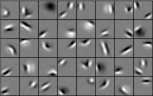
\includegraphics[height=2.9cm]{img/feat-hier-1.png}%
    \hfill%
    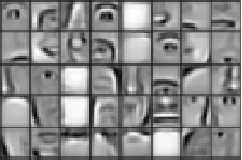
\includegraphics[height=2.9cm]{img/feat-hier-2.png}%
    \hfill%
    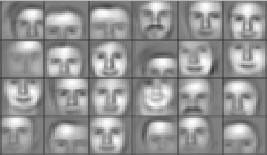
\includegraphics[height=2.9cm]{img/feat-hier-3.png}%
    \newline
    \caption{
    Visualization of the feature hierarchy learned by convolutional layers in a \gls{dl}-model trained on faces.
    Low-level features (edges and blobs, on the left) are detected and then combined to recognize parts (eyes, nose, mouth, in the middle) and finally faces (on the right).
    \figfrom{lee2011unsupervised}
    }
    \label{fig:back:filter-hier}
\end{figure}
\Glspl{cnn} trained to recognize objects, directly or indirectly, often organize their hierarchy of detectors following this kind of visual decomposition of objects (see \ref{fig:back:filter-hier}).


\subsection{Recurrent Neural Networks}
\label{subsec:back:rnn}

A \acrfull{rnn} is a stateful artificial neural network with feedback connections in which the output depends not only on the input, but also on the current state of the network~\cite{goodfellow2016deep,rumelhart1986learning}.
The state of the network acts as a memory which is updated at each input, allowing information to persist between inputs.
This architecture is naturally able to process sequences of inputs;
the elements of a sequence can be fed to the network one by one, updating the internal state of the network to compactly represent the sequence processed so far regardless of its length.
% This is achieved by adding a cycle in the computation graph --

\begin{figure}
    \centering
    \includegraphics[width=.9\linewidth]{figures/rnn}
    \caption{Basic architecture of a \acrlong{rnn} (left). On the right, its unrolled version for a sequence of length 5.}
    \label{fig:back:rnn}
\end{figure}

Given a sequence of inputs of length $T$ $\x_t \in \R^n, t = 1 \dots T$, and an initial state $\h_0 \in \R^m$, a \gls{rnn} can be described as a parametric function mapping the input and the state at a certain timestep to the next hidden state
%
\begin{equation}\label{eq:back:rnn}
    \h_t = f\(\x_t, \h_{t-1}; \W\) \,,
\end{equation}
%
where $f(\cdot)$ is the \emph{recurrent cell} of the \gls{rnn} parametrized by the weights $\W$, and $\h_t \in \R^m, t = 1 \dots T$ is the hidden state at timestep $t$, i.e.\ the state of the network after all inputs until $\x_t$ have been processed.
In its simplest form, the recurrent cell $f$ can be implemented using a fully-connected layer that operates
on the concatenation of the current state and input
%
\begin{equation}
    \h_t = \W [ \x_t | \h_{t-1} ] + \b \,,
\end{equation}
%
where $\W$ and $\b$ are the parameters of a fully-connected layer, and $[\cdot|\cdot]$ is the concatenation operation.
During learning, the \gls{rnn} is unrolled in time to the length of the input sequence to create an acyclic computation graph similar to \glspl{ffnn} (see \ref{fig:back:rnn}) on which standard training procedures can be applied (that will be discussed in \ref{subsec:back:optim}).
Depending on the task we want to model, we could be interested in the last hidden state $\h_T$ compactly represent the whole sequence, or we could use a combination of all hidden states $\h_i, i=1 \dots T$ to get access to the evolution of the information processed through time.

\paragraph{Bidirectional \glspl{rnn}}
In many tasks -- such as sequence classification and segmentation -- also the future context of the sequence is informative. However, \ref{eq:back:rnn} defines a \gls{rnn} encoding only past information, i.e.\   $\h_t$ depends only on information at time step $t' < t$.
To overcome this limitation, \emph{bidirectional} \glspl{rnn} have been proposed~\cite{schuster1997bidirectional}.
Bidirectional architectures adds a separate recurrent cell which process the sequence in reverse order (from future to past)
%
\begin{equation}
    \h'_t = f'\(\x_t, \h'_{t+1}; \W'\) \,,
\end{equation}
%
where $\h'_t$ encodes the "future" part of the sequence, i.e.\ depends on information at time step $t' > t$.
The concatenation of the internal states of both past-to-future and future-to-past \glspl{rnn} $[\h_t | \h'_t]$ is often used as the representation of the whole sequence.

\begin{figure}
    \centering
    \includegraphics[width=.9\linewidth]{figures/bidir-rnn}
    \caption{Unrolled version of a Bidirectional \gls{rnn} for a sequence of length 5}
    \label{fig:back:bidir-rnn}
\end{figure}

\subsubsection{Long Short-Term Memory}

\Gls{lstm}~\cite{hochreiter1997long} is a type of \gls{rnn} with a special formulation of the recurrent cell that has proved its effectiveness in several sequence-modeling tasks~\cite{graves2013speech,sutskever2014sequence,donahue2015long,vinyals2015show}.
This particular formulation is aimed at solving some major drawbacks of vanilla \glspl{rnn}, most importantly the inability to encode long-term dependencies in long sequences due to gradient instability problems, namely the problem of vanishing or exploding gradients ~\cite{pascanu2013difficulty}.
\Gls{lstm} cells are comprised by four learnable gating functions that better control the evolution of the internal state of the cell when dealing with long sequences, and mitigating problems occurring in vanilla RNNs, such as vanishing gradients~\cite{bayer2015learning}.

Let $\x_t \in \R^n$ an element of a sequence, and $\h_{t-1} \in \R^m$ the current hidden state.
The \emph{forget} gate $\f_t$ decides which information is to be discarded at the current step, and it is implemented as a fully-connected layer with $p$ output features and parameters $\w_f \in \R^{(n+m)\times p}, \b_f \in \R^p$ followed by a sigmoid activation
\begin{equation*}
    \f_t = \sigma\(\w_f [\h_{t-1} | \x_t] + \b_f\) \,.
\end{equation*}
The input gate $\i_t$ encodes the information that need to be inserted in the internal state of the cell $\c_t$, and it is implemented following the same rationale of the previous gate
\begin{equation*}
    \i_t = \sigma\(\w_i [\h_{t-1} | \x_t] + \b_i\) \,.
\end{equation*}
The update gate $\u_t$ modulates the amount of new input to be inserted in the internal state of the cell $\c_t$
\begin{equation*}
    \u_t = \tanh\(\w_u [\h_{t-1} | \x_t] + \b_u\) \,.
\end{equation*}
The new cell state $\c_t \in \R^p$ is computed as the sum of two terms;
the first one, given by the element-wise product ($*$) between the forget gate and the previous cell state, represents the part of the old state not to be forgotten;
the second one, computed as the element-wise product of the input and update gates, represent the modulated input to be kept in the new state;
\begin{equation*}
    \c_t = \f_t * \c_{t-1} + \i_t * \u_t \,.
\end{equation*}
The output gate $\o_t$ decides which information in the cell needs to be transferred to the final state $\h_t$
\begin{equation*}
    \o_t = \sigma\(\w_o [\h_{t-1} | \x_t] + \b_o\) \,,
\end{equation*}
and finally, the output state $\h_t$ is computed as
\begin{equation*}
    \h_t = \o_t * \tanh\(\c_t\) \,.
\end{equation*}
%
With an abuse of notation, the complete \gls{lstm} formulation can be compactly written as follows:

%\begin{align}\label{eq:back:lstm}
    % \begin{pmatrix} \i_t\\ \f_t \\ \o_t \\ \u_t \end{pmatrix}
%    \i_t &= \sigma\(\W_i [\h_{t-1} | \x_t] + \b_i\) \\
%    \f_t &= \sigma\(\W_f [\h_{t-1} | \x_t] + \b_f\) \\
%    \o_t &= \sigma\(\W_o [\h_{t-1} | \x_t] + \b_o\) \\
%    \u_t &= \tanh\(\W_u [\h_{t-1} | \x_t] + \b_u\) \\[2ex]
%    \c_t &= \f_t * \c_{t-1} + \i_t * \u_t \\
%    \h_t &= \o_t * \tanh\(\c_t\)
%\end{align}
\begin{align}\label{eq:back:lstm}
\begin{aligned}
    \begin{pmatrix} \i_t\\ \f_t \\ \o_t \\ \u_t \end{pmatrix} &=
    \begin{pmatrix} \sigma \\ \sigma \\ \sigma \\ \tanh \end{pmatrix}
    \( \W \begin{pmatrix} \x_t \\ \h_{t-1} \end{pmatrix} \) \\[2ex]
    \c_t &= \f_t * \c_{t-1} + \i_t * \u_t \\
    \h_t &= \o_t * \tanh\(\c_t\) \,,
\end{aligned}
\end{align}
%
where $\W \in \R^{(n+m) \times 4p}$ summarizes all the parameters of all the fully-connected layers forming the gates.
% TODO: [FIG] lstm?
A depiction of the \gls{lstm} cell is aslo available in \ref{fig:back:lstm}.

\begin{figure}
    \centering
    \includegraphics[width=\linewidth]{figures/lstm}
    \caption{Example of \gls{lstm} cell}
    \label{fig:back:lstm}
\end{figure}

\subsection{Loss Functions}
\label{subsec:back:loss}

Loss functions are a key component of \gls{ml} methods.
Its role is to quantitatively assign a value of goodness to a model in reference to the particular task we want to solve.

Given a training set $\X = \{\(\x_i, \y^\star_i\),\; i=1,\dots,N\}$ comprised by $N$ couples of inputs and desired outputs, the quality of a particular setting of parameters $\Theta$ is quantitatively defined by a \emph{loss function} $\L\(\X; \Theta\)$ that measures how much predictions and targets differ.
A loss function is usually defined as one of more terms summed together.
The main term $\L_d\(\X; \Theta\)$ is defined as the average of the individual loss values computed on each sample of the dataset $\L\(\y_i, \y^\star_i\)$ -- we denote it the \emph{data term}.
A secondary optional term $\L_r(\Theta)$ is often used to regularize the network and depends only on the model parameters $\Theta$ -- we indicate this as \emph{regularization term}.
Regularization consists of model constraints added to avoid other undesired properties during training such as \emph{overfitting} -- i.e. the tendency of a model to predict well known data while failing to make correct prediction for unseen data.
Regularization has gained importance in the \gls{dl} field due to the huge amount of parameters models are usually comprised of, thus increasing the risk of overfit on the train data.
The regularization term is usually multiplied by a hyperparameter $\alpha$ and then added to the loss function.
A general formulation of the loss function is
%
\begin{equation} \label{eq:back:loss}
\begin{aligned}
    \L\(\X; \Theta\) &= \overbrace{\L_d\(\X; \Theta\)}^{\textrm{data term}}&+\, \alpha &\overbrace{\L_r\(\Theta\)}^{\textrm{regularization term}}\\
                     &= \frac{1}{N} \sum_{i=1}^N \L\(\y_i, \y^\star_i\)&+\alpha & \,\quad \L_r\(\Theta\) \\
                     &= \frac{1}{N} \sum_{i=1}^N \L\(f\(\x_i; \Theta\), \y^\star_i\)&+\alpha & \,\quad\L_r\(\Theta\) \,.
\end{aligned}
\end{equation}
%
%where the optimal value of $\alpha depends on the absolute values of the loss terms and

In the next paragraphs, we will provide the reader with some of the most used formulations of $\L\(\y_i, \y^\star_i\)$ and $\L_r(\Theta)$ of interest for this work.

\paragraph{Mean Squared Error Loss}
When dealing with regression problems, we want our predictions to be close to the one or more real-valued targets.
For example, in an age estimation problem, we want our network to predict the exact age expressed as a real value, e.g. $46,5$.
The mean squared error between predictions $\z$ and targets $\z^\star$ is a commonly used loss function to measure the goodness of regressions
\begin{equation} \label{eq:back:mse}
    \L_\textrm{MSE}(\z, \z^\star) = \frac{1}{2} \( \z - \z^\star \)^2 \,.
\end{equation}
%
The scale factor $\frac{1}{2}$ is usually introduced to simplify the gradient computation when using this loss function (more details on this in \ref{subsec:back:optim}).

\paragraph{Cross-entropy Loss}
The cross-entropy loss is commonly used in \gls{ml} to measure the distance between two categorical distributions.
It is commonly adopted in single-label classification tasks, where a single label have to be assigned to a piece of data choosing from $N$ labels ($N \geq 2$).
Let $\z$ and $\z^\star$ the probability masses of two $N$-way categorical distributions, i.e. $\z_i, \z^\star_i \in [0,1],\; \sum_{i=1}^N \z_i = 1, \sum_{i=1}^N \z^\star_i = 1$;
the cross-entropy loss between the predicted distribution $\z$ and the target one $\z^\star$ is defined as
%
\begin{equation} \label{eq:back:cross-entropy}
    \L_\textrm{CE}(\z, \z^\star) = - \sum_{i=1}^N \z^\star_i \log \z_i \,.
\end{equation}
%
Classification models are often designed to output a $N$-dimensional vector $\z$ that is mapped to a categorical distribution via the \emph{softmax} function
%
\begin{equation} \label{eq:back:softmax}
    \textrm{softmax}(\z)_i = \frac{e^{\z_i}}{\sum_{j=1}^N e^{\z_j}} \,.
\end{equation}

\paragraph{$\mathbf{L_p}$ Weight Decay}
The most used regulatization terms in the \gls{dl} literature are the ones penalizing the parameters having large norm.
This is usually implemented defining the regularization term $\L_r\(\Theta\)$ added to the loss to be minimized as the $p$-norm of the parameters.
Practical definitions have been adopted for $p=2$ ($\mathbf{L_2}$ weight decay) and for $p=1$ ($\mathbf{L_1}$ weight decay).
The former produces a more uniform utilization of all the available parameters, penalizing under-utilized and over-utilized weights~\cite{ng2004feature}, and is defined as
%
\begin{equation} \label{eq:back:l2-weight-decay}
    \L_r\(\Theta\) = \frac{1}{2} ||\Theta||_2^2 = \frac{1}{2} \sum_i \theta_i^2 \,.
\end{equation}
%
The latter instead tends to produce a more sparse weight configuration, i.e. with many parameters having a null optimal value~\cite{ng2004feature}, and is defined as
%
\begin{equation} \label{eq:back:l1-weight-decay}
    \L_r\(\Theta\) = ||\Theta||_1 = \sum_i |\theta_i| \,.
\end{equation}

\subsection{Gradient-Based Optimization}
\label{subsec:back:optim}

As already stated, solutions of \ref{eq:back:optim} are the parameter configurations $\Theta$ that minimizes the loss function $\L$ defined over a given training set $\X$.
Unfortunately, in very rare cases closed-form solutions of \ref{eq:back:optim} are available for practical formulations of \gls{dl} models $f(\cdot)$ due to the non-linear non-convex nature of deep models.
In the past years, there was reluctance in the \gls{ml} field to work with non-convex models due to the lack of theoretical guarantees on their convergence.
Nevertheless, recent developments shown that non-convex model -- albeit having less guarantees -- have higher capacity and representational power and thus have a better overall performance~\cite{bengio2007scaling}.
The most common approach to find suboptimal (but valuable) solutions to \ref{eq:back:optim} is using iterative gradient-based optimization.

\paragraph{Gradient Descent}
In gradient-based optimization, given a training set $\X$ and a parameter configuration $\Theta$, we search for a new solution following the direction of the gradient of the loss function $\nabla\L\(\X, \Theta\)$ with respect to the parameters $\Theta$.
The direction given by $\nabla\L\(\X, \Theta\)$ is the one of maximum steepness of the loss surface in the parameter space, that is, the one that maximize the loss change locally.
A new parameter configuration $\Theta^\star$ is chosen \emph{descending} the loss surface along the direction of maximum steepness with a step size of $\lambda$, that is
%
\begin{equation} \label{eq:back:gradient-descent}
    \Theta^\star = \Theta - \lambda \nabla\L\(\X, \Theta\) \,.
\end{equation}
%
This update rule can be iterated until a (local or global) minimum of the loss function is reached.
This procedure is called \emph{gradient descent} optimization, and in the \gls{ml} field $\lambda$ is referred to as the \emph{learning rate}.
\begin{figure}
    \centering
    \includegraphics[width=\linewidth]{figures/gradient-descent}
    \caption{Example of gradient descent optimization on a loss surface $\L(\X)$ defined over a 2D parameter space $(\w_1, \w_2)$ with two different starting points}
    \label{fig:back:gradient-descent}
\end{figure}
A depiction of this algorithm for a 2D toy example is reported in \ref{fig:back:gradient-descent}.
Bigger learning rates correspond to bigger steps along the loss surface that usually improve the convergence rate and avoid local minima at the cost of a higher risk of oscillating around minimum points.
Small learning rates, instead, bring a lower convergence rate but are able to better exploit the local topology of the loss function, reaching a locally better solution.

\paragraph{Back-propagation}
As formalized in \ref{eq:back:deepnet}, \glspl{dnn} are comprised by many composition of non-linear functions $f_i$ each having its own set of parameters $\theta_i$.
Thus, to perform gradient descent on \gls{dl} models, we need to compute gradients $\nabla\L\(\X, \theta_i\)$ for each $\theta_i \in \Theta$.
This is efficiently done by \emph{back-propagation}~\cite{rumelhart1986learning,lecun1988theoretical}.

In back-propagation, we start computing the gradient of the loss function from the last layer (the one that produce the final predictions), and we propagate the error backwards to previous layers using the chain-rule for computing derivatives of compound functions.
For simplicity, we report the formulation of back-propagation for a \acrfull{ffnn}, but this mechanism is general and applies to all differentiable architectures.
Let $f(\x;\Theta)$ a \gls{ffnn} composed by $L$ layers with parameters $\Theta = \{\theta_1, \dots, \theta_L\}$ defined in \ref{eq:back:deepnet}, and let $\o_i$ the output of the $i$-th layer
\begin{equation}
\begin{split}
\o_0 &= \x \\
\o_i &= f_i \(\o_{i-1}; \theta_i \) \,.
\end{split}
\end{equation}
The gradient $\frac{\partial \L}{\partial \theta_i}$ of the loss function $\L$ with respect to $\theta_i$ can be decomposed using the chain-rule as
\begin{equation}
\begin{split}
    \frac{\partial \L}{\partial \theta_i} &= \frac{\partial \L}{\partial \o_i} \cdot \frac{\partial \o_i}{\partial \theta_i} \\
                                          &= \frac{\partial \L}{\partial \o_L} \cdot \frac{\partial \o_L}{\partial \o_{L-1}} \cdots  \frac{\partial \o_{i+1}}{\partial \o_i} \cdot \frac{\partial \o_i}{\partial \theta_i} \,,
\end{split}
\end{equation}
%
where the partial derivatives $\frac{\partial \o_{i+1}}{\partial \o_i}$ and $\frac{\partial \o_i}{\partial \theta_i}$ are well defined and depend on the implementation of the $i$-th layer $f_i$.
The formulations of the loss function $\L$ and intermediate layers $f_i$ are chosen to be differentiable to ensure that also the entire model -- being a composition of differentiable functions -- is in turn differentiable, and that back-propagation can be applied to efficiently compute gradients.


\paragraph{Stochastic Gradient Descent}
In our presentation of gradient-based optimization so far, the computation of the loss function $\L\(\X; \Theta\)$ and its gradient depend on the whole dataset $\X$.
This may be limiting for \gls{dl} applications where very large training sets are needed to train models, thus increasing the computational cost needed to compute the exact value of $\L\(\X; \Theta\)$.
To overcome this problem, \gls{sgd} and in particular mini-batch \gls{sgd}~\cite{rumelhart1986learning} have been proposed to compute an estimate the loss function and its gradients at a lower computational cost.

In mini-batch \gls{sgd}, we use a small random sample of the entire training set $ \tilde{\X} = \{ (\tilde{\x_i}, \tilde{\y_i}), i = 1 \dots B \} \subset \X$ (called \emph{batch} or \emph{mini-batch}) to compute an estimate of loss function
\begin{equation} \label{eq:back:minibatch-sgd}
\tilde{\L} \(\X; \Theta\) = \L (\tilde{\X}; \Theta) = \frac{1}{B} \sum_{i=1}^B \L(f(\tilde{\x_i}; \Theta), \tilde{\y_i}) \,,
\end{equation}
which in turn is used in back-propagation to estimate its gradient $\nabla \L(\tilde{\X}; \Theta)$ and perform the parameter update as specified in \ref{eq:back:gradient-descent}.
The size of the mini-batch size $B$ is a hyperparameter that controls the trade-off between the computational cost needed to compute the loss and the quality of the loss estimate.

\paragraph{\gls{sgd} with Momentum}
A successful proposal to improve the parameter update rule presented in \ref{eq:back:gradient-descent} is \gls{sgd} with \emph{momentum}~\cite{qian1999momentum}.
The key idea of momentum is to add to the current direction given by the loss gradient a fraction of the direction computed in the previous iteration, such that the direction we are following to descend the loss surface gains inertia and smooths out eventual oscillations given by very steep loss manifolds.
Given $\m^{(k-1)}$ the direction of the previous iteration, we define the new direction to follow $\m^{(k)}$ as
\begin{equation} \label{eq:back:momentum}
\begin{aligned}
    \m^{(0)} &= 0 \\
    \m^{(k)} &= \gamma \m^{(k-1)} + \nabla\L\(\X; \Theta^{(k)}\) \\
    \Theta^{(k+1)} &= \Theta^{(k)} - \lambda \m^{(k)} \,,
\end{aligned}
\end{equation}
%
where $\gamma \in (0,1)$ is the momentum of the previous direction.
Commonly used values for $\gamma$ are around $0.9$.
A good analogy to comprehend the rationale behind momentum is a ball pushed down a hill:
the higher the momentum $\gamma$, the more inertia the ball has, and the less it is influenced by steepness variations during the descent.
This modified update rule tends to discard the oscillating directions of the gradient while strengthening the stable directions over iterations;
this brings a reduction of oscillations while descending the loss manifold and thus a faster convergence.

\paragraph{Adam}
Another widely used parameter update rule in the \gls{dl} literature is \gls{adam}~\cite{kingma2014adam}.
Similar to other proposed update rules (such as Adagrad~\cite{duchi2011adaptive} or Adadelta~\cite{zeiler2012adadelta}), this method computes an adaptive learning rate for each parameter to be optimized based on the second moment of the gradients $\v$ (i.e. squared gradients), but in addition, it also estimates the first moment $\m$ (the mean of the gradient itself) as in \gls{sgd} with momentum
%
\begin{equation} \label{eq:back:adam-moments}
\begin{aligned}
    \m^{(k)} &= \beta_1  \m^{(k-1)} + \(1 - \beta_1 \)  \nabla\L\(\X; \Theta^{(k)}\) \\
    \v^{(k)} &= \beta_2  \v^{(k-1)} + \(1 - \beta_2 \)  \nabla\L\(\X; \Theta^{(k)}\)^2 \,.
\end{aligned}
\end{equation}
%
The hyperparameters $\beta_1$ and $\beta_2$ are respectively controlling the aggressiveness of the exponential average of the two moments $m^{(k)}$ and $v^{(k)}$.
Since the initial values of the moments are initialized to zero, the authors propose to use the bias-corrected version of the moments, that is
%
\begin{equation} \label{eq:back:adam-moments-bias}
\begin{aligned}
    \hat{\m}^{(k)} &= \frac{\m^{(k)}}{1 - \beta_1^k} \\
    \hat{\v}^{(k)} &= \frac{\v^{(k)}}{1 - \beta_2^k} \,.
\end{aligned}
\end{equation}
%
Finally, moments estimates are used to formulate the \gls{adam} update rule
%
\begin{equation} \label{eq:back:adam}
\theta^{(k+1)}_i &= \theta^{(k)}_i - \frac{\lambda}{\sqrt{\hat{\v}^{(k)}_i} + \epsilon} \m^{(k)}_i \qquad \forall \theta_i \in \Theta \,,
\end{equation}
%
where $\m^{(k)}_i$ and $\hat{\v}^{(k)}_i$ are the first and second moments estimates of the gradients corresponding to parameter $\theta_i$, and $\epsilon$ is a small values to prevent division by zero.
Commonly used values for hyperparameters are $\beta_1 = 0.9$, $\beta_2 = 0.999$, and $\epsilon = 10^{-8}$, as suggested by the authors.


% TODO move dropout?
\paragraph{Dropout}
Regularization is not limited to regularization loss terms only.
\emph{Dropout}~\cite{hinton2012improving} is a common regularization technique for \glspl{dnn} which consists in deactivatating (drop) some neurons of an internal layer (by setting their activations to zero) during the training phase and thus enabling the back-propagation of the error only in the survived neurons.
The choice of the neurons to deactivate is random: each neuron on which dropout is applied has a given probability $p$ to survive.
The employment of this technique usually increases the number of training iterations needed to a model to converge, because only the subset of weights of the survived neuron are updated in an optimization step.
However, training a random subset of neurons at each iteration reduces the co-adaptation of neurons, which tend to learn a more diversified and independent configurations of weights.
This results in a increased ability of bigger models to exploit their capacity and limit overfit.
At test time, all neurons are used, virtually exploiting and combining the predictions of many independently trained models.
The activations of the layers trained with dropout are scaled by $p$ to approximate the combined prediction produced by the virtual ensemble of sub-networks.


\section{Image Classification}
\label{sec:back:image-classification}

% TODO intro to img classification, examples and applications
% Examples (simple classif., sentiment analysis, etc.)
% Classifying images is super cool bla bla
In this section, we formally define the problem of image classification, and we analyze and review recent solutions based on \acrlong{dl} -- in particular Deep \acrlongpl{cnn} -- proposed in the literature.

% TODO sentence dropped here at random
In the case of image classification, the data on which classifiers must rely on is raw pixel data, usually organized in a tensor with shape $(H, W, C)$, respectively representing the height, the width, and the number of channels of the image.

Many real-world problems in image understanding, such as object and face recognition, anomaly detection, and ..., can be formalized as classification problems.
For this reason, classification methods for images have received an increasing attention in the last decade.

\subsection{Problem Setting}
\label{subsec:back:classification}
Image classification consists of assigning one or more labels to an image $\x$ choosing from a finite set of $L$ labels.
We refer to \emph{single-label} $L$-way classification if only one label has to be picked among the $L$ available, referring to the special case in which $L=2$ as \emph{binary} classification.
If multiple labels can be assigned to a piece of data, we talk about \emph{multi-label} classification.
A multi-label $L$-way classification problem is often decomposed in $L$ independent binary classification sub-problems, each of them focusing on predicting the presence or the absence of one of the available $L$ labels.

Let $I$ the image space;
given an image to be classified $\x \in I$, a single-label $L$-way classifier is a function $f$ mapping $\x$ into the label space.
% Solving a classification problem reduces to find a suitable classifier $f$ that agrees with observed data labels.
The commonly used form of classification is \emph{probabilistic}, in the sense that soft assignments to the available labels are considered instead of hard ones.
In this case, an image $\x$ is mapped into its posterior probability $p_i = p(\y = i | \x)$ of belonging to category $i$, for each category $i \in \{1, \dots, L\}$.
Thus, the classifier is a function $f: I \to \p$ which maps an image to the parameters $\p = (p_1, \ldots, p_L), \sum_{i=1}^L p_i = 1$ of a categorical distribution defined over the label space.
Soft assignments present a broad range of advantages with respect to hard assignments, the most important one being differentiability, which enables and facilitates gradient-based learning of models for $f$.

% TODO expand image classification problem setting?

\subsection{Evaluation}
\label{subsec:back:classif-eval}

In this section, we will report the most commonly used evaluation metrics to measure the quality of classification models.
Assume $\Y = (y_1, \ldots, y_n)$ is a set of predictions and $\tilde{\Y} = (\tilde{y}_1, \ldots, \tilde{y}_n)$ the set of the ground-truth labels for a single-label $L$-way classification problem, with $y_i, \tilde{y}_i \in \{1, \ldots, L\}$. % for $i \in \{1, \ldots, N\}$.

\paragraph{Confusion Matrix}
One of the fundamental tools for evaluating a set of label assignments is the \emph{confusion matrix} $C = \{c_{ij}\}$, which compactly reports the co-occurence of predicted and ground-truth labels.
The element $c_{ij}$ of the matrix indicates the number of times the model predicted the class $i$ for a sample belonging to class $j$.
We report in \ref{tab:back:confusion} the confusion matrix for the binary case ($L=2$) together with the terminology used to refer to particular values in the matrix.
For the binary case, many useful metrics can be computed from the confusion matrix, and we will introduce some of them in the next paragraphs.
Notice that the same metrics can be applied to cases with $L > 2$ by reformulating them as $L$ binary problems, where one class is the positive class, and the other $(L-1)$ are condensed in the negative class;
metrics can be computed considering each class as the positive one and then aggregated to obtain a global metric for the classification.

\begin{table}
\newcolumntype{M}[1]{>{\centering\arraybackslash}m{#1}}
\renewcommand{\arraystretch}{1.5}

\begin{tabularx}{\linewidth}{cr|M{1.3cm}|M{1.3cm}|>{\hskip 2cm}r@{\hskip 3pt}X}
\multicolumn{4}{c}{}                                                                                                                                      & $\mathrm{TP}=$ & True Positives, i.e. correct hits           \\
\multicolumn{2}{c}{}                                                  & \multicolumn{2}{c}{\bfseries Actual class}                                        & $\mathrm{TN}=$ & True Negatives, i.e. correct rejections     \\
\multicolumn{2}{c}{}                                                  & \multicolumn{1}{c}{\itshape \small Positive} & \multicolumn{1}{c}{\itshape \small Negative} & $\mathrm{FP}=$ & False Positives, i.e. false alarms          \\ \cline{3-4}
\parbox[t]{2mm}{\multirow{2}{*}{\rotatebox[origin=c]{90}{\bfseries Predicted}}} & {\itshape \small Positive} & $\mathrm{TP}$ & $\mathrm{FP}$                   & $\mathrm{FN}=$ & False Negatives, i.e. misses                \\ \cline{3-4}
                                                                      & {\itshape \small Negative}           & $\mathrm{FN}$ & $\mathrm{TN}$                   &  $\mathrm{P}=$ & $\mathrm{TP}+\mathrm{FN}=$ Positive samples \\ \cline{3-4}
\multicolumn{4}{c}{}                                                                                                                                      &  $\mathrm{N}=$ & $\mathrm{TN}+\mathrm{FP}=$ Negative samples \\
\end{tabularx}

\caption{Confusion matrix for a binary classification problem and the related terminology}
\label{tab:back:confusion}
\end{table}

% Accuracy
\paragraph{Accuracy} The accuracy of a classification is defined for the binary case as
\begin{equation} \label{eq:back:accuracy-binary}
    \mathrm{Acc.} = \frac{\mathrm{TP} + \mathrm{TN}}{\mathrm{P} + \mathrm{N}} = \frac{\mathrm{TP} + \mathrm{TN}}{\mathrm{TP} + \mathrm{FN} + \mathrm{TN} + \mathrm{FP}} \,,
\end{equation}
that is the fraction of correctly classified samples.
For the general case with more than two classes, the accuracy is given by the sum of the elements on the diagonal of the confusion matrix -- which contains the counts for correct predictions -- and the total number of classified samples
\begin{equation} \label{eq:back:accuracy}
    \mathrm{Acc.} = \frac{\sum_{i=1}^L c_{ii}}{|Y|} \,.
\end{equation}

% Top-K Accuracy
\paragraph{Top-$K$ Accuracy}
A common variant of the accuracy often used for probabilistic classifiers when many classes are considered, is the \emph{Top-$K$ Accuracy}.
Given the $L$ probabilities (or scores) assigned to a sample by a probabilistic classifier, we consider the prediction correct if the ground-truth class appears in the first $K$ highest scored classes.
The metric then is computed as the fraction of correct predictions.

The accuracy metric is a very simple and intuitive metric for evaluating classifiers, but it may be misleading when employed on unbalanced test sets.
Consider for example a binary classification example with 95 positive and 5 negative samples;
A classifier always predicting the positive class (a trivial acceptor) achieves an accuracy of $.95$ while behaving very poorly on negative classes.
In this scenarios, other ratios derived from the classification matrix are used to better characterize the performances of a classifier.

% TPR TNR
\paragraph{\acrshort{tpr} and \acrshort{tnr}}
The \emph{\gls{tpr}} is the ratio between correctly predicted positive samples and the number of actual positive samples
\begin{equation} \label{eq:back:tpr}
    \mathrm{TPR} = \frac{\mathrm{TP}}{\mathrm{P}} = \frac{\mathrm{TP}}{\mathrm{TP} + \mathrm{FN}} \,.
\end{equation}
It is also known as \emph{Recall} of the positive class, as it indicates the fraction of positive samples correctly accepted as positive.
Similarly, the \gls{tnr} represent the same concept applied to the negative class, and it is defined as
\begin{equation} \label{eq:back:tnr}
    \mathrm{TNR} = \frac{\mathrm{TN}}{\mathrm{N}} = \frac{\mathrm{TN}}{\mathrm{TN} + \mathrm{FP}} \,.
\end{equation}

% FNR FPR
\paragraph{\acrshort{fnr} and \acrshort{fpr}}
While \gls{tpr} and \gls{tnr} measure how well a classifier perform on both classes, the \gls{fnr} and \gls{fpr} are complementary measures that indicate instead the faction of classification errors.
Specifically, the \gls{fnr} is defined as the fraction of positive examples wrongly classified as negatives, and it is complementary to the \gls{tpr}
\begin{equation} \label{eq:back:fnr}
    \mathrm{FNR} = \frac{\mathrm{FN}}{\mathrm{P}} = \frac{\mathrm{FN}}{\mathrm{TP} + \mathrm{FN}} = 1 - \mathrm{TPR}\,.
\end{equation}
Similarly, the \gls{fpr} measures the fraction of errors on the negative class
\begin{equation} \label{eq:back:fpr}
    \mathrm{FPR} = \frac{\mathrm{FP}}{\mathrm{N}} = \frac{\mathrm{FP}}{\mathrm{TN} + \mathrm{FP}} = 1 - \mathrm{TNR}\,.
\end{equation}

\paragraph{\acrshort{roc} and \acrshort{auc}}
Probabilistic classifiers produce soft assignments of each sample to the available classes in the form of scores or confidences from which the final hard classification is obtained.
A common way to do so is to use an acceptance threshold, and depending on the choice of the threshold, the performance of the classifier may vary substantially.
A useful tool to evaluate the performance of the classifier in relation to the threshold is the \gls{roc} plot~\cite{fawcett2006introduction}.
Each point on a \gls{roc} plot represents the performance of the classifier for a given threshold $T$, and has as coordinates the \gls{fpr}$(T)$ (on the x-axis) and the \gls{tpr}$(T)$ (on y-axis) obtained by using $T$.
An optimal classifier lies on the top-left point $(0,1)$, while a random-chance classifier lies on the $TPR = FPR$ line.
A \gls{roc} curve for a given classifier is comprised by all the points obtained by varying the threshold.
The curve starts from $(0,0)$ -- that correspond to having the most stringent threshold, thus a trivial rejector classifier -- and ends in $(1,1)$ -- corresponding to the most permissive threshold that results in a trivial acceptor.
\Gls{roc} curves enables a visual comparison of classifiers, since curves lying closer to the optimal $(0,1)$ point are considered better classifiers independently from the particular threshold chosen.
To quantitatively compare classifiers on the \gls{roc} plane, the \gls{auc} is often computed as a unique threshold-independent metric;
the higher the \gls{roc} curve, the closer the \gls{auc} is to $1$ (see \ref{fig:back:roc}).

\begin{figure}
    \centering
    \includegraphics[width=\linewidth]{figures/roc-example}
    \caption{Example of \acrfull{roc} curves for two binary classifiers, and the relation between their corresponding \acrfullpl{auc}. }
    \label{fig:back:roc}
\end{figure}

\paragraph{\acrshort{eer} Accuracy}
Another useful threshold-independent metric which is commonly used to compare classifiers is the \gls{eer} accuracy.
This is the accuracy obtained by choosing the threshold yielding an equal error rate on both positive and negative classes, i.e.
\begin{equation} \label{eq:back:eer-accuracy}
    \mathrm{EER\ Acc.} = \mathrm{Acc}(T) \quad | \quad \mathrm{FPR}(T) = \mathrm{FNR}(T) \,,
\end{equation}
where $\mathrm{Acc}(T)$, $\mathrm{FPR}(T)$, and $\mathrm{FNR}(T)$ indicates respectively the accuracy, the \gls{fpr}, and the \gls{fnr} obtained using $T$ as threshold.
On the \gls{roc} plot, this threshold setting corresponds to the point where the classifier curve intersect the second diagonal of the unit square, i.e. the $\mathrm{TPR} = 1 - \mathrm{FPR}$ line, which is equivalent to $\mathrm{FPR} = \mathrm{FNR}$ by substituting \ref{eq:back:fnr} in \ref{eq:back:eer-accuracy}.

\subsection{Relevant works}
\label{subsec:back:classif-relwork}

\paragraph{Before \acrlong{dl}}
% TODO divide f in features and classifier, manually (?)
Traditional approaches to image classification required to manually design the classifier $f(\cdot)$.
% ESWA: The traditional approaches to the classification problem use ad-hoc functions to extract from an image specific features that are considered to be indicative of certain objects.
In particular, hand-crafted features detectors and descriptors -- such as SIFT~\cite{lowe2004distinctive}, SURF~\cite{bay2006surf}, ORB~\cite{rublee2011orb}, MSER~\cite{matas2004robust}, KAZE~\cite{alcantarilla2012kaze} to cite some -- were employed to extract information from the image considered indicative for the presence of certain objects.
For example, the presence of features like hard corners and straight edges might indicate man-made objects in the image~\cite{piccinini2012real}.
Shallow classifiers based on \gls{ml} methods -- such as logistic regressors~\cite{mensink2012metric} or \glspl{svm}~\cite{arandjelovic2012three} -- then relied on these extracted features and their aggregation (VLAD~\cite{jegou2010aggregating}, Fisher Vectors~\cite{perronnin2010improving}) to determine which label to be assigned to the image.

% ESWA: it is hard to think of general, robust, reliable features, which map to specific object types; - it is a huge task to find the right combination; - of features for every type of object to classify; - it is difficult to design functions that are robust to translations, rotations and scaling of objects in the image
% ESWA: All these problems make developing high accuracy object detectors and classifiers for a broad range of objects very hard.
However, manually engineered solutions are feasible for very specific problems -- such as image stitching~\cite{brown2007automatic} and 3d reconstruction~\cite{schonberger2016structure} -- where the conditions are well known and modelled.
In general, thinking of features that are invariant to transformations, reliable for many types of objects, and robust to noise and other exogenous factors is often very difficult and time-consuming.
% ESWA: it is often very complex to develop robust and reliable feature detectors and descriptors by hand.
% TODO better definition of VSA
As an example, consider the problem of visual sentiment analysis (further discussed in \ref{ch:cross-learning}), which, in a nutshell, consists in detecting the emotions conveyed by images.
Manually defining a good set of features to extract from images to solve this task is a cumbersome process and usually leads to suboptimal solutions.

\paragraph{ImageNet Challenge and the Deep Learning era}

\begin{table}
    \begin{tabularx}{\linewidth}{p{4.5cm}X>{\centering}c}
        \toprule
        \textbf{Team} & \textbf{Image Features} & \textbf{Error} \\
        \midrule
        \emph{LEAR}~\citep{mensink2012metric} \newline {\footnotesize LEAR INRIA Grenoble} \newline {\footnotesize TVPA Xerox Research Centre Europe} & PCA-reduced FV + dense SIFT & 34.5 \\ % -
        \midrule
        \emph{UvA}~\citep{sanchez2011high} % ,scheirer2012multi}
        \newline {\footnotesize University of Amsterdam} & Compressed FV + SIFT & 29.6 \\ % -
        \midrule
        \emph{XRCE}~\citep{akata2014good} \newline {\footnotesize Xerox Research Centre Europe} \newline {\footnotesize LEAR INRIA} & FV / BOV + multi-scale dense SIFT  & 27.1 \\ % -
        \midrule
        \emph{VGG}~\citep{arandjelovic2012three,sanchez2012modeling} \newline {\footnotesize University of Oxford} & SVM on FV + dense rootSIFT + Color statistics & 27.0 \\ % 50.0
        \midrule
        \emph{ISI}~\citep{harada2012graphical} \newline {\footnotesize University of Tokyo, JST PRESTO} & Gaphical Gaussian Vectors + dense SIFT & 26.2 \\% 53.6
        \midrule
        \emph{SuperVision}~\citep{krizhevsky2012imagenet} \newline {\footnotesize University of Toronto} & Trained features (AlexNet \gls{cnn}) & \textbf{16.4} \\ % 34.2
        \bottomrule
    \end{tabularx}
    \caption{ILSVRC12 leaderboard reporting the accuracy (as top-5 error percentage) on the image classification task obtained by the participating teams. Results taken from~\cite{russakovsky2015imagenet}}
    \label{tab:ilsvrc12-results}
\end{table}

% ESWA: The Deep Learning approach, on the other hand, exploits a large number of ground-truth labeled data to discover which features and combinations of features are most discriminative for each class of objects to be recognized, and builds a combined feature extraction and classification model.
On the other hand, \acrlong{dl} approaches rely on large amount of labeled data to automatically discover which features and combination of them are important for the task.
The main advantage of this kind of approach is its general applicability even to large-scale scenarios where thousands of different classes of images have to be recognized.
Recent results in the \gls{ilsvrc} are a striking evidence of the success of \gls{dl} methods in image classification.
\gls{ilsvrc} is an annual challenge in which competitors are asked to recognize generic objects in images and classify them accordingly choosing from a vast label space (in the order of 1,000 labels).
Before \gls{dl} methods were applied in this competition, leading solutions were based on combinations and aggregation of hand-made local features~\cite{harada2012graphical,akata2014good,sanchez2011high,mensink2012metric}.
Interestingly, in the edition of the challenge occurred in 2012, a \gls{dl} method based on \acrlongpl{cnn}~\cite{krizhevsky2012imagenet} outperformed non-\gls{dl} solutions by a large margin ($16.4 \%$ top-5 error vs $26.2 \%$ of the second place, see \ref{tab:ilsvrc12-results}), marking the beginning of the \gls{dl}-era in the computer vision field.
Since then, we experienced an exponential growth of interest by research communities in \gls{dl} technologies.
While the theories and concepts behind \gls{dl} approaches -- such as artificial neural networks and \acrlong{ml} -- were already studied and formalized in the past~\cite{rosenblatt1958perceptron,rumelhart1985learning,lecun1989backpropagation,widrow199030}, in the last years, the combination of different factors has allowed \acrlong{dl} to flourish.
Most importantly, huge amounts of data -- collected and labeled exploiting Web technologies and crowd-sourcing -- provided the supervision needed by very deep models having millions of parameters to properly train, and modern hardware and accelerators -- such as \glspl{gpu} -- provided the computing power needed to speed up training and evaluation procedures.

%ILSVRC winners (Hybrid, VGG, Inception, Residual, ResNeXT, SENets?)
\paragraph{AlexNet}
% Krizhevsky et al., 2012
We start our review of relevant work in image classification right from the method that won the \gls{ilsvrc}'12 challenge, that is the \gls{dcnn} proposed by~\citet{krizhevsky2012imagenet}, also knwon as \emph{AlexNet}.
Inspired by previous work on handwritten digits recognition~\cite{lecun1989backpropagation}, the AlexNet model is composed by a deep convolutional neural network that maps directly RGB data to labels without relying on explicit feature engineering.
It is comprised by 5 convolutional layers with \gls{relu} activation, the first three of them interleaved with overlapping max-pooling operations to reduce the resolution of intermediate feature maps.
This first part of the network is responsible to learn and extract good features, and it is followed by a classification sub-network consisted of three fully-connected layers with a final softmax transformation that maps the outputs to probabilities in the label space.
The whole network -- both the feature extractor and the classifier -- has roughly 60 million parameters and 650,000 neurons, and it is trained end-to-end;
it took initially two weeks on two GPUs to the authors to train the model with the 1.2 million images provided by the \gls{ilsvrc}'12 train set.
More details about the architecture are reported in \ref{fig:back:alexnet}.
Another key ingredient of the success of this architecture is the application of \emph{dropout}~\cite{hinton2012improving} to fully-connected layers, which permitted to the authors to drastically reduce overfitting.
AlexNet won the \gls{ilsvrc}'12 competition with roughly a 10\% gap in error from the second place competitor.
This amazing results provided a springboard for the research community for a new way to to do image classification and more in general to learn high-quality features for images.
In the following years, many other researchers developed \glspl{cnn} for image classification or similar vision tasks, reaching always smaller error rates on important challenges such \gls{ilsvrc}.

\begin{figure}
    \centering
    % TODO alexnet figure
    \includegraphics[width=\linewidth]{figures/alexnet}
    \caption{Architecture of the AlexNet \gls{cnn}.}
    \label{fig:back:alexnet}
\end{figure}

\paragraph{ZFNet} Despite \glspl{cnn} being remarkably good in solving vision task,
trained feature detectors in deep models tend to be difficult comprehend and explain.
%it is common to treat them as black boxes without having a clear understanding of its internals.
To alleviate this problem, \citet{zeiler2014visualizing} proposed a visualization technique based on deconvolutions to shed light on the representations learned by intermediate convolutional layers.
\ref{fig:back:filter-visualization} shows an example of the proposed approach applied on a trained model.
The usage of these visualizations lead the authors to debug the AlexNet architecture and to propose a new one, informally called \emph{ZFNet} in the research community, which incorporates some modifications, namely the reduction of the size and stride of the filters of the first layer, that enables the model to learn a more balanced set of feature extractors.
This improved architectures won the \gls{ilsvrc}'13 classification task with a $11.7 \%$ top-5 error.

\begin{figure}
    \centering
    % TODO add deconvolution figure from zeiler2014visualizing, big figure or fig 6?
    \includegraphics[width=\linewidth]{img/filter-visualization}
    \caption{Visualization of the top 9 most activated neurons in ....}
    \label{fig:back:filter-visualization}
\end{figure}

\paragraph{OverFeat} \citet{sermanet2013overfeat} proposed \emph{OverFeat}, a modification of the AlexNet architecture optimized also for object localization and detection in images, where the model is asked to predict also the bounding boxes of the object of interest.
The authors proposed two different architectures: a \emph{fast} model having the same architecture of AlexNet with different parameters, i.e. a smaller stride in the first convolutional layers and non-overlapping max-pool operations, and a \emph{accurate} model counting an additional convolution layer, a higher number of output features and smaller strides.

\paragraph{VGG Net} % Simonyan & Zisserman, 2014
\citet{simonyan2014very} of the \gls{vgg} of Oxford University studied the effects of the depth of convolutional networks for large-scale image classification.
Employing small 3$\times$3 kernels for convolutions allowed them to stack more layers while keeping roughly the same amount of parameters.
They proposed deeper architectures comprised by up to 19 learnable layers and demonstrated that the increased depth of \glspl{cnn} is beneficial for the classification accuracy.
Their best-performing network composed by 19 layers achieved the second place in the \gls{ilsvrc}'14 classification task with $7.3 \%$ a top-5 error.
In this work, we will refer to the best-performing architectures, namely the 16-layer and 19-layer ones, respectively as \gls{vgg}-16 and \gls{vgg}-19.

% Girshick et al., 2014
\paragraph{Inception}
While increasing the depth of networks continued to increase the performance, the major drawbacks of deeper models were the larger model size -- that makes the network more prone to overfitting -- and an increased computational budget.
\citet{szegedy2015going} proposed to improve the efficiency of the network employing a novel architectural block called \emph{Inception module}.
To better utilize the capacity of the model, this module extracts multiple-scale features by applying different-sized convolutions ``in parallel'' to the input feature maps and concatenating them.
Moreover, 1x1 convolutions and max-pooling operations are used as a way to reduce -- both in terms of number of feature maps and spatial resolution -- the inputs of costly operations, such as the bigger 5x5 convolutions.
The usage of this module permitted to increase both the width and the depth of networks without adding a substantial computational overhead.
The first network architecture leveraging Inception modules proposed by the authors, called GoogLeNet, is composed by 19 learnable layers, but it has 12 times fewer parameters with respect to AlexNet while being significantly more accurate, as demonstrated by its first place in the \gls{ilsvrc}'14 classification leaderboard.

% TODO add BatchNorm paper? together with DropOut \cite{ioffe2015batch}

\paragraph{Residual Networks}

Despite having more capacity, deeper models are more prone to optimization problems.
Due to the inability to fully exploit the parameters of additional layers, the possibility to arbitrarily increase the capacity of the model to solve more complex problems is often limited, and after a certain number of layers the performance of the model start decreasing instead of remaining constant.
\citet{he2016deep} strongly alleviated this problem by introducing \emph{residual learning} of deep models.
Instead of modelling directly the mapping $g$ between input $\x$ and output $\y = g(\x, \w)$ performed by a layer, the authors proposed to model and learn the residual mapping between input and output, i.e. $\y = \x + g(\x, \w)$.
In this settings, it is easier for a layer to model the identity transformation simply pushing its weights $\w$ toward zero.
Thus, additional layers may not introduce unstable transformations that limit the exploitation of the capacity of the network.
Residual learning can be easily implemented in \gls{dcnn} by adding skip-connections in its computational graph;
this kind of architectures are called \glspl{resnet}.
The authors proposed multiple \glspl{resnet} with an increasing number of layers.
Due to its increased depth, the number of filters of convolution layers can be reduced, requiring a low computational budget.
\gls{resnet}-152 -- their best-performing 152-layer model -- won the \gls{ilsvrc}'15 classification task with a top-5 error of $3.57 \%$, while having a computation cost of roughly 11 billion FLOPs (still lower than the 19 billion FLOPs of \gls{vgg}-19).
On smaller datasets, such as CIFAR-10 and CIFAR-100, the authors experimented with up to 1,000-layers networks when overfitting occurred.
The extended generalization power of deeper representations lead this architectures to win in a number of challenging vision competitions, such as the \gls{ilsvrc} 2015 classification, detection and localization tasks, and the \acrshort{coco} 2015 detection and segmentation tasks.

\paragraph{Beyond \glspl{resnet}}
Residual learning and \glspl{resnet} represent the last significant breakthrough in \gls{dnn} and feature learning.
In the last years, many smaller improvements have been made by developing new ideas based on the ones already reviewed.
\citet{huang2017densely} presented DenseNets, an evolution of \glspl{resnet} where skip-connections are used to connect every layer to every succeeding layer inside a block in a dense manner.
In~\cite{szegedy2017inception}, the authors revisited the Inception module adding residual connections, and proposed the Inception-ResNet architecture.
Similarly, \citet{xie2017aggregated} improved the residual blocks of \glspl{ResNet} by splitting convolutional layers into smaller convolutions applied in parallel, in a similar way the Inception module did;
the obtained architecture, dubbed ResNeXt, reduces the computational load while keeping the same representative power.

At the time of writing, one of the most recent work improving \glspl{dcnn} for image classification and recognition is \glspl{senet}~\cite{hu2017squeeze}.
A new architectural block -- called Squeeze-and-Excitation (SE) block -- has been proposed to better model the inter-dependencies between features map in convolutional layers.
In a nutshell, a SE block is designed as a gating function that weights and recalibrates each input feature map;
a \emph{squeeze} operation aggregates feature maps in the spatial dimensions, and the following \emph{excitation} operation relies on this information to produce the weights for recalibration via a per-channel sigmoid function;
feature maps are then multiplied by this set of weights to obtain the recalibrated output.
With a minimal additional computation cost, this block can be applied to convolutions or set of convolutions in \glspl{cnn} to improve their generalization power.
A small ensemble of SENet-154 -- a modified version of a ResNeXt-152 network~\cite{xie2017aggregated} equipped with SE blocks -- won the first place in the \gls{ilsvrc}'17 classification challenge with a top-5 error of $2.25 \%$.

% ESWA :
% A Deep Learning approach particularly effective for vision tasks exploits Convolutional Neural Networks (CNN) (Krizhevsky et al., 2012; Simonyan & Zisserman, 2014; Girshick et al., 2014).
% A CNN is composed of a possibly large number of hidden layers, each of which performs mathematical computations on the input provided by the previous layer and produces an output that is given in input to the following layer.
% A CNN differs from classical neural networks for the presence of convolutional layers, which can better model and discern the spatial correlation of neighbouring pixels than normal fully connected layers.
% For a classification problem, the final outputs of the CNN are the classes which the network has been trained on.
% The training phase is usually extremely expensive from a computational point of view, and may take a long time to complete.
% Once the network has been trained and the classifier has been initialized accordingly, the run time phase of prediction is quite fast and efficient.

%% probably move in the chapter
%Adversarial Examples for DNNs
%Definition
%Adv example formal definition
%Properties
%Adv. Generation Algorithms
%L-BFGS
%FGSM
%etc.
%Defense Strategies
%Change the net: Adversarial Training / other..
%Detect attacks: some rel. works on that


\section{\acrlong{cbir}}
\label{sec:back:image-retrieval}
In this section, we will review the key concepts about \acrlong{cbir} and some of the relevant work employing Deep Learning techniques in this field.

%CBIR (query-by-example)
We indicate as \acrfull{cbir} the task of retrieving from a (potentially large) collection of images the ones relevant to a query by looking only to their unstructured content, i.e. without exploiting additional information associated with images such as textual annotations or structured metadata as traditional approach would.
\gls{cbir} systems are then valuable in the case image metadata -- e.g. annotations, surrounding text in documents, descriptions -- is scarce, misleading, or totally absent, and traditional approaches would fail.
In general, it provides an orthogonal access method to a large imagery corpus which is solely based on the visual content of images.

\begin{figure}
    % TODO change "Represent." in CBIR figure
    \includegraphics[width=\linewidth]{figures/cbir}
    \caption{General structure of a \acrfull{cbir} system. Round rectangles indicate inputs or outputs of the system.}
    \label{fig:back:cbir}
\end{figure}
The general structure of a \gls{cbir} system is depicted in \ref{fig:back:cbir};
in its core, it consists of an off-line indexing stage and an on-line query stage, which include different steps such as generating a representation for both database images and queries, indexing, and scoring images~\cite{zhou2017recent}.

% image representation
In the off-line stage, the image database from which we want to retrieve elements is first transformed to represent semantic concepts present in images in a compact and uniform fashion (\emph{Image Representation}).
Most of the existing approaches to \gls{cbir} are feature-based;
starting from raw pixels, the content of an image is encoded in a compact numerical representation, commonly called \emph{feature vector}, on which we rely to assess some kind of similarity between images.
Image descriptors are then indexed to enable fast and effective retrieval on large scale scenarios (\emph{Image Indexing}), and the output of this phase is an indexed database of feature vectors representing our initial collection.

% query formulation
In the on-line phase, the user first formulates a query to inject in the system its concept of the content to be retrieved.
Different paradigms can be used to provide the query.
The simplest one is the \emph{query-by-example} paradigm, in which the user provides an image similar to the ones to be retrieved.
However, more complex paradigms are also possible, such as query by tag, sketch, color map, etc.
In this work, we will also explore \emph{cross-modal} image retrieval, i.e. the case in which the query comes from a modality different from images (e.g. a textual description).
Once the query has been formulated, the system must map it in the feature space used to represent the images in the search collection (\emph{Query Representation}).
This stage is usually strongly coupled with the Image Representation one.
For the query-by-example paradigm, Image and Query Representation phases are identical and shared in both the on-line and off-line stages, since the image given as query can be transformed and represented the same way as a database image.
% TODO [REF] section on cross-modal
For other paradigms, this step may be arbitrarly complex depending on the query modality;
we refer the interested reader to~\cite{zhou2017recent} for a more detailed discussion on the subject.
%and we will be discussed later in \ref{subsec:back:cross-modal}.
The query mapped in the representation space can be finally compared to images in the search collection by means of a scoring function, that produces a rank of images to be shown to the user as results of the retrieval process (\emph{Image Scoring}).
For scoring large collections, the system leverages the pre-built database index to preform this operation efficiently.

% TODO [CITES] intention and semantic gaps?
\acrlong{cbir} presents two intrinsic problematics in its structure, that are known in the literature as the \emph{intention gap} and the \emph{semantic gap}.

With intention gap, we refer to the difficulty of a user to precisely express the content to be retrieved given the query paradigm provided by the system;
the \emph{Query Formulation} and \emph{Query Representation} modules are responsible to minimize this gap.
As an example of intention gap, consider a system adopting the query-by-example paradigm and an image containing a dog in a park as query;
the system does not know whether the user wants to retrieval images containing at least a dog, a dog of that particular breed, or other pictures of the same park.

With semantic gap, we refer to the limitation of the employed content descriptors to represent high-level concepts.
% TODO [CITE] high-level representations for retrieval (off-the-shelf, check survey)
While descriptors of low-level features -- such as gradient histograms and color histograms -- suf% TODO check SISAP paper for LFfer from this problem, recent work on image representations learnt with \gls{dl} methodologies drastically reduced this gap in retrieval systems~\cite{}.
%We will review some of them in the following section.

\subsection{Image Representations}
In this section, we report a brief review of some of the most important works in creating effective and efficient image representations for image retrieval.

The evolution of image representations developed with \gls{dl} strictly followed the one image classification undergone during the same years.
This is mainly due to the fact that \acrlong{dl} techniques belong to the set of \emph{representation learning} methods, i.e. methods that internally learn and harness a high-level representation of the data to solve a given problem.
In the same way \glspl{cnn} learnt good features for classification, image retrieval largely benefit from the ability of \gls{dl} methods to produce specialized representations.
Image representations extracted from activations of deep neural network models are often called \emph{deep features} in the literature.

\paragraph{Transfer Learning}
%Transfer Learning
The first approaches to obtain an image representation from \gls{dl}-based solutions leveraged a metodology called \emph{transfer learning}, in which representation are learnt exploiting a different yet similar task.
The most common form of transfer learning is to exploit \glspl{cnn} trained on a different task, e.g. large-scale image classification, to obtain a feature extractor to be used in other tasks, such as image representation for image retrieval.
Due to the huge span of object and variability of large-scale datasets such as ImageNet, representations learnt for classification include many of the desired properties of image representation for retrieval, such as robustness to noise, pose and illumination changes, intra-class variability, just to name a few.

\paragraph{Deep Features from Fully Connected Layers}
\citet{sharif2014cnn} evaluated the usage of an internal layer (i.e. \emph{fc7}) of OverFeat model pre-trained on ImageNet as image representations for a variety of visual task such as coarse- and fine-grained image classification, object and scene recognition, attribute detection, and image retrieval.
The authors found that the off-the-shelf descriptors extracted from the deep network outperformed or provided a strong baseline on many of the evaluated task, casting a shadow on traditional approaches based on the aggregation of global or local hand-crafted features.
%
% From Tolias RMAC: In the case of image retrieval, fully connected layers are used as global descriptors followed by dimensionality reduction (\cite{babenko2014neural}).
On the same line of work, \citet{babenko2014neural} tested several internal layers of a \gls{cnn} trained on \gls{ilsvrc} as image representations in retrieval benchmarks.
They also experimented dimensionality reduction schemes -- such as \gls{pca} -- on deep features and demonstrated they implement a compact and very efficient solution to image retriveal.
%
% From Tolias RMAC: They are also employed as region descriptors to be compared to database descriptors (\cite{radenovic2015multiple}) or aggregated in a VLAD manner (\cite{gong2014multi}).
Deep features have also been employed to build local descriptions of regions of an image.
\citet{gong2014multi} extracted multiple feature vectors by feeding mutliple sub-regions of an image in a sliding window manner,  which are then aggregated with \gls{vlad} to obtain a compact descriptor.

\paragraph{Deep Features from Convolutional Layers}
Albeit features extracted from fully connected layers are good candidates for global image representations%
%that outperformed hand-crafted features
, in more recent work, the attention has been shifted to features extracted from the activations of convolutional layers of \glspl{dcnn}.
In fact, feature maps extracted from convolutional layers can be seen as a set of spatially local descriptors, each representing a small part of the image~\cite{liu2015treasure}.
In the context of particular object (or instance) retrieval, performing spatial max-pooling~\cite{azizpour2015generic,razavian2016visual} of feature maps of the last convolutional layer yields a representation (also known as \gls{mac}) that led to better retrieval performance on multiple datasets.
Similarly, \citet{babenko2015aggregating} shown that a sum-pool aggregation of the same features increases the performance on whitened data, while \citet{kalantidis2016cross} proposed a non-parametric channel and spatial weighting of feature maps before the pooling operation that boosted the overall performance.
\citet{tolias2016rmac} proposed \gls{rmac} -- a very efficient extension of the \gls{mac} descriptor which aggregates local information of an image at multiple scale for effective instance-level image retrieval.
Due to its relevancy to this thesis, we will describe \gls{rmac} in more details in the next paragraph.

\paragraph{\acrlong{rmac}}
Let $\x \in \R^{H \times W \times K}$ the output of a convolutional layer of a pre-trained \gls{cnn} comprised by $K$ feature maps with $H \times W$ spatial resolution, and $\x_i$ the $i$-th feature map.
Given a region $\Reg$ defined over the feature map spatial dimensions, a region descriptor $\f_\Reg$ is obtained by max-pooling along $\Reg$
\begin{equation} \label{eq:back:rmac-region}
    \f_\Reg = [\f_{\Reg,1}, \ldots, \f_{\Reg,K}] \qquad \f_{\Reg,i} = \max_{p \in \Reg} \x_i(p) \,,
\end{equation}
where $\x_i(p)$ indicates the activation at a particular spatial position $p$ of the feature map.
Region descriptors are extracted using multiple overlapped squared regions at multiple scales, and region are chosen in order to have an overlap nearest to 40\% (see \ref{fig:back:rmac-regions}).
All the region descriptors are $l_2$-normalized, PCA-whitened% FROM Tolias: (Jégou & Chum, 2012)
, and $l2$-normalized again, and the final \gls{rmac} descriptor is obtained by summing together the post-processed region descriptors and $l2$-normalizing the result.
The obtained descriptor accurately describe multiple local parts of the image at multiple scale and can be computed very efficiently;
in fact, there is no need to crop, resize, and re-feed the image to obtain a multi-scale local description.
Two descriptors are matched using the cosine similarity.

\begin{figure}
    \centering
    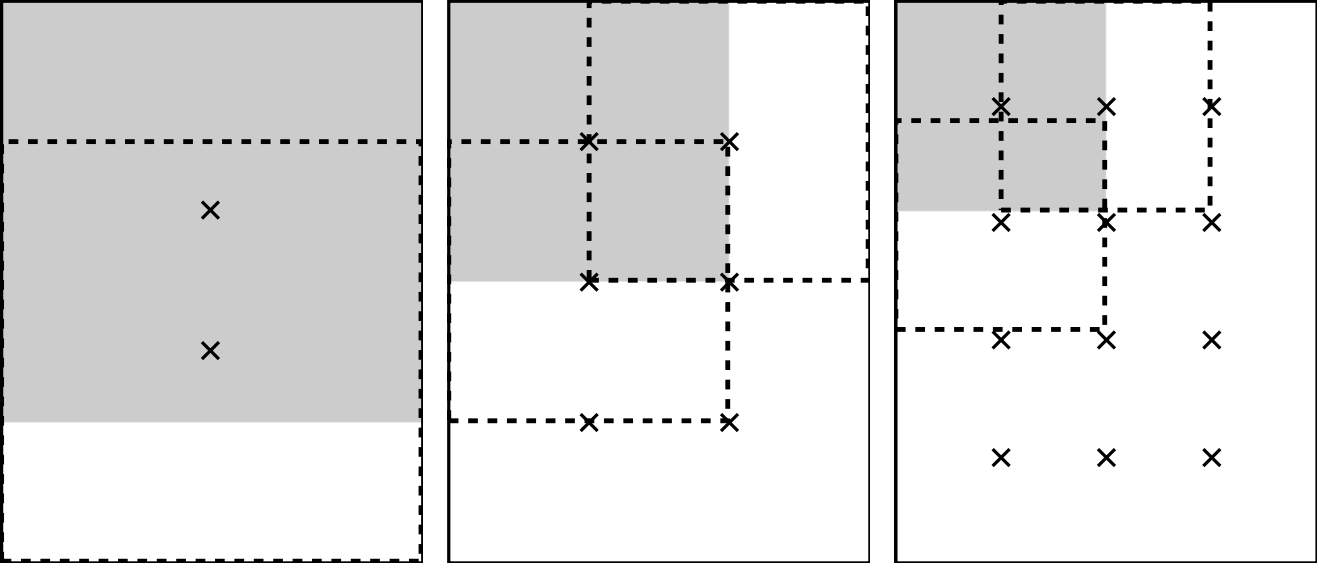
\includegraphics[width=0.6\linewidth]{img/rmac-regions}
    \caption{Example of regions chosen to extract the \gls{rmac} image descriptor from a \gls{cnn} feature map. \figfrom{tolias2016rmac}}
    \label{fig:back:rmac-regions}
\end{figure}

\paragraph{Learning Representations for Retrieval}
Representations obtained by transfer learning and their aggregation demonstrated the potential of features extracted by \glspl{cnn}.
Succeeding work further improved the state of the art by learning directly for the task of instance image retrieval.
% Babenko et al (2014): classif loss
% (Gordo et al, 2016): pretrained models finetuned for retrieval?
% (Radenovic et al, 2016): pretrained models finetuned for retrieval?
% \cite{arandjelovic2016netvlad}: NetVLAD

% FROM Gordo: A preliminary version of our work (Gordo et al, 2016), together with a concurrent work (Radenovic et al, 2016), confirmed that finetuning the pretrained models for retrieval can bring a significant improvement, but demonstrated that even more crucial are the combination of i) a good image representation and ii) a ranking loss – as opposed to the classification loss used by Babenko et al (2014).
% From Gordo RMAC+: Here, we argue that one of the main reasons that prevented previous retrieval methods based on deep architectures to perform well is their lack of supervised learning for the specific task of instance-level image retrieval~\cite{radenovic2016cnn,gordo2017end}. In this work, we focus on the problem of learning representations that are well suited for the retrieval task.
%The recent NetVLAD~\cite{arandjelovic2016netvlad} also highlights the importance of learning to rank.

% RMAC+
\subsection{Cross-modal Image Retrieval}
%Cross-modal Retrieval
%Textual / visual / common space retrievals


\subsection{Evaluation Metrics}
The image retrieval problem is not so different from classical textual information retrieval problem, thus it borrows from it much of the terminology, formulations and evaluation metrics.
% accuracy, computational cost, memory consumption
The main aspects to be considered in the evaluation of a retrieval system are its accuracy and its computational \& memory consumption in both the off-line and on-line stages.
While measuring computational and memory resources in this scenario is straightforward, researches dedicated multiple metrics to measure the accuracy of a retrieval system.
In the following paragraphs, we will introduce the notation and some of the conventionally used evaluation metrics.

Given a collection of images $\X$ and a query image $\q$, the goal is to retrieve the set of images $\X_q \subset \X$ relevant to $\q$.
In the feature-based approach, an image is represented by its feature vector $\x$, and a similarity $s(\cdot)$ (or distance $d(\cdot)$) function is defined to compare two feature vectors.
This function permits to assign a similarity score (or a distance) to each element of our search collection and to sort them based on their relevancy to the query.
Since the top elements on the candidate list are the ones to be most plausible to be consumed by the user, many of the evaluation metrics for measuring the accuracy of a retrieval system are thought to evaluate the goodness of the initial part of the results list.

Assume $\X$ %$= {\x_1, \ldots, \x_N}$
is a collection of $N$ elements, $\q$ a query, $\Y^{\star}_{\q} \subset \X$ the subset of $\X$ relevant to $\q$, and $\Y_{\q}$ the retrieved candidate set to be evaluated.
% = {\y_1, \ldots, \y_N} \subset \{0,1\}^N$ a set of $N$ indicator variables where $\y_i = 1$ if $\x_i$ is relevant for $\q$, 0 otherwise.
% PR
\paragraph{Precision and Recall}
With \emph{precision}, we refer to the fraction of retrieved samples that are relevant to the query
\begin{equation} \label{eq:back:precision}
\mathrm{Precision} = \frac{|\Y_{\q} \cap \Y^{\star}_{\q}|}{|\Y_{\q}|} \,,
\end{equation}
where $|\cdot|$ indicates the cardinality of a set.
We refer to the fraction of relevant samples actually retrieved as \emph{recall}
\begin{equation} \label{eq:back:recall}
\mathrm{Recall} = \frac{|\Y_{\q} \cap \Y^{\star}_{\q}|}{|\Y^{\star}_{\q}|} \,.
\end{equation}

A trade-off between precision and recall is often tuned on deployment;
the system may be tuned to retrieve only objects similar to the query with high confidence thus achieving high precision, but may leave behind some relevant samples and obtaining a low recall.
Viceversa, a less stringent retrieval has a high recall, but more retrieved samples may not be relevant to the query, decreasing the precision of the system.

% mAP
\paragraph{\acrlong{ap}}
The \emph{\acrfull{ap}} metric is commonly used to evaluate a retrieval system independently from the particular configuration of precision-recall.
Similarly to the \acrfull{auc} of ROC plots -- discussed in \ref{subsec:back:classif-eval} -- the \gls{ap} represent the area under the precision-recall curve and is computed as
\begin{equation} \label{eq:back:ap}
    \mathrm{AP} = \sum_r p(r)\,,
\end{equation}
where $r$ is the set of possible recall values that can be achieved, e.g. varying the maximum number of elements to be retrieved or the threshold on the scores of the retrieved samples.
When multiple queries are considered for evaluation, the \emph{\acrfull{map}} is usually reported, which is the mean of the \glspl{ap} obtained from each query.

%nDCG
\paragraph{\acrlong{dcg}}
The \emph{\acrfull{dcg}}~\cite{jarvelin2002cumulated} is conventionally used when multiple level of relevancy are available for samples in the groundtruth.
Its aim is to penalize highly relevant samples in the bottom part of the results;
to do so, usually a logarithmic weighting scheme is adopted to assign a decreasing importance to samples in the lower part of the search results.
The \gls{dcg} at the rank position $n$ is defined as
\begin{equation} \label{eq:back:dcg}
    \mathrm{DCG}@n = \sum_{i=1}^n \frac{2^{r_i} - 1}{\log_2(i + 1)} \,,
\end{equation}
where $r_i$ is a positive scalar representing the relevance of the $i$-th retrieved sample.
In the case rankings can have ties, the \gls{tdcg}~\cite{mcsherry2008computing} is used, defined as:
%
\begin{equation}
\mathrm{TDCG}@n = \sum_{i=1}^{m}\left(\left(\frac{1}{n_i}\sum_{j=t_i+1}^{t_{i+1}}2^{rel_i}-1\right)\sum_{j=t_i+1}^{\min(t_{i+1},k)}\frac{1}{\log_2(i+1)}\right)
\end{equation}
%
where $m$ is the number of group of ties in the ranking of the first $n$ results, $n_i$ indicates the number of tied result in the $i$-th group, $t_i$ indicates the starting position of each tied group.
The $TDCG$ is derived from $DCG$ by observing that the average gain for a position in a group of tied results is the average of the gain of such tied results.
The $TDCG$ is obviously equivalent to $DCG$ in the case there are no ties in the results.

% NDCG is divided by a normalization factor to ensure the metric is in the $[0,1]$ range.

% R@K
\paragraph{\acrlong{r@k}}
The \acrfull{r@k} is the recall metric when considering only the top-K results of the groundtruth as relevant.
It is conventionally used to compare two rankings in absence of an explicit relevancy labelling of the groundtruth.
Assuming $\Y^{\star}_{\q, K}$ the set of samples relevant to $\q$ truncated at the $K$-th element, and $\Y_{\q,K}$ the top-$K$ retrieved elements to be evaluated, the \gls{r@k} is defined as
\begin{equation} \label{eq:back:r@k}
    R@K = \frac{|\Y^{\star}_{\q, K} \cap \Y_{\q,K}|}{K} \,.
\end{equation}

%medR
\paragraph{\acrlong{medR} and \acrlong{mrr}}
These metrics are particularly useful when evaluating rankings in which there is only one object in the database relevant to the query that need to be retrieved.
Cross-modal retrieval with coupled datasets is an examples in which this condition applies: using as query one modality of a sample, a common approach is to evaluate how well the system is able to retrieve the same sample in the different modality.
Given multiple queries, the \acrfull{medR} is the median of the positions of the relevant objects in the rankings, one per query,
% MRR
while the \acrfull{mrr} is the mean of the reciprocals of the same quantities.


\subsection{Image Indexing}
%\label{sec:back:indexing}
%kNN schemes
%Permutation-based representations
%Deep Permutations

%Datasets & Evaluation Metrics

\section{Datasets}
\label{sec:back:datasets}
In this section, we will list the dataset -- either publicly available or collected -- used directly or indirectly in the experiments presented in this work.

\subsection{Classification Datasets}

\paragraph{\acrfull{ilsvrc} 2012~~\cite{russakovsky2015imagenet}}
The \acrfull{ilsvrc} 2012 dataset is composed by a large set of images of general objects collected for evaluating algorithms for large-scale visual object recognition.
It is a subset of roughly 1.3 million images taken from the larger ImageNet\footnote{\url{http://www.image-net.org}} database -- a big collection of images labelled and organized following the hierarchical categorization of WordNet.
Images are assigned a single label chosen from the 1,000 classes selected for the competition, spanning general objects, animals, etc.
Each class has roughly 1,000 images in the training set (the number oscillates between 700 and 1,300), and exactly 50 and 100 images respectively in the validation and test set, for a total of 1,281,167 images for the train set, 50,000 for the validation set, and 100,000 in the test set.
Only the training and validation sets are publicly available.

\paragraph{Places205~\cite{zhou2014learning}}
The Places205 dataset is composed by roughly 2.5 million images collected from image search engines labelled with 205 semantic scene categories and attributes representing visual environments all over the world.
It is a subset of the bigger Places dataset~\cite{zhou2016places}.

\paragraph{PKLot~\cite{de2015pklot}}
The PKLot dataset is an car parking occupancy detection dataset comprised by 12,417 images of 3 parking lots, named UFPR04, UFPR05, and PUC, took in different days and weather conditions.
The images have been segmented in 695,899 images of parking spaces by cropping along the rotated rectangles delimiting each parking space and rotating back the cropped patches in vertical or horizontal position.
Each segmented image is labelled with the vacancy status of the slot, which can be either occupied or vacant.

\paragraph{CNRPark+EXT~\cite{amato2016car,amato2017deep}}
The CNRPark+EXT dataset is a car parking occupancy detection dataset collected during this thesis from the parking lots of the campus of the National Research Council (CNR) in Pisa.
It is comprised by roughly 150,000 images of parking spaces taken from 9 smart cameras with different view-points, in different days with different weather and light conditions, and includes occlusion and shadow situations that make the occupancy detection task challenging.
More details about the CNRPark-EXT dataset will
be given in \ref{ch:deep-parking}.

\paragraph{Twitter Testing Dataset~\cite{you2015robust}}
The Twitter Testing Dataset is a dataset for image sentiment analysis composed by 1269 images labelled with crowd-sourcing (Amazon Mechanical Turk) following a binary positive/negative sentiment polarity scheme.
Each image has been annotated as positive or negative by five workers, and three different subsets have been created, respectively comprised by images where 5 workers agree on the sentiment of the image (5-agree, 882 images), where at least 4 workers agree (4-agree, 1,116 images), and where at least 3 workers agree (3-agree, whole set of images).

\paragraph{\acrfull{t4sa}~\cite{vadicamo2017cross}}
The \acrlong{t4sa} dataset is a large-scale weakly-labelled dataset for sentiment analysis collected during this thesis to evaluate the weakly-labelled cross-media training procedure for image classifiers presented in \ref{ch:weakly-labelled}.
It is comprised by 904,395 tweets and their corresponding 1,473,394 images (each tweet has one or more images);
tweets have been collected from the 5\% random stream of global tweets provided by the Twitter APIs keeping only tweets in english with at least five words and at least one image.
Each tweet is associated with a three-way sentiment polarity (positive/neutral/negative sentiment) predicted by performing textual sentiment polarity prediction.
More details are available in \ref{ch:weakly-labelled}.

\subsection{Retrieval Datasets}

\paragraph{INRIA Holidays~\cite{jegou2008hamming}}

The INRIA Holidays image set is an image retrieval dataset comprised by 1491 high-resolution holidays photos containing various scenes types.
The authors chose 500 queries and manually selected from the set the images relevant for each query.
A frequently used variant of this dataset is the one augmented with \emph{MIRFlickr1M}, a distractor set of 1 million images collected by the Flickr service;
we refer to this new dataset as \emph{Holidays-MIRFlickr1M}.

\paragraph{Oxford Buildings~\cite{philbin2007object}}
The Oxford Buildings dataset, also known as \emph{Oxford5k}, is an image retrieval dataset comprised by 5,062 images of various buildings present in Oxford.
The set is composed by photos of 11 famous buildings plus distractor images collected from Flickr.
For each building, five queries are specified with bounding boxes delimiting the building we are interested in retrieving, for a total of 55 query images.
For each query, images of the search set are assegned with one of the following four labels:
\begin{itemize}
    \item \emph{ok} -- if the image contains a clear look of the building in the query;
    \item \emph{good} -- if more than 25\% of the building is clearly visible;
    \item \emph{junk} -- if less than 25\% of the building
is visible, or there is a very high level of occlusion or dis-
tortion;
    \item \emph{absent} -- if the building is not present.
\end{itemize}
In this work, we will adopt the version of this dataset augmented with a distractor set of 100k images collected from Flickr, and we will refer to it as \emph{Oxford-Flickr100k}.

% \paragraph{Paris~\cite{philbin2008lost}}
% \paragraph{Flickr100k and Flickr1M ~\cite{philbin2007object}}

\paragraph{\acrfull{coco}~\cite{lin2014microsoft}}

The Microsoft \acrfull{coco} dataset is a collection of images  for large-scale object detection, segmentation, and captioning.
it is comprised by 2,500,000 labeled object instances belonging to 91 common object categories in 328,000 images.
Each image is associated with an instance-level pixel-wise segmentation of the object instances it depicts and five captions describing the whole images.
This dataset is particularly adopted also in cross-modal retrieval due to its large scale and the presence of captions, and we will use it to compare to existing cross-modal retrieval approaches in \ref{ch:text-to-vis}.

\subsection{Others}

\paragraph{NIPS Adversarial Attacks and Defences Competition DEV set~\cite{kurakin2018adversarial}}
The NIPS Adversarial Attacks and Defences Competition DEV set is comprised by 1,000 images that do not belong to the \gls{ilsvrc}'12 subsets but share the same label space, i.e. are labelled with one of the same 1,000 label used in \gls{ilsvrc}.
This set has been released in the context of the NIPS Adversarial Attacks and Defences Competition on Kaggle to let participants work with pre-trained \gls{ilsvrc} classifiers using images not involved in their training process.
In particular, the set is devoted to generate adversarial examples for image classifiers, i.e. maliciously manipulated images the lead a classifier to misbehave.
More details are available in \ref{ch:detect-advesarial} in which we use this set of images to evaluate a detection scheme for adversarial attacks.

%======================= MINIATURIZE CNN FOR EMBEDDING ===========================

%TODO uniforma view-point viewpoint
%TODO uniforma \emph{AlexNet} e AlexNet
%TODO captions

\graphicspath{{img/parking/}}

\chapter{Miniaturization of Convolutional Neural Networks for Embedded Devices}
\label{ch:miniaturization}

One of the most important limitations of \glspl{dcnn} is that they often rely on computationally expensive deep models, which are slow for many applications including image classification.
Due to this limitation, methods based on efficient hand-crafted local features --- such as \acrshort{surf}, \acrshort{orb}, \acrshort{lbp}, etc.\ --- are predominantly adopted in vision systems where a computational power of a full-featured server is not available, e.g.\ mobile phones or embedded devices.

In this chapter, we will explore the adoption and the miniaturization of \glspl{dcnn} for efficient image classification.
We focus our investigation on reducing and evaluating deep models for embedded vision systems, i.e.\ smart cameras.
A smart camera is an embedded camera equipped with a limited computational and communication capabilities that can be used to process, extract, and send information contained in the captured images on board of the device itself.
% TODO [CITE] smart surveillance or campus with CNNs
Empowering smart cameras with the generalization and robustness of \glspl{cnn} for computer vision application represents one the most promising steps towards the evolution of smart environments \cite{}.
Their ``smart'' nature makes them suitable for automated intelligent systems able to generate event descriptions and/or make decisions \cite{belbachir2010smart}, thus making them attractive to a broad range of applications.
In our study, we will focus on a specific application, that is the visual occupancy detection of outdoor car parking lots in a decentralized fashion with smart cameras.
The motivation for the choice of this specific problem is manyfold.
\begin{itemize}
	% easy problem formulation as 2-way classification
	% lack of deep learning solutions for the problem
	\item The problem of visual occupancy detection of parking spaces can be easily formulated as a binary image classification problem;
	this enable us to focus on the engineering aspects about model reduction and its evaluation;
	moreover state-of-the-art approaches tackling this problem are based on hand-craft features and shallow machine learning, while a deep learning solution could (and will) bring an improvement of the detection accuracy and robustness.

	% current systems vision solutions are centralized, with BW costs
	\item Parking lot occupancy detection systems are commonly implemented by means of expensive magnetic ground sensors, while vision-based systems provide a more cost-effective solution;
	in our setup, a single smart camera can simultaneously monitor up to 50 parking slots at a cost significantly lower than the one required to install and maintain ground sensors for every slot.

	% decentralize for flexibility and bw cost
	\item In centralized solutions, ``dumb'' cameras send their video feeds to a server which process them;
	a decentralized solution instead brings a reduction of the communication overhead and the elimination of the computing bottleneck, thus increasing even further the scalability of the solution;
	moreover, an intelligent infrastructure provides flexibility in its application, e.g.\ the same cameras could be used for perimeter surveillance during night hours.

\end{itemize}

While visual approaches to parking lot occupancy detection are not new \cite{dan2002parking,wu2007robust,del2015vacant,de2015pklot}, the usage of solely visual information still poses challenges in terms of robustness.
Numerous solutions are tailored to specific scenarios and hardly generalize well to different ones, such as a different parking lot, view-point, light conditions, or occlusion patterns.

In our investigation, we propose a decentralized and efficient vision system based on smart cameras and \gls{dl} for parking lot occupancy detection.
We present a reduced \gls{dcnn} suitable for embedded devices with which we implement the classification logic under the occupancy detection task.
A strong experimental protocol on publicly available datasets is applied to compare the proposed approach to the state-of-the-art methods and deep models and assess the its generalization properties.
In addition, we contribute with a publicly available dataset of the parking lot images captured by multiple cameras called \emph{CNRPark-EXT} that enables us to thoroughly test the robustness of our solution to multiple source of errors.

The chapter is organized as follows.
In \ref{sec:mini:related-work}, we introduce the work related to parking lot occupancy detection, focusing on vision-based solutions more related to our proposal.
In \ref{sec:mini:occupancy-detection}, we propose and describe the \gls{dcnn} model specifically designed to be executed on smart cameras which implements the parking slot classification pipeline.
In \ref{sec:mini:datasets}, we presents the already available and newly collected datasets used to evaluate and compare our approach.
\ref{sec:mini:evaluation} presents the proposed experimental setup to compare the our approach to the state of the art and evaluate its robustenss to multiple aspects.
\ref{sec:mini:deployment} briefly describes the deployment of our solution in a real scenario and gives an overview of the overall system.

The research presented in this chapter was published in~\cite{amato2016car,amato2017deep}, and the provided resources --- e.g.\ datasets and trained models --- are available at \url{http://cnrpark.it}.

\section{Visual Occupancy Detection and Related Work}
\label{sec:mini:related-work}

Techniques for car parking occupancy detection are of great importance for an effective management of car parking lots.
Knowing in real-time the availability of free parking spaces and communicating it to the users can be of great help in reducing the queues, traffic jams, and the time required to find an available parking slot.
In the following paragraphs, we will review some of the work targeting this problem, focusing on vision-based methods.

\paragraph{\gls{ml}-based approaches}
% Occupancy Detection w/o CNNs
Many attempts before the \gls{dl} era were implemented by classical \gls{ml} methods applied on hand-crafted visual features.
\citet{dan2002parking}, one of earliest work using this approach on the subject, used \glspl{svm} on color features to classify regions of the parking lot as `car` or `empty-space`.
Among the challenges arose by the task, the problem of occlusions due to obstacles or camera angle is one of the most significant.
\citet{wu2007robust} tried to overcome occlusion by neighboring cars by considering also the neighbor parking slots of the one to be classified.
The \gls{svm} classifier for a slot is defined over the colour features computed across three slots (the slot itself and the two neighbor slots).
\citet{tsai2007vehicle} used multiple hand-crafted features and a Bayesian classifier to deal with the problem of light changes, while
\citet{huang2013vacant} employed a Bayesian hierarchical framework based on a 3D model of the parking spaces.
Similarly, \citet{delibaltov2013parking} proposed a method based on a 3D model of every parking slot in order to account for occlusions when classifying a slot as vacant or occupied.
In~\cite{jermsurawong2014one}, a customized neural networks based on visual features is used to model the occupancy status of slots and the parking demand. % TODO check paper
% they present robust results for night and day classifiers in a one-day long evaluation based on 126 parking spaces.
In~\cite{de2015pklot}, the authors employed ensembles of \gls{svm} classifiers based on multiple textural features --- such as \gls{lbp}, \gls{lpq}, and their variations --- and they present a dataset of roughly 700,000 images of parking spaces coming from three different cameras used in their experiment.
\citet{del2015vacant} proposed a temporal analysis of the video frames based on background subtraction to detect and track parking and leaving vehicles.
In a similar fashion, \citet{masmoudi2014} propose to overcome the occlusion problem by visually tracking cars entering or leaving a parking space.

\paragraph{Non-vision approaches}
In addition to approaches using visual techniques and commercial solutions using ground sensors, there are techniques harnessing sensors installed on cars or carried by the drivers.
In \cite{caicedo2012prediction}, the authors argue that occupancy detection can be solved by interacting with smart in-vehicle navigation systems.
\citet{lan2014intelligent} instead proposed to harness sensors in smart phones and other devices to collect real-time parking availability information.
%
\paragraph{\gls{dl}-based approaches}
To the best of our knowledge, the proposed approach is the first work that employs \glspl{dcnn} in the context of parking lot monitoring.
A relevant work in a similar --- yet different --- task is \cite{chen2014vehicle}, where the authors employed a multi-scale \gls{cnn} to detect vehicles in high-resolution satellite images.

\section{\glspl{dcnn} for Occupancy Detection in Embedded Devices}
\label{sec:mini:occupancy-detection}

\begin{figure}
	% TODO [FIGURE] alex e malex a confronto
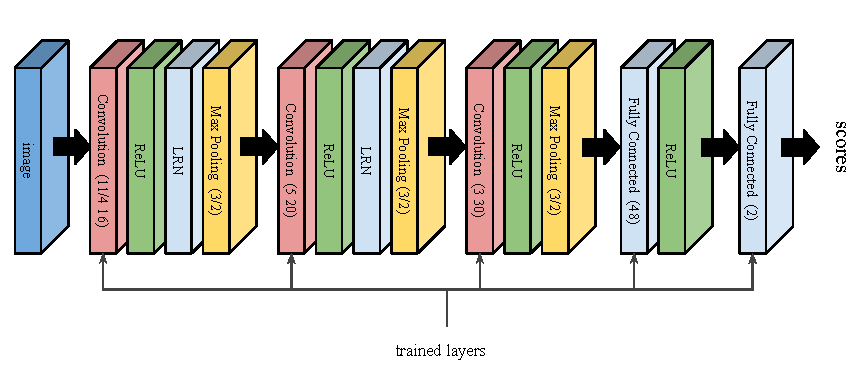
\includegraphics[width=\linewidth]{net-archit}
% 	\newcolumntype{Y}{>{\centering\arraybackslash}X}
% 	\begin{tabularx}{\textwidth}{|Y|Y|Y|Y|Y|Y|}
% 		% \begin{tabular}{|c|c|c|c|c|c|}
% 		\hline
% 		\emph{net} & \emph{conv1} & \emph{conv2} & \emph{conv3} & \emph{fc4} & \emph{fc5} \\ \hline \hline
% %		             & 30x11x11+4     & 20x5x5+1       &                & 100          & 2            \\
% %		mLeNet       & pool 5x5+5     & pool 2x2+2     & -              & ReLU         & soft-max     \\
% %		             & -              & -              &                &              &              \\ \hline \hline
% 		             & 16x11x11+4     & 20x5x5+1       & 30x3x3+1       & 48           & 2            \\
% 		mAlexNet     & pool 3x3+2     & pool 3x3+2     & pool 3x3+2     & ReLU         & soft-max     \\
% 		             & LRN, ReLU      & LRN, ReLU      & ReLU           &              &              \\ \hline
% 	\end{tabularx}
\caption{CNN Architecture: for convolutional layers \emph{conv1-3}, parameters are specified as ``$size/stride~num$''.
For max-pooling, parameters are specified as ``$size/stride$''.
For fully connected layers we report their dimensionality.
The last fully connected layer is followed by a 2-way softmax classifier.}
\label{fig:mini:cnns}
\end{figure}

% \begin{table}

% 	\caption{CNN Architecture: for convolutional layers \emph{conv1-3} the
% 		first row in a cell specifies the number and the size of filters as
% 		``$num \times width \times height + stride$''. The second row specifies
% 		the max-pooling operation applied as ``$width \times height + stride$''.
% 		The third row indicates if Local Response Normalization (LNR) and/or
% 		Rectified Linear Unit (ReLU) activation are applied. For fully connected
% 		layers we report their dimensionality. The last fully connected layer
% 	    is followed by a 2-way soft-max classifier.}
% 	\label{tbl:cnns}
% \end{table}

\noindent The main objective of our proposal is to design a \gls{cnn}-based classifier for the problem of occupancy detection runnable by smart cameras and low-power embedded devices in general.
Due to its popularity and wide-spread adoption, we adopted the Raspberry Pi 2 model B \footnote{\url{https://www.raspberrypi.org/products/raspberry-pi-2-model-b/}} equipped with the standard Raspberry Pi camera module \footnote{{https://www.raspberrypi.org/documentation/hardware/camera.md}} as a reference hardware implementation of a smart camera.

As done in previous work, we formulate the visual occupancy detection of a parking slot as a binary classification problem in which an image of a single parking space is either labelled as \emph{vacant} or \emph{occupied}.
We assume that the cameras are fixed, and each of them monitors several parking slots.
The images of the individual slots are obtained from the entire frame by cropping fixed regions that have been manually defined off-line, and the smart camera is in charge of performing an independent classification for each image.

% TODO [CITE] AlexNet applications
As a starting point for the design of our solution, we considered the very popular \emph{AlexNet} \gls{cnn} for image classification~\cite{krizhevsky2012imagenet}, which is used as reference in many computer vision applications~\cite{}.
Such architecture exploits its massive number of parameters to learn a non-linear mapping from pixels to high-level features that facilitate classification.
However, its computational budget and memory footprint poses severe limitations on devices with limited resources,
especially when taking into account that the number of monitored slots per camera can easily reach 50--100.
Moreover, considering that a forward pass of AlexNet on the Raspberry Pi model B on a 224x224 RGB image takes roughly 20 second while occupying most of the RAM available on the device\footnote{Data collected using the implementation of AlexNet of the Caffe~\cite{jia2014caffe} library}, it is evident that this architecture does not scale to the size of the problem.

We argue that the problem of visual occupancy detection --- despite the presence of high variability factors such as changing light conditions, viewpoints, and occlusion patterns --- is less complex with respect to the \gls{ilsvrc}'12 classification task AlexNet was designed for.
We define a reduced \gls{dcnn} architecture --- named \emph{miniAlexNet} or simply \emph{mAlexNet} --- to implement a simplified classifier, and we compare its performance and computational cost with respect to the original AlexNet.
The architecture of \emph{mAlexNet} follows the AlexNet one.
We keep the dimensionality of the input unaltered, i.e.\ a $224 \times 224$ RGB image, that in our scenario will contain the visual appearence of a single parking slot.
In case of differently-sized images, they are resized to match the input dimensionality.
We reduced the number of convolutional layers from five to three, the first two followed by max-pooling, \gls{lrn}, and \gls{relu} activations, while in the third one, the \gls{lrn} is omitted.
The number of fully-connected layers is reduced to two, including the one producing the final prediction.
We drastically reduced the number of filters and neurons of all layers, starting from the minimalist number of 16 filters in the first convolution layer and defining the dimensionality of subsequent layers following the proportions of the original architecture.
We argue that a small number of convolutional filters in the first layer are sufficient to detect low-level features important for the task --- such as edges and corners with multiple rotations --- while reducing the possibility of overfitting.
We maintained the convolutional kernel sized and pooling sizes of the original architecture, since we share the same image input shape.
The obtained model has roughly 42,000 parameters, that is roughly $1360 \times$ less with respect to AlexNet.
\ref{fig:mini:cnns} reports the details of the proposed architecture.
As confirmed by experiments reported in \ref{sec:mini:evaluation}, using a smaller model for visual occupancy detection does not entail a severe performance degradation.
The Caffe implementation of our model is able to perform on average 50 parking slot classifications on a single Raspberry Pi model B in roughly 15 seconds, which is an acceptable cycle time for parking lot occupancy detection systems. % TODO? note on new impl?
The training phase, which need a considerable amount of computational resources, is performed off-line once on a powerful device, and the final classification model is deployed on multiple smart cameras once it is trained.

\section{Datasets}
\label{sec:mini:datasets}

In this section, we will describe the two datasets used to train and evaluate our proposed parking slot classifier.

\paragraph{PKLot}
The first dataset, PKLot~\cite{de2015pklot}, includes 695,899 images of parking slot extracted from photos of two parking lots --- dubbed UFPR and PUC --- taken by three cameras in multiple weather conditions and spanning different days.
Two cameras captured images of the UFPR parking lot from two different view-points identified by the names UFPR04 and UFPR05, while the other one is dedicated to the PUC lot.
Slot images are obtained from the full camera frame by manual segmentation of non-occluded and non-overlapping spaces: rotated rectangles are placed on the image to precisely identify the slots in each parking lot, and regions are subsequently extracted from frames using the defined mask.
This segmentation strategy results in a precise coverage of the parking slot without strong forms of occlusion.
Extracted patches are then straightened to the nearest vertical or horizontal orientation depending on the orientation of the rotated rectangle used as mask.
Every patch is manually labelled either as `vacant` or `occupied`.

\begin{figure}
\centering
\begin{subfigure}[b]{0.49\columnwidth}
	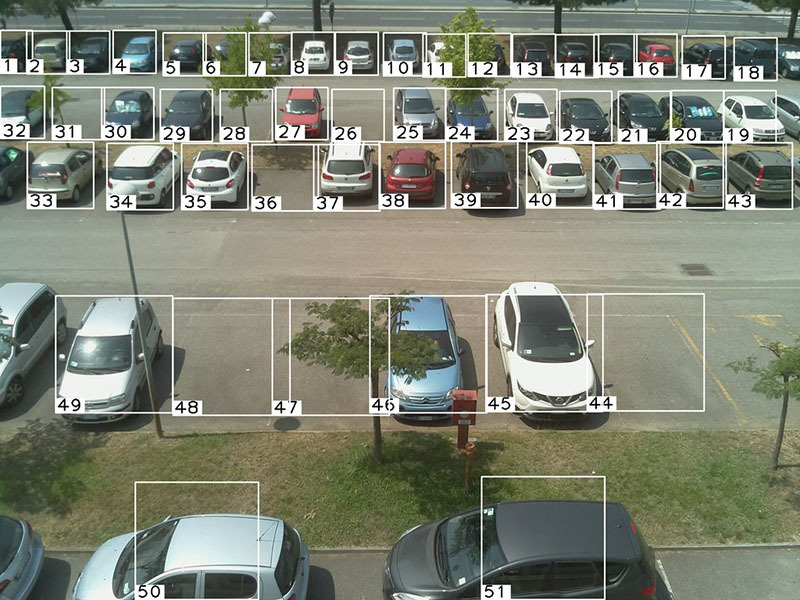
\includegraphics[width=\columnwidth]{camera-a-overview}
	\caption{Overview of CNRPark CAM A}
	\label{fig:mini:cam-a}
\end{subfigure} %
\begin{subfigure}[b]{0.49\columnwidth}
	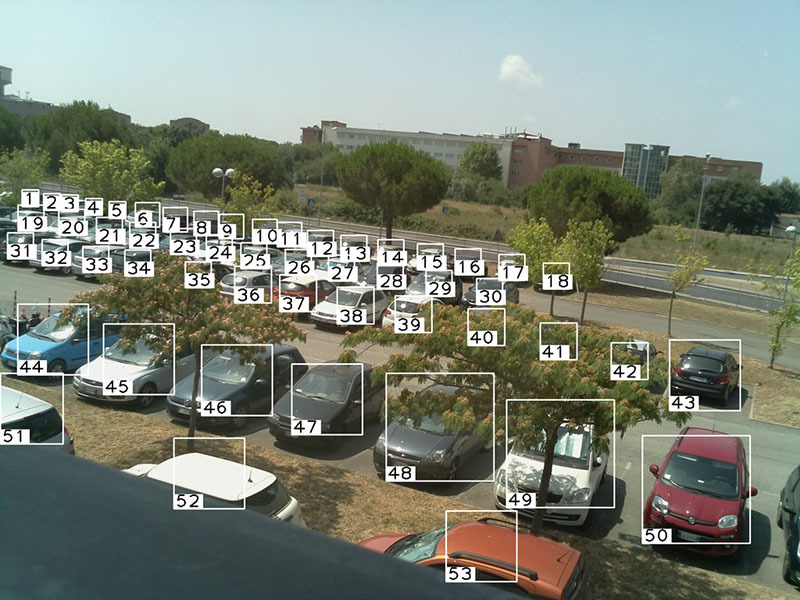
\includegraphics[width=\columnwidth]{camera-b-overview}
	\caption{Overview of CNRPark CAM B}
	\label{fig:mini:cam-b}
\end{subfigure}

\begin{subfigure}[b]{0.49\columnwidth}
	\includegraphics[width=\columnwidth]{overview-cam1}
	\caption{Overview of CNRPark-EXT CAM 1}
	\label{fig:mini:cam-1}
\end{subfigure} %
\begin{subfigure}[b]{0.49\columnwidth}
	\includegraphics[width=\columnwidth]{overview-cam8}
	\caption{Overview of CNRPark-EXT CAM 8}
	\label{fig:mini:cam-8}
\end{subfigure}
\caption{Segmentation masks for parking slot images in the preliminary \emph{CNRPark} dataset (top) and in the extended \emph{CNRPark-EXT} dataset (bottom, only for camera 1 and 8)}
\label{fig:mini:cam-overview}
\end{figure}

\begin{figure}
\begin{subfigure}{0.25\columnwidth}%
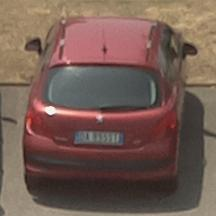
\includegraphics[width=\columnwidth]{38busy}%
\end{subfigure}%
\begin{subfigure}{0.25\columnwidth}%
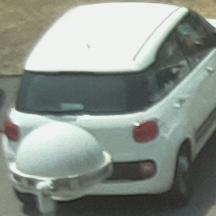
\includegraphics[width=\columnwidth]{34busy}%
\end{subfigure}%
\begin{subfigure}{0.25\columnwidth}%
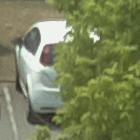
\includegraphics[width=\columnwidth]{11busy}%
\end{subfigure}%
\begin{subfigure}{0.25\columnwidth}%
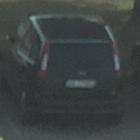
\includegraphics[width=\columnwidth]{13busy}%
\end{subfigure}

\begin{subfigure}{0.25\columnwidth}

\includegraphics[width=\columnwidth]{38empty}%
\end{subfigure}%
\begin{subfigure}{0.25\columnwidth}%
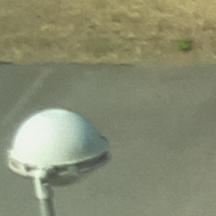
\includegraphics[width=\columnwidth]{34empty}%
\end{subfigure}%
\begin{subfigure}{0.25\columnwidth}%
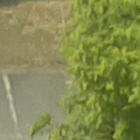
\includegraphics[width=\columnwidth]{11empty}%
\end{subfigure}%
\begin{subfigure}{0.25\columnwidth}%

\includegraphics[width=\columnwidth]{13empty}%
\end{subfigure}
\caption{Example of segmented parking slots images under different light conditions and occlusion patterns.
The first and second rows show four slots respectively in `occupied` and `vacant` state}
\label{fig:mini:slots}
\end{figure}

\paragraph{CNRPark}
In order to measure the generalization power of the proposed approach to unseen scenarios, we personally built a new dataset --- named \emph{CNRPark} --- collecting images from the parking lot in the campus of the National Research Council (CNR) in Pisa.
The preliminary version of this dataset --- which we refer to as CNRPark --- contains roughly $12,000$ images of slots of a part of the parking lot which were collected from 2 Rasperry Pi cameras (denoted as camera $A$ and $B$) with different perspectives and angles of view in different days of July 2015 (see \ref{fig:mini:cam-a,fig:mini:cam-b}).
Images of individual parking slots are extracted using manually-placed squared masks from the full camera frame.
Slot masks are placed to minimize the part of adjacent slots contained in the image, often limiting the area usable for classification to just a part of the entire slot.
Moreover, in many slots, occlusions by adjacent cars and obstacles (e.g.\ trees, lampposts) are inevitable due to the skewed field of view of the cameras;
this also involves that slots images have different sizes depending on the distance of the slot from the capturing camera.
Thus, our dataset poses additional challenges to occupancy detection methods that can be commonly found in real scenarios.
We split the dataset in two non-overlapping sets named \emph{CNRParkOdd} and \emph{CNRParkEven} respectively containing slot images having odd or even slot id.
This permitted us to test the generalization of our approach by training on some slots and test on unseen slots.

\paragraph{CNRPark-EXT}
We subsequently extended the CNRPark dataset gathering more images of the complete parking lot --- comprised by 164 parking slots --- captured by 9 additional cameras from November 2015 to February 2016.
\ref{fig:mini:cam-1,fig:mini:cam-8} report the cameras with respectively the most and least skewed views.
Images were collected in multiple days spanning multiple seasons of the year, and the number of slots monitored by each camera roughly spans from 10 to 50.
To extract the images of individual slots, we followed the same strategy of CNRPark.
The extended version of the dataset --- dubbed \emph{CNRPark-EXT} -- is composed of 4,287 camera frames acquired in 23 different days, from which we obtained 144,965 manually labeled images of individual parking slots.
The added value of our dataset stands in the fact that it captures a variety of occlusion and shadow patterns, and light and weather conditions (see \ref{fig:mini:slots}) that cover more real-case scenarios with respect to existing datasets.
Slot images are grouped by camera ID, by time of capture, and by three weather conditions --- i.e.\ \emph{Sunny}, \emph{Overcast}, and \emph{Rainy}.
We also provide splits for training, validation, and test sets;
we ensured that images captured in a particular day do not span more than one set.

\ref{tab:mini:datasets} reports detailed information about the composition of \emph{CNRPark}, \emph{CNRPark-EXT}, and \emph{PKLot}~\cite{de2015pklot}.
The main difference between our datasets and the existing ones can be summarized as follows.
Slot images in \emph{CNRPark-EXT} often do not cover precisely or entirely the parking slot volume, whereas in \emph{PKLot} slots are registered and straightened, resulting in a more precise coverage of the parking slot.
Moreover, \emph{CNRPark-EXT} captures heavily occlusion patterns (some slots are almost entirely covered by trees and lampposts) and lower point of views, resulting in considerable occlusions due to adjacent vehicles.
Even if our dataset counts less images than \emph{PKLot} and has been collected from a single parking lot, we assessed through experiments that the real challenge comes from the variety of view-points and occlusions patterns of which our dataset is rich:
in fact, we let the \gls{cnn} to cope with these factors, resulting in a more robust classifiers in real case scenarios and in a reduced manual setup effort.

\begin{table}
\newcolumntype{R}{>{\raggedleft\arraybackslash}X}
% \def\arraystretch{1}
\begin{tabularx}{\linewidth}{lRRR}
\toprule
\textsc{Dataset}    & \textsc{vacant} & \textsc{occupied} & \textsc{total} \\
\midrule
%                       &               &               &                \\
%    CNRPark $A$       & 2549          & 3622          & 6171           \\
%    CNRPark $B$       & 1632          & 4781          & 6413           \\ \hline
%    CNRPark           & 4181          & 8403          & 12584          \\

     CNRPark           & 4,181          & 8,403          & 12,584          \\
     CNRPark-EXT       & 65,658         & 79,307         & 144,965         \\
     PKLot             & 337,780        & 358,119        & 695,899         \\ %\hline
%                       &               &               &                \\
%    CNRPark TRAIN     & 2201          & 3970          & 10000          \\
%    CNRPark VAL       & 1980          & 4433          & 2584           \\ \hline
%    CNRPark           & 4181          & 8403          & 12584          \\
\bottomrule
                       &               &               &                \\
\toprule
\textsc{Subset} & \textsc{vacant} & \textsc{occupied} & \textsc{total} \\ \midrule
    CNRParkOdd        & 2,201          & 3,970          & 6,171           \\
    CNRParkEven       & 1,980          & 4,433          & 6,413           \\ %hline
\midrule
     CNRPark-EXT TRAIN     & 46,877         & 47,616         & 94,493          \\
     CNRPark-EXT VAL       & 5,232          & 13,415         & 18,647          \\
     CNRPark-EXT TEST      & 13,549         & 18,276         & 31,825          \\ %\hline
%     CNRPark-EXT           & 65658         & 79307         & 144965         \\
\midrule
     CNRPark-EXT SUNNY     & 25,665         & 37,513         & 63,178          \\
     CNRPark-EXT OVCST     & 21,067         & 23,176         & 44,243          \\
     CNRPark-EXT RAINY     & 18,926         & 18,618         & 37,544          \\ %\hline
%     CNRPark-EXT           & 65658         & 79307         & 144965         \\
\midrule
     CNRPark-EXT \emph{C1}      & 6,407          & 9,308          & 15,715          \\
     CNRPark-EXT \emph{C2}       & 1,454          & 2,641          & 4,095           \\
     CNRPark-EXT \emph{C3}       & 4,101          & 5,370          & 9,471           \\
     CNRPark-EXT \emph{C4}       & 7,219          & 9,357          & 16,576          \\
     CNRPark-EXT \emph{C5}       & 9,582          & 11,256         & 20,838          \\
     CNRPark-EXT \emph{C6}       & 9,462          & 10,646         & 20,108          \\
     CNRPark-EXT \emph{C7}       & 10,595         & 10,519         & 21,114          \\
     CNRPark-EXT \emph{C8}       & 11,237         & 12,847         & 24,084          \\
     CNRPark-EXT \emph{C9}       & 5,601          & 7,363          & 12,964          \\ %\hline
%     CNRPark-EXT           & 65658         & 79307         & 144965         \\
\midrule
%					   &               &               &                \\
     PKLot2Days        & 27,314         & 41,744         & 69,058          \\
     PKLotNot2Days     & 310,466        & 316,375        & 626,841         \\ %\hline
%     PKLot             & 337780        & 358119        & 695899         \\
%                       &               &               &                \\
\midrule
     PKLot UFPR04 TRAIN& 25,894         & 23,266         & 49,160          \\
     PKLot UFPR04 TEST & 33,824         & 22,859         & 56,683          \\
     PKLot UFPR05 TRAIN& 45,759         & 48,196         & 93,955          \\
     PKLot UFPR05 TEST & 22,600         & 49,230         & 71,830          \\
     PKLot PUC TRAIN   & 114,424        & 106,334        & 220,758         \\
     PKLot PUC TEST    & 115,616        & 87,895         & 203,511         \\ %\hline
%     PKLot             & 337780        & 358119        & 695899         \\
%                       &               &               &                \\
\midrule
     PKLot TRAIN       & 27,314         & 41,744         & 105,843         \\
     PKLot VAL         & 54,909         & 47,453         & 165,785         \\
     PKLot TEST        & 275,894        & 248,583        & 424,269         \\ %\hline
%     PKLot             & 337780        & 358119        & 695899         \\
\bottomrule
  \end{tabularx}
\caption{Details of datasets used in the experiments, with the various proposed subsets.
Values refer to the number of slot images contained in every dataset or subset}
\label{tab:mini:datasets}
\end{table}

\section{Evaluation}
\label{sec:mini:evaluation}

In this section, we present the experimental evaluation and discuss the obtained results.
Our investigation focused on getting insight on three main aspects of the proposed solution that can be summarized by the following questions:
\begin{enumerate}
\item How does our reduced classifier compare against state-of-the-art approaches?
\item How much the generalization performance degrades when using our reduced model instead of the original AlexNet architecture?
\item How much the proposed solution for visual occupancy detection is robust to weather and viewpoint changes?
\end{enumerate}

To answer these question, we extensively evaluated our approach using the two datasets described in \ref{sec:mini:datasets}, i.e.\ PKLot and CNRPark-EXT.
We performed experiments by splitting the datasets into several subsets that we will described in the following subsections.
Details about data splits are summarized in \ref{tab:mini:datasets}.
The usage of multiple methods on multiple datasets also permits us to compare the quality of our newly collected dataset for learning to detect occupancy detection robustly in real scenarios.

% -----

\subsection{Comparison with the State of the Art}
\label{sub:mini:sota}

We compared \emph{mAlexNet} against the state-of-the-art visual occupancy detection system proposed by \citet{de2015pklot}, which is based on \glspl{svm} classifiers with RBF kernels defined over hand-crafted textural features.
Specifically, histograms of \gls{lbp}, \gls{lpq} features and their variations \cite{ojala2002multiresolution, ojansivu2008blur, rahtu2012local} have been tested as input features of the \gls{svm}.
\Glspl{svm} are calibrated to output the probability of a slot to be occupied.
The authors also shown that the performance of the classification can be improved by using ensembles of \gls{svm} classifiers each defined on a particular textural feature:
probability values are fused using simple aggregation functions, such as \emph{Max} and \emph{Mean}, to obtain the final decision for an image slot.

We follow the experimental protocol described in \cite{de2015pklot}.
We split images from each camera of the PKLot dataset (UFPR04, UFPR05, and PUC) into a training and test set with roughly a 50\%--50\% proportion;
for a fair evaluation, we ensure that images collected in a particular day do not appear in both training and test set.
We then train both mAlexNet and the \glspl{svm} on each of the three training set, and tested on all the available test sets.
%
%Similarly, we also repeated the same protocol with our preliminary CNRPark dataset.
%We split CNRPark into two subsets --- CNRParkEven and CNRParkOdd --- respectively containing images of slots having even and odd IDs.
%We train both \glspl{svm} and mAlexNet on one subset and test on the other, and vice-versa.

For each experiment, we evaluated the prediction obtained for the test set by measuring the percentage error (\textbf{Err. \%}), defined as $100 \cdot (1 - \text{Accuracy})$, and the \gls{roc} \textbf{\gls{auc}}.
The former gives us an overall evaluation of the systems assuming a slot is occupied if the probability is above $0.5$, while the latter summarize the behaviour of the systems independently from the probability threshold chosen.


\paragraph{Training and implementation details for mAlexNet}
Input images are squashed to a resolution of $256\times256$ before being fed to the network.
During the training phase, we perform data augmentation by taking a $224\times224$ random crop of the resized image and flipping it horizontally with $\sfrac{1}{2}$ probability.
In the test phase, images are resized to $224\times224$ resolution and no flipping is performed.
All the mAlexNet models are trained with \gls{sgd} with momentum for 18 epochs, with a learning rate of $0.01$ halved every 6 epochs, a batch size of $64$, a momentum of $0.9$, and a weight decay of $5e^{-4}$;
due to the low model complexity, no dropout regularization is used.
To avoid overfit on the test set, we validate our models at each training epoch by evaluating it on a validation set.
As validation sets, we used the training splits of the PKLot cameras --- e.g.\ when testing on PUC test subset, we use PUC training subset as validation set.
We choose as final model for a particular dataset the one which performs best on the validation test.

\paragraph{Training and implementation details for \glspl{svm}}
To train the \glspl{svm}, we employ the procedure and the hyper-parameters as described by \citet{de2015pklot} here summarized.
We extract LBP-type features with a radius of 1 and 8 neighbors.
LPQ features are extracted using window size of 3x3.
The $C$ and $\gamma$ parameters of \glspl{svm} are chosen with grid search and a 5-fold cross-validation on the training set.
We choose the parameters $(C,\gamma)$ obtaining the best 5-fold accuracy, i.e.\ the best accuracy obtained classifying each fold of the dataset with the model trained on the other folds.
The final SVM is then trained on the entire training set using the chosen parameters, and evaluated on the test set.
We followed the same strategy used in \cite{de2015pklot} to obtain a probabilistic score from the output of the \gls{svm}, which evaluates the posterior probability fitting a sigmoid function with two parameters \cite{platt1999probabilistic}.

\begin{table}
    \newcolumntype{C}{>{\centering\arraybackslash}X}
    \begin{tabularx}{\linewidth}{lcX}
        \toprule
        \textsc{Method} & \textsc{Input Dim.}     & \textsc{Input Description} \\
        \midrule
        mAlexNet         & $224\times 224\times 3$ & a 224x224 RGB image \\
        SVM + LBP        & $256$                     & histograms of classical \acrfull{lbp} \cite{ojala2002multiresolution} \\
        SVM + LBPu       & $59$                      & histograms of uniform LBP \cite{ojala2002multiresolution} \\
        SVM + LBPri      & $36$                      & histograms of rotational invariant LBP \cite{ojala2002multiresolution}  \\
        SVM + LBPuri     & $10$                      & histograms of uniform and rotational invariant LBP \cite{ojala2002multiresolution} \\
        SVM + LPQu       & $256$                     & histograms of \acrfull{lpq} (uniform initialization) \cite{ojansivu2008blur} \\
        SVM + LPQg       & $256$                     & histograms of LPQ (gaussian initialization) \cite{rahtu2012local} \\
        SVM + LPQgd      & $256$                     & histograms of LPQ (gaussian derivative initialization) \cite{rahtu2012local} \\
        \bottomrule
     \end{tabularx}
     \caption{Summary of state-of-the-art methods compared against our approach for parking slot occupancy detection}
     \label{tab:mini:methods}
\end{table}

\begin{table}
	\newcolumntype{R}{>{\raggedleft\arraybackslash}X}

	\begin{tabularx}{\linewidth}{lRRRRRR}
	\toprule
	\textsc{Method}               & \multicolumn{2}{c}{\textsc{UFPR04}} & \multicolumn{2}{c}{\textsc{UFPR05}}  & \multicolumn{2}{c}{\textsc{PUC}}  \\
								    \cmidrule(lr){2-3}  \cmidrule(lr){4-5}   \cmidrule(lr){6-7}
	\textbf{Train on UFPR04}      & \textbf{Err. \%} & \textbf{AUC} & \textbf{Err. \%} & \textbf{AUC} & \textbf{Err. \%} & \textbf{AUC} \\
	\midrule
	mAlexNet                      & 0.46 & 0.99      & 6.71  & 0.99    & 1.73  & 0.99 \\
	LPQu / LPQg / LPQg*           & 0.45 & 0.99      & 15.08 & 0.94    & 15.75 & 0.94 \\
	Mean / Max / Max Ensemble*    & 0.36 & 0.99      & 11.67 & 0.95    & 11.60 & 0.95 \\
	\midrule
	\textbf{Train on UFPR05}      & \textbf{Err. \%} & \textbf{AUC} & \textbf{Err. \%} & \textbf{AUC} & \textbf{Err. \%} & \textbf{AUC} \\
	\midrule
	mAlexNet                      &  6.31 & 0.98     & 0.51 & 0.99     & 7.28  & 0.98 \\
	LPQgd / LPQu / LPQu*          & 14.24 & 0.93     & 1.10 & 0.99     & 12.26 & 0.94 \\
	Mean  Ensemble*               & 14.47 & 0.95     & 0.70 & 0.99     & 10.17 & 0.97 \\
	\midrule
	\textbf{Train on PUC}         & \textbf{Err. \%} & \textbf{AUC} & \textbf{Err. \%} & \textbf{AUC} & \textbf{Err. \%} & \textbf{AUC} \\
	\midrule
	mAlexNet                      &  1.97 & 0.99     & 4.00  & 0.99    & 0.10 & 0.99 \\
	LPQg / LBPri / LPQu*          & 12.85 & 0.94     & 17.22 & 0.91    & 0.42 & 0.99 \\
	Mean  Ensemble*               & 11.12 & 0.95     & 15.80 & 0.91    & 0.39 & 0.99 \\
	\bottomrule
	\end{tabularx}

%	\begin{tabularx}{\linewidth}{XRRRR}
%	\toprule
%	                              & \multicolumn{2}{c}{\textsc{CNRParkEven}} & \multicolumn{2}{c}{\textsc{CNRParkOdd}} \\
%	\textsc{Method}               & \multicolumn{2}{c}{\textbf{\small Train on CNRParkOdd}} & \multicolumn{2}{c}{\textbf{\small Train on CNRParkEven}} \\
%									\cmidrule(lr){2-3}                         \cmidrule(lr){4-5}
%								  & \textbf{Err. \%} & \textbf{AUC} & \textbf{Err. \%} & \textbf{AUC} \\
%	\midrule
%	mAlexNet                      & 9.87 & 0.94 & 9.29 & 0.92  \\
%	LPQgd / LBP*                  & 12.35 & 0.95 & 12.79 & 0.92 \\
%	\bottomrule
%	\end{tabularx}

	\caption{Comparison of \emph{mAlexNet} against state-of-the-art approaches presented by \citet{de2015pklot}}
	\label{tab:mini:net-vs-svms}
\end{table}

A summary of the compared methods is reported in \ref{tab:mini:methods}, and results are reported in \ref{tab:mini:net-vs-svms}.
For simplicity, we report for each experiment only the variant of LBP or LPQ that yielded the best performance on each subset, and for ensembles, we report instead the best aggregation function.
We can notice that \emph{mAlexNet} generally perform better then other compared methods in terms of both percentage error and AUC.
All the methods perform well when training and test images comes from the same camera;
in fact, most of them reach a classification error less than 1\%.
However, our \gls{cnn}-based solution exhibits a stronger generalization power, reaching errors 3--10\% lower when training and test images comes from different cameras.
% In fact, \emph{mAlexNet} reaches accuracy values of 98.27\% in the UFPR04/PUC training/test set configuration.
% This is roughly $10\%$ more accurate than the best compared method, that is \emph{Max Ensemble}, which reaches 88.40 \%.

To stress test the generalization capabilities, we also performed experiments when training and test sets comes from completely different dataset, which is a common assumption in the setup and deployment of real systems.
We used both PKLot and CNRPark dataset respectively as training and test set, and vice-versa.
To reduce training times of \glspl{svm}, we used a smaller subset of PKLot as training set --- named PKLot2Days --- obtained by selecting images captured in the first two days in chronological order for each camera (UFPR04, UFPR05, and PUC) and for each weather condition (SUNNY, OVERCAST, RAINY) available.
The test phase is still performed on the whole PKLot dataset.

\begin{table}
  \newcolumntype{R}{>{\raggedleft\arraybackslash}X}
  \begin{tabularx}{\linewidth}{lRRRR}
  \toprule
                                & \multicolumn{2}{c}{\textsc{CNRPark}} & \multicolumn{2}{c}{\textsc{PKLot}} \\
  \textsc{Method}               & \multicolumn{2}{c}{\textbf{\small Train on PKLot2Days}} & \multicolumn{2}{c}{\textbf{\small Train on CNRPark}} \\
                                  \cmidrule(lr){2-3}                              \cmidrule(lr){4-5}
                                & \textbf{Err. \%} & \textbf{AUC}               & \textbf{Err. \%} & \textbf{AUC} \\
  \midrule
  mAlexNet                      & 17.12            & 0.899                      &  9.62            & 0.989 \\
  LPQu                          & 35.36            & 0.447                      & 60.18            & 0.743 \\
  LPQgd                         & 38.26            & 0.465                      & 59.01            & 0.601 \\
  LPQg                          & 36.16            & 0.450                      & 56.19            & 0.599 \\
  LBPuri                        & 34.69            & 0.580                      & 50.26            & 0.496 \\
  LBPu                          & 35.73            & 0.506                      & 53.33            & 0.450 \\
  LBPri                         & 35.80            & 0.556                      & 51.28            & 0.405 \\
  LBP                           & 36.87            & 0.491                      & 47.12            & 0.391 \\
  \bottomrule
  \end{tabularx}

  \caption{Cross-dataset experiments performed to stress test the generalization performance of compared methods.}
  \label{tab:mini:x-dataset}
\end{table}

Results in \ref{tab:mini:x-dataset} clearly show how features learned by the \gls{cnn} are more transferable to different domains with respect to the manually engineered textural features.
Moreover, as expected, classifying the CNRPark dataset while training on PKLot is more challenging than its counterpart.
Despite being smaller, the higher variability and the additional occlusion patterns captured by our dataset comprises a richer training set for learning-based methods.
In fact, the whole PKLot can be annotated with roughly 10\% error while training on CNRPark which contains $60\times$ less images.
Again, \emph{mAlexNet} still outperforms the other compared classifiers in this configuration.
As stated by \citet{de2015pklot}, we do not observed an absolute best textural feature among the tested one.
% However, we noticed that in most of the cases, LPQu and LPQg (Local Phase Quantization with respectively uniform and Gaussian initialization), give better performance.
% We noticed in their results that taking the mean of the confidence coming from different classifiers (to which we refer with \emph{Mean Ensemble}) usually improves the performance.

% We also report the experiments performed in a preliminary work \cite{amato2016car} in which we
% compared \emph{mAlexNet} to the techniques proposed in \cite{de2015pklot} using \emph{CNRPark} dataset.
% For each experiment, we report only the variant of LBP or LPQ that yielded the best performance.

\subsection{Evaluation of the generalization between datasets}
\label{sub:mini:generalization}

In this section, we describe the experiments and results we performed to compare the generalization performance of our reduced \gls{cnn} architecture against the original AlexNet architecture.

To measure the generalization performance, we train both models on a dataset, and we evaluate the trained models on a different one, in which images are coming from a different parking lot and have different camera height and pose.
We perform multiple experiments using different sets of images to also measure the generalization power obtained by datasets with different degree of variability.
As training sets, we separately employed \emph{CNRPark}, \emph{CNRPark} plus cameras \emph{C1} and \emph{C8} of \emph{CNRPark-EXT}, \emph{CNRPark-EXT}, and \emph{PKLot}.
Validation is performed on the corresponding validation sets, while evaluation metrics --- i.e.\ percentage error and \gls{auc} --- are reported for CNRPark-EXT and PKLot test sets.
The set composed by \emph{CNRPark} plus cameras \emph{C1} and \emph{C8} of \emph{CNRPark-EXT} is chosen to built a balanced set of different viewpoints.
While \emph{CNRPark-EXT} is comprised by 9 different cameras, most of them share the same frontal view-point of the parking lot.
Thus, we selected \emph{C1} and \emph{C8} --- which have the most dissimilar views of the parking lot --- and we combined them with CNRPark, which is composed by other two different view-points (see \ref{fig:mini:cam-overview}).

All the models are trained for 6 epochs, with a learning rate of $8e^{-4}$, which is multiplied by $0.75$ every 2 epochs.
Other hyper-parameters are the following: batch size $64$, momentum $0.9$, and weight decay $5e^{-4}$.
The final models are chosen as the ones obtaining the best performance on the validation sets.
Details about the subsets used in these experiments are reported in \ref{tab:mini:datasets}.

% In experiments 1.1 and 1.2, we measured how much predictive power both models can obtain from the \emph{PKLot} dataset.
% We splitted both the \emph{PKLot} and \emph{CNRPark-EXT} datasets in TRAIN/VAL/TEST subsets picking images from different days from all the weather conditions.
% We trained both networks on the \emph{PKLot TRAIN}, using use \emph{PKLot VAL} and \emph{CNRPark-EXT VAL} as validation sets.
% We then computed the accuracy of those two trained models on \emph{PKLot TEST} and \emph{CNRPark-EXT TEST}.

% We then measured the informativeness of our preliminary dataset \emph{CNRPark}, following the same methodology for experiments 2.1 and 2.2.
% We trained both models using \emph{CNRPark} as training set, \emph{CNRPark-EXT VAL} and \emph{PKLot VAL} as validation sets, and we tested on \emph{CNRPark-EXT TEST} and \emph{PKLot TEST}.

% In experiments 3.1 and 3.2, we replicated experiments 2.1 and 2.2, using the extended dataset \emph{CNRPark-EXT}.
% The training set is composed by the whole \emph{CNRPark} plus \emph{CNRPark-EXT TRAIN}, named \emph{CNRPark+EXT TRAIN} for brevity.
% % \emph{CNRPark-EXT VAL} was used as validation set instead of \emph{CNRPark VAL}.

% In experiments 4.1 and 4.2, we replicated experiments 3.1 and 3.2, using a more balanced training set in terms of viewpoints.
% In \emph{CNRPark+EXT TRAIN}, the majority of the images are captured  from a frontal viewpoint.
% We selected only two cameras from \emph{CNRPark-EXT TRAIN}, camera 1 and camera 8, that have the most different viewpoints of the parking lot.
% Thus we obtained a balanced number of images from different viewpoints.
% We added those images to \emph{CNRPark}, forming a new balanced training set, named \emph{CNRPark+EXT TRAIN C1-C8}.

\begin{table}
  \newcolumntype{R}{>{\raggedleft\arraybackslash}X}

  \begin{tabularx}{\linewidth}{lRRRR}
  \toprule
  \textsc{Method}               & \multicolumn{2}{c}{\textsc{CNRPark-EXT TEST}} & \multicolumn{2}{c}{\textsc{PKLot TEST}} \\
                                  \cmidrule(lr){2-3}                              \cmidrule(lr){4-5}
  \textbf{Train on CNRPark}     & \textbf{Err. \%} & \textbf{AUC}               & \textbf{Err. \%} & \textbf{AUC} \\
  \midrule
  mAlexNet                      & 6.48             & 0.9838                     & 4.72             & 0.9916 \\
  AlexNet                       & 6.37             & 0.9877                     & 4.40             & 0.9910 \\
  \midrule

  \textbf{Train on CNRPark+EXT TRAIN C1,C8} & \textbf{Err. \%} & \textbf{AUC}   & \textbf{Err. \%} & \textbf{AUC} \\
  \midrule
  mAlexNet                      & 4.12             & 0.9937                     & 9.52             & 0.9738 \\
  AlexNet                       & 3.15             & 0.9957                     & 3.49             & 0.9937 \\
  \midrule

  \textbf{Train on CNRPark+EXT TRAIN} & \textbf{Err. \%} & \textbf{AUC}         & \textbf{Err. \%} & \textbf{AUC} \\
  \midrule
  mAlexNet                      & 2.29             & 0.9967                     & 15.47            & 0.9699 \\
  AlexNet                       & 2.00             & 0.9974                     &  6.30            & 0.9923 \\
  \midrule

  \textbf{Train on PKLot TRAIN} & \textbf{Err. \%} & \textbf{AUC}    & \textbf{Err. \%} & \textbf{AUC} \\
  \midrule
  mAlexNet                      & 16.17            & 0.9139                     & 1.93             & 0.9967 \\
  AlexNet                       &  9.48            & 0.9684                     & 1.19             & 0.9984 \\
  \bottomrule
  \end{tabularx}

  \caption{Experiments performed to test the generalization performance of \emph{mAlexNet} and \emph{AlexNet}. Accuracies on test sets are reported, for each combination of model, training set, and test set.}
  \label{tab:mini:malex-vs-alex}
\end{table}

Results are reported in \ref{tab:mini:malex-vs-alex}.
We can notice that our reduced architecture does not suffer from a performance degradation with respect to the original \emph{AlexNet} when data comes from the same domain;
in fact, the percentage errors of both models differ at most of $1\%$ in all experiments where training and test subsets are taken from the same dataset.
When training and test is performed on different datasets, \emph{AlexNet} reaches higher accuracy values.
It is clear that the reduced architecture limits the degree of generalization the model can reach;
when using a viewpoint-balanced training set (i.e.\ \emph{CNRPark} and \emph{Train on CNRPark+EXT TRAIN C1,C8}), \emph{AlexNet} is able to reach a percentage error on \emph{PKLot} of $3.49\%$, while our method perform worse still obtaining less than 10\% error.

In the best case, there is practically no difference between the two methods, while in the worst case, we measured a difference of $\sim 9\%$ with respect to \emph{mAlexNet}.
Obviously, a bigger model offers a greater generalization performance at the cost of more resources needed:
the computation time for \emph{mAlexNet} --- measured on the Raspberry Pi model B --- allows to perform a classification in roughly $300ms$, while \emph{AlexNet} takes roughly $20s$.

\subsection{Evaluation of the generalization between cameras and weather}

%Errors in the occupancy detection of parking spaces are due to many reasons.
%For instance, the lighting condition changes during different periods of the year;
%moreover, occlusions and reflection patterns might introduce a fixed source of error.
%The weather condition might produce significant illumination changes as well.
%During a rainy weather, puddles and wet floor create textural patterns that may lead to a misclassification.
%Sunbeams can create reflections on the car's windscreen or on water, covering the majority of the images with saturated patterns.
%As we discussed in previous experiments, errors might also be due to low generalization properties of the classifier.
%When a classifier does not generalize well, it works well just in the conditions where it was trained.
%For instance, a bad classifier trained on a certain point of view of the parking lot, does not work well when tested with images coming from a camera seeing the parking lot from a different point of view.

The source of errors in classifiers for visual occupancy detection is manyfold.
The majority of errors comes from illumination changes due to variable weather and seasonal light changes;
examples of such conditions are cloud shadows, puddles and wet ground, sun reflections, etc.
Moreover, significant view-point changes between training data and real data is another suitable cause of performance degradation.

We measure the robustness of our approach to these scenarios performing \emph{inter-camera} and \emph{inter-weather} experiments.
With the former, we indicate experiments where we train on a particular viewpoint and test on other unseen viewpoints, while with the latter, we indicate experiments where we train using images collected during a particular weather condition --- sunny, overcast, or rainy ---, and we test on the others.

For both experiments, we employed our extended \emph{CNRPark-EXT} dataset.
For inter-camera experiments, we trained \emph{mAlexNet} using images of one camera among the 9 available, and measured the accuracy obtained on images coming from the other cameras.
We repeat this experiment using both the cameras with most and less skewed viewpoints (respectively \emph{C1} and \emph{C8}) to analyze the classifier robustness to challenging viewpoint changes.
For inter-weather experiments, we performed three experiments training respectively on \emph{CNRPark-EXT SUNNY}, \emph{OVERCAST}, and \emph{RAINY} subsets and evaluating the obtained classifiers on the other weather conditions.
For both kind of experiments, we report also the performance evaluated on the PKLot dataset for completeness.
The training procedure and hyperparameters strictly follow the one described in \ref{sub:mini:generalization}.

\begin{table}
\newcolumntype{R}{>{\raggedleft\arraybackslash}X}
\begin{tabularx}{\linewidth}{Xrrrrrrrrrr}
\toprule
\textsc{Train Set} &   \textsc{C1} &   \textsc{C2} &   \textsc{C3} &   \textsc{C4} &   \textsc{C5} &   \textsc{C6} &   \textsc{C7} &   \textsc{C8} &   \textsc{C9} & \textsc{PKLot} \\
                   \cmidrule(lr){2-2} \cmidrule(lr){3-3} \cmidrule(lr){4-4} \cmidrule(lr){5-5} \cmidrule(lr){6-6} \cmidrule(lr){7-7} \cmidrule(lr){8-8} \cmidrule(lr){9-9} \cmidrule(lr){10-10} \cmidrule(lr){11-11}
CNRPark-EXT C1 &    - & 5.15 & 6.89 & 4.00 & 4.09 & 4.39 & 8.57 & 5.39 & 9.04 & 26.92 \\
CNRPark-EXT C8 & 7.61 & 5.49 & 6.34 & 2.47 & 2.07 & 2.32 & 6.47 &    - & 5.35 &  4.51 \\
\bottomrule
\end{tabularx}
\caption{Results of inter-camera experiments in terms of accuracy obtained when training \emph{mAlexNet} on camera 1 and on camera 8}
\label{tab:mini:inter-camera}
% ALTERNATIVE FIG:
% \begin{figure}
% \includegraphics[width=\linewidth]{inter-camera}
% \caption{Results of inter-camera experiments in terms of accuracy obtained when training \emph{mAlexNet} on camera 1 (in blue), and on camera 8 (in red).}
% \label{fig:mini:inter-camera}
% \end{figure}
\end{table}

\begin{table}
\newcolumntype{R}{>{\raggedleft\arraybackslash}X}
\begin{tabularx}{\linewidth}{lRRRR}
\toprule
\textsc{Train Set} & \textsc{Sunny} & \textsc{Overcast} & \textsc{Rainy} & \textsc{PKLot} \\
                     \cmidrule(lr){2-2} \cmidrule(lr){3-3} \cmidrule(lr){4-4} \cmidrule(lr){5-5}
CNRPark-EXT SUNNY    &    - & 2.20  & 4.21 & 17.01 \\
CNRPark-EXT OVERCAST & 8.37 &    -  & 5.32 & 20.51 \\
CNRPark-EXT RAINY    & 6.47 & 1.73  &    - &  9.42 \\
\bottomrule
\end{tabularx}
\caption{Results of inter-weather experiments in terms of accuracy obtained when training on a sunny, overcast, or rainy weather}
\label{tab:mini:inter-weather}
% ALTERNATIVE FIG:
% \begin{figure}[t]
% \includegraphics[width=\columnwidth]{inter-weather}
% \caption{Results of inter-weather experiments in terms of accuracy obtained when training on a sunny (in blue), overcast (in red), or rainy (in yellow) weather.}
% \label{fig:inter-weather}
% \end{figure}
\end{table}

\ref{tab:mini:inter-camera,tab:mini:inter-weather} respectively report the percentage classification error values obtained in \emph{inter-camera} and \emph{inter-weather} experiments.
% The histograms compare the accuracy of a classifier trained on a specific scenario (a specific camera or a specific whether condition) when tested on all other possible scenarios.

In \emph{inter-camera} experiments, the model trained on \emph{C8} --- which has a clean anc central view of the parking lot --- exhibits the best performance on most of the other cameras since their viewpoint do no differ significantly;
in fact, the worst performance among all cameras is obtained on \emph{C1} --- which mainly captures partially occluded images and has the most skewed viewpoint that differs the most from \emph{C8}.
For the same reason, the model trained on \emph{C1} has a worse performance, but still is able to reach less than $10\%$ error on cameras coming from the same dataset.
The PKLot dataset is mainly composed by images with no occlusions and with a central and vertical view of the parking lots, and thus it is better classified by the model trained on \emph{C8}.

In \emph{inter-weather} experiments, we observed a strong generalization pattern.
Moreover, the performance degradation is directly related to the difference between training and testing weather conditions.
For example, when training on ``sunny'' images, we achieve better performance on ``overcast'' images than ``rainy'' ones.
Similarly, when training on ``rainy'' images, the model is more accurate on ``overcast' images than ``sunny'' ones.
Results on the \emph{PKLot} dataset show that light conditions play an important role on the classification performance;
in fact, we notice that these are similar between images in the \emph{PKLot} dataset and ``rainy'' images, which justifies the lower percentage error in the results.

\section{Deployment on CNR Pisa Parking Lot}
\label{sec:mini:deployment}

\begin{figure}
	\centering
    \begin{subfigure}{0.48\columnwidth}
		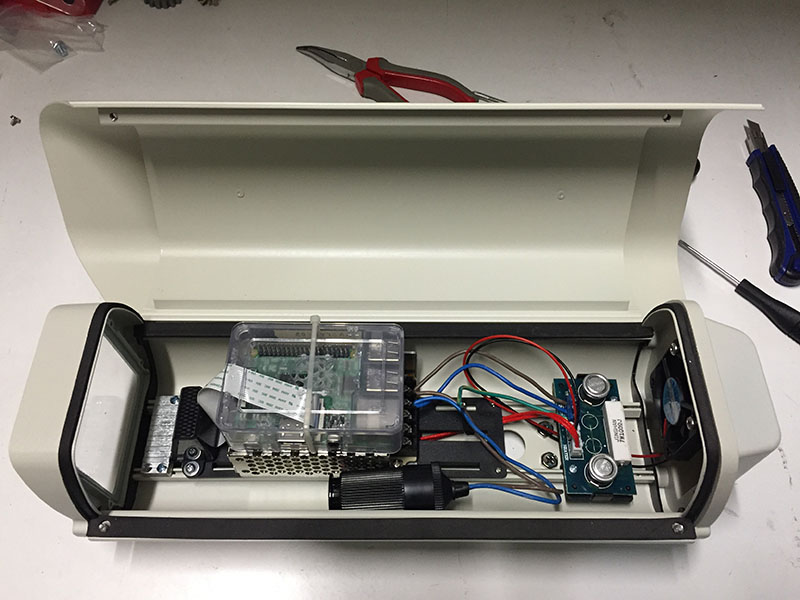
\includegraphics[width=\columnwidth]{camera_inside}
        \caption{Inside of a camera box}
	\end{subfigure} %
    \begin{subfigure}{0.48\columnwidth}
		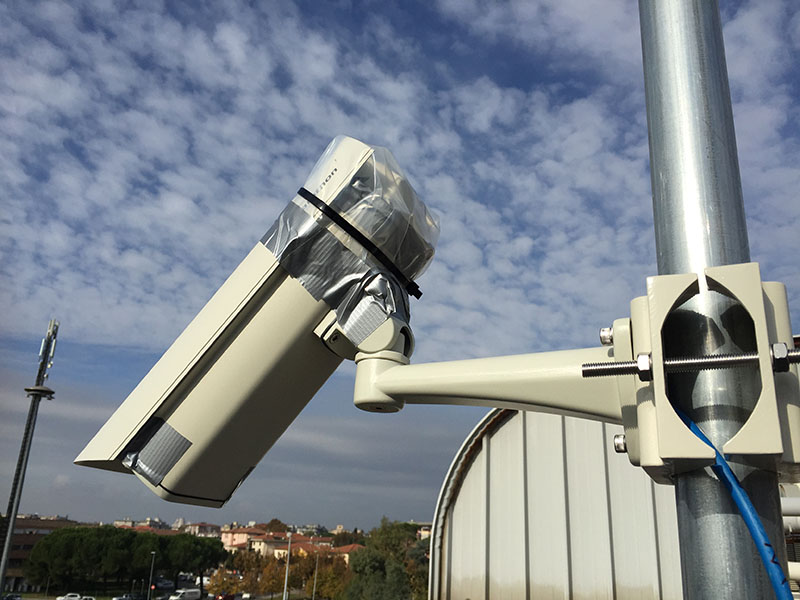
\includegraphics[width=\columnwidth]{camera_box}
        \caption{The complete camera box}
	\end{subfigure}

	\caption{Each Raspberry Pi is mounted inside a outdoor camera box (Figure $A$ on the left) and it is mounted on top of the roof of the building, attached to a steel pole (Figure $B$ on the right)}
	\label{fig:mini:camera-box}
\end{figure}

\begin{figure}
	\centering
		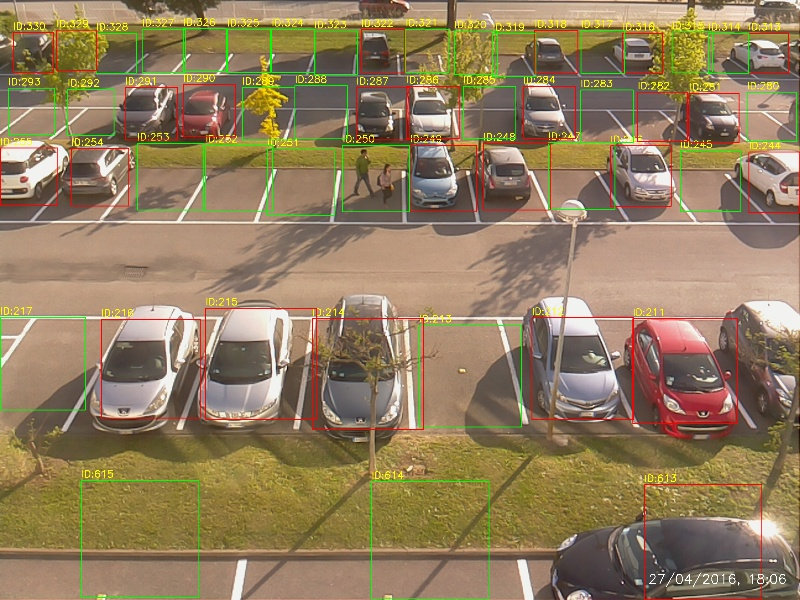
\includegraphics[width=\columnwidth,trim={0 0 0 3.5ex},clip]{detection-example}
        \caption{Example of classification of a portion of the parking lot}
	\label{fig:mini:detection-example}
\end{figure}

In this section, we describe the details of the deployment of a prototype of our proposed solution for parking lot visual occupancy detection in the campus of the National Research Council (CNR) in Pisa.

We deployed 9 smart cameras on the roof of the building in front of a section of the campus parking lot.
Each smart camera is built from a Rasbperry Pi 2 model B equipped with standard Raspberry Pi camera module and mounted on an outdoor camera box (see \ref{fig:mini:camera-box}).
The total cost for a single camera is roughly 80\euro.
Hardware and software details are briefly reported for completeness.
The smart cameras are equipped with an ARM Cortex-A7 CPU, 1GB RAM DDR2, and a 32GB micro SD card for storage.
The camera module is a 5MP fixed-focus camera that supports 1080p30, 720p60 and VGA90 video modes, as well as still captures.
The view angles of the camera are 53.50$^{\circ}$ horizontally and 41.41$^{\circ}$ vertically.
We capture still pictures at a full-sensor resolution of $2592 \times 1944$ pixels.
We used the OpenCV\footnote{http://opencv.org/} library to elaborate the frames acquired by the cameras, and Caffe \cite{jia2014caffe} to train and use neural networks.

Periodically, cameras capture an image of a portion of the parking lot, segment individual slots using manually defined masks, and determine the occupancy status for each slot using the \gls{cnn} trained off-line.
\ref{fig:mini:detection-example} shows an example of the occupancy detection performed by one camera in which common challenging aspects --- such as shadows, obstacles (trees or lamps) or even people occupying the parking slots --- are correctly managed.
In total, the cameras monitor 164 parking spaces organized in five rows, the first comprised by 18 parking spaces each, and the others by 35 parking slots each.
The number of parking slots monitored by each camera spans from 20 to more than 50, roughly, depending on the position of the parking slots with respect to the building on which cameras are mounted.
In fact, some cameras are dedicated to monitor most of the parking spaces closest to the building, while further spaces are monitored by multiple cameras.
We exploit the redundancy offered by multiple cameras to reduce the classification uncertainty when possible.
We combine the predictions of slots monitored by more than one camera by manually assigning weights to each (slot, camera) couple that represent the quality of the camera view for that particular slot.
As correct prediction for a slot, we take the one with highest weighted confidence.

The predicted occupancy status for each slot is submitted to a server for visualization and counting purposes.

% A key aspect of the proposed system is its decentralized approach
% and the delegation of the parking decision to the smart cameras
% themselves. This solution has the clear advantage of being scalable
% as it requires no additional elaboration on the server side. In a
% centralized solution images of the parking at high resolution (of
% about 3MB) should be sent to the server which would thus become a
% bottleneck and a single point of failure. Moreover, the network may
% be easily congested with increasing number of parking lots to be monitored.

\section{Conclusions}
\label{sec:mini:conclusions}

We proposed and evaluated a reduced \acrlong{cnn} architecture for image classification that enables smart vision applications in embedded devices.
In the scope of visual parking lot occupancy detection, we defined \emph{mAlexNet}, a reduced version of the famous \emph{AlexNet} classifier, which is obtained by pruning layers and reducing the number of parameters of the original architecture.
Experiments on public datasets shown that our proposed architecture outperforms state-of-the-art approaches for visual parking lot occupancy detection based on shallow models and hand-crafted features while requiring a computational budget suitable for embedded devices.
Specifically, our architecture exhibits very high accuracies even in presence of challenging light conditions variation, shadows, and partial occlusions.
Moreover, multi-dataset experiments shown that the architectural reduction does not introduce a performance degradation in real scenarios, and it produces only a slight acceptable degradation of the generalization capability, i.e.\ the ability of classifying images coming from different parking lots with different imaging conditions.

We tested our approach on a real scenario in the parking lot of the campus of the CNR Area in Pisa.
We deployed a decentralized system comprised by 9 smart cameras which monitors multiple slots and perform the occupancy detection for each slot on board.
The delegation of parking slot occupancy detection to smart cameras provides a twofold advantage.
First, with a cost of a single camera (roughly 80\euro), we are able to monitor at most 50 slots in our configuration, drastically reducing the cost per single slot that is nearly 100\euro for magnetic ground sensors while maintaining the same level of accuracy;
Second, the decentralized nature of our solution enables a higher degree of scalability, since there is no need of a central server to analyze images and a high bandwidth to transfer them.
In addition, the flexibility of the infrastructure does not limit the applications only to occupancy detection;
the spare computational resources can be used to perform other analyses such as video surveillance activities.

As a further contribution, we collected and made publicly available \emph{CNRPark-EXT}, a dataset containing images of a real parking lot taken by nine smart cameras, in different days, with different weather and light conditions.
\emph{CNRPark-EXT} covers a high variability of occlusions, point of views, light and weather conditions, which we experimentally demonstrated being of significant importance for the robustenss and generalization of occupancy detection systems.
This makes the dataset more compatible with real scenarios of outdoor parking lots, and represents a good complement to other publicly available datasets, for more reliable assessments.

%==========================

% Thanks to the use of deep CNN, the proposed solution is robust to disturbances created by partial occlusions, by the presence of shadows and by the variation of light conditions. % TODO integrate
% Moreover, it exhibits a good generalization property: in fact, the quality of the results is maintained when we consider parking lots and scenarios significantly different from the ones used during the CNN training phase.

%==========================

% \emph{mLeNet} is based on LeNet-5, proposed by \cite{lecun1998gradient}, having two convolutional layers followed by max pooling and two fully connected layers.
% The first layer (\emph{conv1}) is similar to the one proposed by \cite{krizhevsky2012imagenet} to be more suitable for a 224x224x3 input image.
% Layers \emph{conv2} and \emph{fc4} have a reduced number of filters and neurons with respect to \cite{lecun1998gradient} to better suit a binary classification task without overfitting.
% For \emph{fc5}, the last Gaussian RBF (radial basis function) layer is replaced with a classical inner product layer and a 2-way soft max classifier.

% Unlike \cite{krizhevsky2012imagenet} and \cite{lecun1998gradient}, both  architectures have a dense connection between convolutional layers.

% We used the Caffe framework \cite{jia2014caffe} to train the neural network and to initialize the classifier.

% We first compared the two proposed CNN architectures to select the one that offers the best performance.
% Afterwards, we compared our approach against other state-of-the-art methods.
% Finally, we performed experiments to analyze the difference between our CNN architecture.

% \subsection{Assessment of the Proposed CNNs}

% \noindent In order to assess the performance of the two CNN architectures
% \emph{mAlexNet} and \emph{mLeNet}, presented in Section
% \ref{sec:occupancy-detection}, we performed experiments using the
% \emph{CNRPark} dataset, considering two possible application
% scenarios:
% % a \emph{single camera scenario}, in which train and test data come from the same viewpoint, and
% % a \emph{multiple camera scenario}, in which training data and test data come from
% % different viewpoints.
% %
% \begin{inparaenum}[\itshape a\upshape)]
%   \item \emph{single camera scenario}, in which train and test data come from
%   the same viewpoint,
%   \item \emph{multiple camera scenario}, in which train data and
%   test data come from different viewpoints.
% \end{inparaenum}

% %Experiments are performed offline using the manually labeled data generated as
% %described in Subsection~\ref{sec:dataset}.
% Images of parking spaces are divided in two subsets,
% \emph{CNRPark A} and \emph{CNRPark B}, containing images respectively taken from
% a camera with central view and a camera with a side view of the parking lots
% (Figure~\ref{fig:cameraoverview}). Details are reported in
% Table~\ref{tbl:datasets}. All patches are shuffled and resized to a fixed size
% of 256x256 pixels. No information about the previous classification of a space
% is used to classify the same or other spaces, hence each image is classified
% independently from each other. For both the CNNs (mLeNet and mAlexNet), we
% perform a learning phase and a classification phase.

% For the single camera scenario, in order to limit problems of
% overfitting, we further divided the two subsets (\emph{CNRPark A}
% and \emph{CNRPark B}) considering independently odd numbered and
% even numbered spaces. Specifically, when we train on odd numbered
% we test on even numbered, and viceversa, for a total of eight
% experiments. This scenario allowed us to test the robustness of
% the proposed solution to possible changes that may occur during
% outdoor monitoring with fixed cameras, such as illumination
% changes, shadows and partial occlusions.

% For the multi camera scenario, we train both networks on an entire subset and
% then we test them on the other subset, for a total of four experiments. We tested
% the robustness of the proposed solution to viewpoint variations, allowing us to
% measure the ability of the solution to transfer the learned knowledge to a new
% unseen scenario.

% Training images are randomly cropped to 224x224 and randomly flipped
% horizontally, while for test images the central 224x224 crop is taken.
% We train our CNN models using the Caffe framework \cite{jia2014caffe} with
% gradient descend with momentum. The following hyper-parameters are used:
% momentum $0.9$; weight decay $5\cdot10^{-4}$. The initial learning rates are
% chosen independently for each experiment and they are reported in
% Table~\ref{tbl:cnn-experiments} (\emph{base lr} column). The learning rate is
% decreased two times by a factor 10 when the loss stabilizes, or after at most 10
% epochs, resulting in at most 30 epochs of training.
% Trained models are available for
% download.\footnote{http://claudiotest.isti.cnr.it/CNRPark/models/}

% \newcommand{\maxf}[1]{{\cellcolor[gray]{0.8}}#1}
% \begin{table}
%   \newcolumntype{Y}{>{\centering\arraybackslash}X}
%   \def\arraystretch{1.2}
%   \begin{tabularx}{\linewidth}{|Y|Y|Y|Y|Y|}
%     % \begin{tabular}{|c|c|c|c|c|}
%     % \hline
%     \multicolumn{5}{c}{\bfseries SINGLE CAMERA EXPERIMENTS} \\ \hline
%     \hline
%     \emph{train}            & \emph{test}             & \emph{net}    & \emph{base lr} & \emph{accuracy} \\ \hline
%     \multirow{2}{*}{A (even)} & \multirow{2}{*}{A (odd)}  & mLeNet          & 0.001            & 0.993             \\ \cline{3-5}
%                               &                           & \maxf{mAlexNet} & \maxf{0.01}      & \maxf{0.996}      \\ \hline
%     \multirow{2}{*}{A (odd)}  & \multirow{2}{*}{A (even)} & mLeNet          & 0.001            & 0.982             \\ \cline{3-5}
%                               &                           & \maxf{mAlexNet} & \maxf{0.005}     & \maxf{0.993}      \\ \hline
%     \multirow{2}{*}{B (even)} & \multirow{2}{*}{B (odd)}  & mLeNet          & 0.001            & 0.861             \\ \cline{3-5}
%                               &                           & \maxf{mAlexNet} & \maxf{0.01}      & \maxf{0.911}      \\ \hline
%     \multirow{2}{*}{B (odd)}  & \multirow{2}{*}{B (even)} & mLeNet          & 0.001            & 0.893             \\ \cline{3-5}
%                               &                           & \maxf{mAlexNet} & \maxf{0.005}     & \maxf{0.898}      \\ \hline
%   \end{tabularx}\\[2ex]
%   \begin{tabularx}{\linewidth}{|Y|Y|Y|Y|Y|}
%     % \hline
%     \multicolumn{5}{c}{\bfseries MULTI CAMERA EXPERIMENTS} \\ \hline
%     \hline
%     \emph{train}            & \emph{test}             & \emph{net}    & \emph{base lr} & \emph{accuracy} \\ \hline
%     \multirow{2}{*}{A}        & \multirow{2}{*}{B}        & mLeNet          & 0.0001           & 0.843             \\ \cline{3-5}
%                               &                           & \maxf{mAlexNet} & \maxf{0.001}     & \maxf{0.863}      \\ \hline
%     \multirow{2}{*}{B}        & \multirow{2}{*}{A}        & mLeNet          & 0.001            & 0.842             \\ \cline{3-5}
%                               &                           & \maxf{mAlexNet} & \maxf{0.0005}    & \maxf{0.907}      \\ \hline

%   \end{tabularx}
%   \vspace{1ex}
%   \caption{Settings and results of experiments performed on subsets $A$ and $B$
%   of \emph{CNRPark}, captured from different cameras. The even/odd
%   indication tells whether training or testing is performed only on images of
%   even or odd numbered spaces of that particular subset.}
%   \label{tbl:cnn-experiments}
% \end{table}

% \subsubsection{Results}

% \noindent The accuracy obtained at the end of the learning phase is reported
% in Table~\ref{tbl:cnn-experiments} for each configuration.

% Both CNNs, when tested in the single camera scenario, perform
% better on the subset \emph{CNRPark A}, which contains less
% occlusions and in which there are less variations between parking
% spaces. In fact, \emph{mAlexNet} reaches an accuracy of $0.996$
% in \emph{CNRPark A}. However, very good results are also obtained
% on subset \emph{CNRPark B}, where \emph{mAlexNet} reaches an
% accuracy of $0.911$, despite the very skewed viewpoint and the
% higher number of obstacles in the field of view. For the multi
% camera scenario, higher values of accuracy are obtained when
% training on the more complex subset \emph{CNRPark B}, from which
% the model can extract richer information and better generalize. In
% this case, \emph{mAlexNet} reaches an accuracy of $0.907$.

% In all configurations \emph{mAlexNet} offers the best
% performance, thanks to the use of a larger model that always
% boosts accuracy, although more effort is required to train it.


% \begin{figure*}[t]
%    \centering
%    \subfigure[]{\includegraphics[width=0.48\textwidth]{camera-a-output.jpg}}\qquad
%     \subfigure[]{\includegraphics[width=0.48\textwidth]{camera-b-output.jpg}}
%    \caption{\textsc{Output }}
%    \label{fig:output}
%\end{figure*}

% ===========

%\subsection{Multi-dataset experiments}

% We performed two types of comparative experiments using both
% \emph{CNRPark} and \emph{PKLot} datasets: \emph{intra-dataset}
% experiments and \emph{inter-dataset} experiments.

% With \emph{intra-dataset} experiments, we evaluated both
% techniques using, individually, one of the two dataset for both
% training and testing purposes. In this way, we estimated the
% performance of both techniques when the statistics of both train
% and test sets are similar.

% With \emph{inter-dataset} experiments, we used one of the two
% datasets to train and fine-tune each method, and we used the other
% dataset to test them. Hence, we estimated the ability of both
% techniques to generalize from the particular statistics of the
% training dataset.

% For more details about these experiments, see \cite{cnr.isti2015-TR-0402015}.


% For \emph{intra-dataset} experiments, both datasets have been
% divided into two partitions. \emph{CNRPark} has been divided in
% \emph{CNRParkEven}, containing images of even-numbered spaces,
% and \emph{CNRParkOdd}, containing images of odd-numbered spaces.\newline
% Both partitions have been used as training set and test set.
% \emph{PKLot} dataset has been divided in \emph{PKLot2Days} and
% \emph{PKLotNot2Days}. The former is formed choosing for each
% camera and for each weather condition the images of the first
% two days in chronological order, and the latter contains the
% remaining images. This partition strategy has been adopted to
% reduce training time, since only the smaller partition
% (\emph{PKLot2Days}) is used as training set.

% For \emph{inter-dataset} experiments, we trained on \emph{PKLot2Days} instead
% of using the whole \emph{PKLot} to reduce training times. Tests are however
% performed on the whole dataset.

% All the details of the datasets are reported in Table~\ref{tbl:datasets}, and
% results of performed experiments are summarized in
% Table~\ref{tbl:intra-inter-experiments}.

% In the \emph{intra-dataset} experiments, our method is
% comparable with the ones proposed in \cite{de2015pklot}.
% Using the highest confidence as classification output (having a
% threshold of $0.5$), the \emph{mAlexNet} achieves slightly higher
% accuracy values with respect to the other methods.

% In the \emph{inter-dataset} experiments, our method demonstrates
% a higher level of generalization, outperforming the other tested
% methods, achieving significantly higher accuracy values.

% \begin{table}
% 	\scriptsize
% 	\newcolumntype{Y}{>{\centering\arraybackslash}X}
% 	\newcolumntype{N}{S[table-format=1.2,round-mode=places,round-precision=2]}
% 	%\def\arraystretch{1.1}
% 	\begin{tabularx}{\linewidth}{|Y|N|N|N||N|N|}
% 		\multicolumn{4}{c}{\bfseries INTRA-DATASET} & \multicolumn{2}{c}{\bfseries INTER-DATASET}\\ \hline
% 		\textbf{train} & \multicolumn{1}{c|}{PKLot2Days}    & \multicolumn{1}{c|}{CNRParkOdd}  & \multicolumn{1}{c||}{CNRParkEven} & \multicolumn{1}{c|}{PKLot2Days} & \multicolumn{1}{c|}{CNRPark} \\
% 		\textbf{test}  & \multicolumn{1}{c|}{PKLotNot2Days} & \multicolumn{1}{c|}{CNRParkEven} & \multicolumn{1}{c||}{CNRParkOdd}  & \multicolumn{1}{c|}{CNRPark}    & \multicolumn{1}{c|}{PKLot}   \\ \cline{1-1}
% 		\textbf{model} &                                    &                                  &                                   &                                 &                              \\ \hline

% 		mAlex          & \maxf{0.981411554126166}           & \maxf{0.901312591152163}         & \maxf{0.907063776703571}          & \maxf{0.828830260648443}        & \maxf{0.903750400561001}     \\ \hline
% 		LPQu           & 0.965874918839068                  & 0.869227029654837                & 0.814907219709964                 & 0.646376350921806               & 0.398238824886945            \\ \hline
% 		LPQgd          & 0.970236471449698                  & 0.876519202722411                & 0.812880087322626                 & 0.617371265098538               & 0.409933050629474            \\ \hline
% 		LPQg           & 0.956938043299657                  & 0.868740884783666                & 0.816466552315609                 & 0.638350286077559               & 0.438087998402067            \\ \hline
% 		LBPuri         & 0.874336554245814                  & 0.850105331388754                & 0.763137377202557                 & 0.653051493960585               & 0.497392581394714            \\ \hline
% 		LBPu           & 0.950955664993196                  & 0.868416788202885                & 0.800249493216903                 & 0.642720915448188               & 0.466701346028662            \\ \hline
% 		LBPri          & 0.878793824909347                  & 0.864851725814293                & 0.819585217526899                 & 0.642005721551176               & 0.487172707533708            \\ \hline
% 		LBP            & 0.944891926341768                  & 0.874088478366553                & 0.872134726337128                 & 0.631277813095995               & 0.528790815908630            \\ \hline
% 	\end{tabularx}\\[5ex]

% 	\caption{Settings of \emph{intra-} and \emph{inter-dataset} experiments and achieved accuracy values.}
% 	\label{tbl:intra-inter-experiments}
% \end{table}

% For the comparisons, we evaluated the performance of the trained
% classifiers on the test sets measuring the accuracy and the Area
% Under the Curve (AUC) of Receiver Operating Characteristic (ROC)
% curves. ROC curves show how True Positive Rate (TPR), on y-axis,
% and False Positive Rate (FPR), on x-axis, vary as its score
% threshold is varied. AUC measures how much a curve leans near the
% perfect classification point, that is the point (0,1) on the ROC
% plot. AUC values range from 0 (perfect misclassification) to 1
% (perfect classification), where 0.5 indicates a classifier that
% performs like the random guessing classifier.

% \subsubsection{Results}

% In Figure~\ref{fig:roc-curves}, we report the ROC curves generated by
% each method tested on both datasets, and for convenience, in
% Table~\ref{tbl:intra-inter-experiments} we separately report the
% achieved accuracies.

% In the \emph{intra-dataset} experiments, our method is
% comparable with the ones proposed in \cite{de2015pklot} in terms
% of AUC. In fact, our \emph{mAlexNet} method reaches AUCs of
% $0.943$ on \emph{CNRParkEven}, $0.920$ on \emph{CNRParkOdd},
% and $0.996$ on \emph{PKLotNot2Days}, which are very close to
% respectively $0.957$, $0.923$, and $0.997$ of the best performing
% compared methods, as can be seen in Figure~\ref{fig:roc-curves}.

% Using the highest confidence as classification output (having a
% theshold of $0.5$), the \emph{mAlexNet} achieves slightly higher
% accuracy values with respect to the other methods. In fact, we reach
% and accuracy of $0.901$ on \emph{CNRParkEven}, $0.907$ on
% \emph{CNRParkOdd}, and $0.981$ on \emph{PKLotNot2Days}, which are
% higher than respectively $0.877$, $0.872$, and $0.970$ of the best
% performing compared methods, as can be seen in
% Table~\ref{tbl:intra-inter-experiments}.

% In the \emph{inter-dataset} experiments, our method demonstrates
% a higher level of generalization, outperforming the other tested
% methods. In fact, the \emph{mAlexNet} method reaches AUCs of
% $0.899$ on \emph{CNRPark}, and $0.989$ on \emph{PKLot}, which
% are definitively better than respectively $0.580$, and $0.743$, of
% the best performing compared methods, as can be seen still in
% Figure~\ref{fig:roc-curves}.

% Hence, the same situation goes for accuracy values when using $0.5$ as threshold,
% \emph{mAlexNet} achieves significantly higher accuracy values.
% In fact, as can be seen in Table~\ref{tbl:intra-inter-experiments},
% we reach and accuracy of $0.829$ on \emph{CNRPark}, and $0.904$
% on \emph{PKLot}, versus respectively $0.646$, and $0.529$, of
% the best performing compared methods.

% \usepackage{graphics} is needed for \includegraphics
% \begin{figure*}[htp]
%   \begin{center}
%     \begin{minipage}[t]{.495\textwidth}
%       \centering
%       \includegraphics[width=.9\linewidth]{eval/ROC-classify-CNRParkEven-train-on-CNRParkOdd}\\[3ex]
%       \includegraphics[width=.9\linewidth]{eval/ROC-classify-CNRParkOdd-train-on-CNRParkEven}\\[3ex]
%       \includegraphics[width=.9\linewidth]{eval/ROC-classify-PKLotNot2Days-train-on-PKLot2Days}
%     \end{minipage} \hfill
%     \begin{minipage}[t]{.495\textwidth}
%       \includegraphics[width=.9\linewidth]{eval/ROC-classify-CNRPark-train-on-PKLot2Days}\\[3ex]
%       \includegraphics[width=.95\linewidth]{eval/ROC-classify-PKLot-train-on-CNRPark}\\[3ex]
%       \caption{ROC curves for intra-dataset (left column) and inter-dataset
%       (right column) experiments, where the positive class is `busy'.
%       Methods in the legends are sorted by descending values of AUC.}
%       \label{fig:roc-curves}
%     \end{minipage}
%   \end{center}
% \end{figure*}

%===================== CROSS-MEDIA LEARNING FOR IMAGE CLASSIFIERS =========================

\graphicspath{{img/vsa/}}

\newcommand{\BTSA}{B-T4SA}
\newcommand{\ourFtAlex}{Hybrid-T4SA}
\newcommand{\ourFtVGG}{VGG-T4SA}

\chapter{Weakly-supervised Cross-media Learning of Convolutional Neural Networks}
\label{ch:cross-media}

The most straightforward way to build a visual image classifier using \glspl{cnn} is to perform supervised learning.
While in previous work the cost of human interaction was spent on the manual engineering of features detectors and descriptors, this cost recently shifted to the labeling of datasets in order to train deep models.
Even if the labeling task is simpler and more accessible, correctly labeling huge datasets is still a labor-intensive and expensive job, which is usually carried out by crowd-sourcing.
Current large-scale datasets, such as ImageNet, are in fact limited in their scalability due to the labeling cost on which their collectors incur.
Thus, the attention of recent research shifted to the exploitation of the huge amount of data coming from the web and social media which became easily available in the last years~\cite{sun2017revisiting,mahajan2018exploring}.
The main objective is to reduce the amount of human interaction needed to train an image classifier and obtain good features by exploiting correlation that can emerge in large-scale datasets.
Despite having the advantage of being free and constantly growing, this source of data poses challenges in its usage, since it commonly presents noisy or incomplete information.
This usually limits the amount of supervision that can be extracted from this kind of data, but the possibility to scale the training procedures to a huge amount of data often compensates this limitation.

In this chapter, we propose a novel weakly-supervised cross-media approach to train visual image classifiers in an autonomous way exploiting social media data.
We rely on textual data --- which usually accompanies images in social media posts --- to provide a noisy supervision in the training phase of a visual-only classifier.
To exhibit the advantages of our approach, we employed it to tackle \emph{\gls{vsa}} --- a problem in which the cost of data labeling is rather high --- using a \acrfull{dcnn} trained without hand-assigned ground-truth.
We present an empirical study to analyze visual sentiments in the wild, starting from a large-scale dataset of \emph{unlabeled} user-generated content.
To the best of our knowledge, this is the first work that proposes a cross-media approach to learn a classifier for predicting the sentiment polarity of a given image.
We demonstrate via experimental evaluation on existing manually-labeled benchmarks that models trained with our approach are able to extensively exploit the noisy information contained in uncontrolled social media data to build a visual sentiment polarity classifier with no human supervision that outperforms state-of-the-art classifiers trained on sentiment-related labeled images.
Overall, we collect and analyze more than 3 million tweets from which we build \emph{\acrfull{t4sa}} --- a dataset of about 1 million high-confidence tweets, for which we provide the textual sentiment classification, and the corresponding 1.4M images.
We make all the collected tweets, the \gls{t4sa} dataset, and trained models publicly available to foster new research on the field of visual sentiment analysis.

The chapter is structured as follows.
In \ref{sec:vsa:introduction}, the problem of visual sentiment analysis is presented, together with a discussion about the challenges it poses and an overview of the current state of the art.
\ref{subsec:vsa:dataset} presents the methodology used to collect and preprocess the social media data used in our experiments.
In \ref{subsec:vsa:method}, our weakly-supervised cross-media learning approach is described in detail, and \ref{sec:vsa:experiments} reports its experimental evaluation and comparison with state-of-the-art approaches to visual sentiment analysis.
\ref{sec:vsa:conclusion} summarizes the main findings and concludes the chapter.

The research presented in this chapter was published in~\cite{vadicamo2017cross}, and the provided resources --- e.g., datasets and trained models --- are available at \url{http://t4sa.it}.


%%% ABSTRACT
% Much progress has been made in the field of sentiment analysis in the past years. Researchers relied on textual data for this task, while only recently they have started investigating approaches to predict sentiments from multimedia content.
%With the increasing amount of data shared on social media, there is also a rapidly growing interest in approaches that work ``in the wild'', i.e., that are able to deal with uncontrolled conditions.
%In this work, we faced the challenge of training a visual sentiment classifier starting from a large set of user-generated and unlabeled contents.
%In particular, we collected more than 3 million tweets containing both text and images, and we leveraged on the sentiment polarity of the textual contents to train a visual sentiment classifier.
%To the best of our knowledge, this is the first time that a cross-media learning approach is proposed and tested in this context.
%We assessed the validity of our model by conducting comparative studies and evaluations on a benchmark for visual sentiment analysis.
%Our empirical study shows that --- although the text associated to each image is often noisy and weakly correlated with the image content --- it can be profitably exploited to train a deep Convolutional Neural Network that effectively predicts the sentiment polarity of previously unseen images.

\section{Visual Sentiment Analysis}
\label{sec:vsa:introduction}

Recent years experienced a rapid and increasing adoption of social media as information exchange and communication platforms.
On a daily basis, users generate and share a large quantity of multimedia content --- such as texts, images, and videos --- which conveys information about their opinions about a vast range of topics.
The availability of such a source of data attracted the scientific community as well as the industries to large-scale sentimental analyses of the public opinion.
Opinion mining and sentiment analysis~\cite{pang2008opinion} foster applications in multiple domains, such as market prediction~\cite{mishne2006predicting,asur2010predicting}, government intelligence~\cite{abbasi2007affect}, political elections~\cite{laver2003extracting,o2010tweets}, and crisis management~\cite{avvenuti2016impromptu,cresci2015linguistically}, to name a few.

Thanks to the multi-modality of modern social platforms, current trends show that visual media are increasingly chosen due to their immediate and effective communication, and less and less text is written by users.
Therefore, researchers shifted their attention from a pure textual-based sentiment analysis presented in seminal work to a multi-modal analysis which includes also visual information conveyed by images and videos~\cite{borth2013large,cao2016cross,jou2015visual,siersdorfer2010analyzing,you2015robust,you2016cross}.
In particular, we identify as \emph{visual sentiment analysis} the task of extracting subjective information --- such as emotions and opinions --- solely from visual data.
Understanding the content of a piece of visual information is an objective task, and much progress has been made in the computer vision research community to accurately describe visual contents, i.e., reducing the semantic gap between image representations and content~\cite{li2016socializing}.
However, describing the emotions arisen in human observers is challenging due to the high subjectivity involved.
This discrepancy between the affective content of an image and its description --- known as the \emph{affective gap}~\cite{siersdorfer2010analyzing} --- poses considerable challenges to visual sentiment analysis.
This difficulty is also reflected in the generation of labeled sets for training sentiment classifiers;
several emotional judgments by multiple annotators are usually required to obtain a high-quality sentiment ground-truth for a single image, thus increasing the cost of dataset creation.

While in general sentiment analyses can tailor a large range of emotions, the commonly adopted form of sentiment analysis is the determination of the sentiment polarity of a piece of information, i.e., an indicator of the emotional positiveness or negativeness conveyed.
This formulation is often sufficient for most sentiment analysis applications while simplifying the problem to be solved.
As the vast majority of attempts in the literature, we adopt the same formulation in our work;
thus, our goal is to predict the sentiment polarity of a given image.
In the next paragraphs, we will provide the reader with an overview of existing work on sentiment analysis with emphasis on the ones based on visual data.

\paragraph{Text-based Sentiment Analysis}
%For what concerns the detection of sentiment polarity in texts extracted from Twitter, first works considered simple linguistic features, such as word unigrams, word bigrams and parts-of-speech, using machine learning algorithms like Naive Bayes, Maximum Entropy and \acrfullpl{svm}.
Seminal works on sentiment polarity estimation from textual data~\cite{go2009twitter,bermingham2010classifying} employed classic \gls{ml} algorithms which relied on simple linguistic features --- such as word n-grams and part-of-speech.
%In the last few years, deep neural networks contributed to considerable performance improvements with respect to other popular learning algorithms, such as \glspl{svm}.
Subsequently, deep learning approaches positively contributed with more accurate models for text analysis and natural language processing, which in turn gave a huge contribution in textual sentiment analysis.
%In particular, \acrfullpl{lstm}, which we also employ in this work, and \acrfullpl{cnn} were tested on several shared tasks, such as the Semeval Sentiment analysis in Twitter \cite{nakov2016semeval}, which is considered by the Natural Language Processing community the most important benchmark for this task.
%The results obtained by the submitted systems, such as the ones by \citet{deriu2016swisscheese} and \citet{rouvier2016sensei}, have shown that the combination of these learning techniques with the adoption of word embeddings, a compact real-value vector word representation which takes into account word similarity \cite{mikolov2013distributed,pennington2014glove}, is able to set the state-of-the-art with minimal feature engineering, which makes such architectures more robust and flexible than previous ones.
The Semeval Sentiment analysis in Twitter \cite{nakov2016semeval} challenge is a testimony of this influence: an increasing number of submitted solutions~\cite{deriu2016swisscheese,rouvier2016sensei} combined the power of deep models --- such as \acrfullpl{lstm} and \acrfullpl{cnn} --- and word embeddings~\cite{mikolov2013distributed,pennington2014glove} to set the state of the art with minimal or no feature engineering.

% ---

\paragraph{Visual Sentiment Analisys}
In comparison to textual-based sentiment analysis, inferring emotional information from visual content has been less explored by the research community.
Seminal approaches \cite{machajdik2010affective,siersdorfer2010analyzing,jia2012can} relied on supervised or semi-supervised frameworks that map low-level features of images into human emotions.
\citet{siersdorfer2010analyzing} firstly applied and evaluated automatic classification of the sentiment using a large-scale collection of photos crawled from Flickr using the SentiWordNet \cite{esuli2007sentiwordnet} dictionary as query terms.
They used a pixel-level color histogram and \gls{sift}-based \acrlong{bow} representations as visual features and trained a \gls{svm} to predict the sentiment of images.
% To overcome the \emph{affective gap} between low-level features and the emotional content of an image,  employed visual entities or attributes to extract mid-level visual representations.
% The main contribution of~\cite{borth2013large} and~\cite{jou2015visual} was building a large scale visual sentiment ontology, called VSO and Multilingual VSO, respectively, which consist of thousands of semantic objects (Adjective Noun Pairs -- ANP) strongly linked to emotions.
% Using their ontologies, they also proposed a bank of detectors, namely \emph{SentiBank} and \emph{MVSO}, that can automatically extract these mid-level representations.
Subsequent works \cite{borth2013large,yuan2013sentribute,jou2015visual} proposed to employ large-scale sentiment ontologies --- like VSO~\cite{borth2013large} or MVSO~\cite{jou2015visual} --- comprised by emotion-related concepts identified by adjective-noun pairs.
%For example, Sentibank detects the responses of 1200 ANP concepts in an image, which means that it represents each image by a 1200-dimensional vector of responses.
%For the sentiment prediction task, a classifier is learned on the top of these mid-level representations that are used as image features.
Ontologies are used to build a feature extractor --- called \emph{SentiBank} --- which creates a mid-level visual representation based on the visual detection of these concepts, on which in turn the sentiment prediction relies.
%\citet{chen2014deepsentibank} proposed an improved version of SentiBank, called \emph{DeepSentiBank} which exploit \acrfullpl{dcnn} to build a visual sentiment concept classification model.
\citet{chen2014deepsentibank} extended this approach proposing \emph{DeepSentiBank}, in which the concept detection is carried out by deep convolutional models.
%Following the success of deep learning, many other approaches based on deep neural networks have been proposed for visual sentiment prediction and image emotion classification \cite{campos2017pixels,chen2014deepsentibank,islam2016visual,rao2016learning,you2015robust,xu2014visual}.
Many other approaches employed \glspl{dcnn} for visual sentiment prediction and image emotion classification~\cite{campos2017pixels,chen2014deepsentibank,islam2016visual,rao2016learning,you2015robust,xu2014visual}.
% ---
Most of these have in common the use of \glspl{cnn} trained or fine-tuned on sentiment-related and labeled data.
In \cite{campos2017pixels,chen2014deepsentibank,islam2016visual,jou2015visual}, %,xu2014visual %sun2016discovering %VGGNet \cite{simonyan2014very}
state-of-the-art \gls{cnn} architectures --- such as AlexNet~\cite{krizhevsky2012imagenet}, PlaceCNN~\cite{zhou2014learning}, and GoogleNet \cite{szegedy2015going} --- were exploited.
\citet{you2015robust} proposed a custom \gls{cnn} architecture specifically designed for visual sentiment prediction.
Since their network was trained on weakly labeled images, they also proposed an approach, called PCNN, to reduce the impact of noisy training images. %instances by progressively select a subset of the training images.
\citet{sun2016discovering} boosted the performance of CNNs by selecting affective local regions of the images which are likely containing objects and carrying massive emotions. % NOELAB
% This means that the ANP's textual sentiments are not explicitly used for the sentiment prediction.
Just recently, \citet{li2018image} investigated the fusion of the sentiment prediction obtained using visual ontologies with the sentiment prediction obtained using the textual sentiment values of adjective-noun pairs on which ontologies are built.


\paragraph{Multi-modal Sentiment Analysis}
There are also several publications on analyzing sentiments using multi-modalities, such as text and image.
For example, \citet{cao2016cross} proposed a late fusion to combine the predictions obtained from text and image, while \citet{you2016cross} proposed a cross-modality consistent regression (CCR) scheme for joint textual and visual analysis.
Recently, multi-modal learning approaches have been proposed for joint textual and visual understanding.
\citet{baecchi2016multimodal} proposed a multi-modal feature learning schema based on CBOW and denoising autoencoders to perform sentiment analysis.
In \cite{mao2014deep}, the authors proposed a deep end-to-end architecture where each modality is encoded is an appropriate sub-network (an \gls{rnn} for text and a \gls{cnn} for images) and then fused in a multi-modal layer.
Similarly, \citet{ma2015multimodal} encodes both modalities with convolutional networks.

Differently from all the approaches previously presented, in our work we are interested in i) understanding human sentiments by exploiting a large-scale dataset of unlabeled images collected from social-media, ii) training sentiment classifiers without any prior knowledge of the collected data.
Although textual information accompanying social media images is often incomplete and noisy, it can be effectively exploited to enable unsupervised sentiment analysis.
A first step in this direction was taken in \cite{wang2015unsupervised} where an Unsupervised SEntiment Analysis (USEA) for social-media images based on nonnegative matrix factorization was proposed.
Our work differs from that of \citet{wang2015unsupervised} in the way of exploiting the textual information and in the final classifier.
In fact, we train a deep neural network that can be used to predict the sentiment of any new image \emph{without} using any textual information for those images, while USEA infers sentiments for images by \emph{jointly} considering visual and textual information.
%Moreover, Wang \etal  did not test their approach on hand-labeled images or benchmarks for visual sentiment analysis for further comparisons.

%-------------------------------------------------------------------------

\section{Learning Visual Sentiment Classifiers}

We focus our investigation on training a model to predict the sentiment polarity of a given image.
We formulate this task as learning a three-way image classifier that can assign either \emph{positive}, \emph{negative} or \emph{neutral} label to an image.
As other state-of-the-art approaches, we exploit deep learning models to build our visual sentiment classifiers.
However, differently from previous supervised approaches, we propose an end-to-end pipeline to train the visual classifier starting from a large-scale dataset of unlabeled tweets.
As source of multi-modal information, we choose Twitter, from which we crawled tweets from the random stream of global tweets with a minimum set of restriction.
We exploit the correspondence of text and images present in tweets to distill affective information from the textual modality to the visual one.
In particular, we use a pre-trained textual predictor --- based on a tandem \gls{LSTM}-\gls{SVM} architecture --- to infer the sentiment polarity from the textual part of a tweet
Then, we transfer this sentiment polarity to the images attached to the same tweet, obtaining a dataset of labeled images we can use as training set to fine-tune \glspl{dcnn} architectures for the task of visual sentiment polarity prediction.
Although the text of the tweets is often noisy or misleading with respect to the image content (e.g., irrelevant comments), we show that our cross-media approach can be profitably used for learning visual sentiment classifiers in the wild.
At test time, the trained \glspl{dcnn} can be used to infer the sentiment polarity of an image without the need of textual data.

In the next sections, we will describe the data collection process, the pre-trained textual sentiment classifier which provides us with weak supervision, and the training process of visual models.
%An overview of our approach is depicted in \ref{fig:vsa:overview}.
% TODO [FIGURE] VSA overview
%\begin{figure}
%    \centering
%    \includegraphics{}
%    \caption{.}
%    \label{fig:vsa:overview}
%\end{figure}

% We follow the current trend of facing sentiment ``in the wild", that is, in all sort of varying conditions of the everyday world that we share with others (as opposed to testing situation in laboratories).
% For this scope, social networks, such as Twitter and Facebook, are particularly suitable as sources of data for our analysis, thanks to the huge variation of contents shared by their users.

%-------------------------------------------------------------------------

\subsection{Data Collection}
\label{subsec:vsa:dataset}
Both the textual and the multimedia data used in this work have been collected from Twitter, by means of a streaming crawler.
The data collection process took place from July to December 2016, lasting around 6 months in total.
During this time span, we exploited Twitter's Sample API\footnote{https://dev.twitter.com/streaming/reference/get/statuses/sample} to access a random 1\% sample of the stream of all globally produced tweets.
All the tweets collected undergone a filtering step in order to retain only data that could be useful for our sentiment analysis task.
Specifically, we discarded: i) retweets; ii) tweets not containing any static image (i.e., we also discarded tweets containing only videos and/or animated GIFs); iii) tweets not written in the English language; iv) tweets whose text was less than 5 words long.
This ensures that we collect tweets with both images and text, and that there is enough textual data for the textual sentiment classification task.
Discarding retweets avoids collecting large numbers of duplicated images.
The above set of rules filtered as much as 98.7\% of all the tweets collected from the Twitter stream.
Anyway, the huge volume of tweets produced globally still allowed to collect a stream of more than 43 useful tweets per minute, on average.
At the end of the data collection process, the total number of tweets in our dataset is roughly 3.4M, corresponding to roughly 4M images.
Then, we classified the sentiment polarity of the \emph{texts} as described in the next section, and we selected the tweets having the most confident textual sentiment predictions to build our \emph{\acrfull{t4sa}} dataset.
\gls{t4sa} contains little less than a million tweets, corresponding to roughly 1.5M images.
We publicly release all the collected tweets and the \gls{t4sa} dataset.

%-------------------------------------------------------------------------

\subsection{Inferring Sentiment Polarity from Text}
\label{subsec:vsa:method}

The text extracted from the collected tweets has been classified according to the sentiment polarity using an adapted version for the English language of the ItaliaNLP Sentiment Polarity Classifier~\cite{cimino2016tandem}.
This system was successfully employed in the SENTIment POLarity Classification task~\cite{barbieri2016overview}, which was organized within Evalita 2016, the 5th evaluation campaign of Natural Language Processing and Speech tools for Italian.
This classifier is based on a tandem LSTM-SVM architecture.
\gls{svm} classifiers usually rely on ``sparse" and ``discrete" features in document classification tasks, making difficult the detection of relationships in sentences, which is often the key factor in detecting the overall sentiment polarity in documents~\cite{tang2015document}.
On the contrary, \glspl{lstm} was recently tested on Sentiment Analysis and proved to outperform previous systems \cite{nakov2016semeval} thanks to their ability to capture long-term dependencies sentences.
In the tandem architecture, \glspl{lstm} learn the feature space and capture temporal dependencies between words, while \glspl{svm} are used for the final classification.
\glspl{svm} combine the document embedding produced by the \gls{lstm} with a wide set of general-purpose features qualifying the lexical and grammatical structure of the text.
In particular, the system employs a bidirectional \gls{lstm} architecture due to their ability to capture long-range dependencies analyzing the text in both directions~\cite{schuster1997bidirectional}.

The tandem system in trained in two steps.
First, the \gls{lstm} network is trained for sentiment analysis classification on a three-way label space (\emph{positive}, \emph{neutral}, or \emph{negative}).
Once the statistical model of the \gls{lstm} is fitted, for each document of the training set, a document vector (document embedding) is computed extracting the activation of the penultimate layer (the one before the classifier).
The document embeddings, together with manually defined document features, are used to train a \gls{svm} classifier .
Once the training phase of the \gls{svm} classifier is completed, the tandem architecture is considered trained.
The same stages are involved in the classification phase: for each document, the \gls{lstm} is used to obtain an embedding vector which is used jointly with other document classification features (see Section \ref{exp:visual} for further details) by the \gls{svm} classifier which outputs the predicted class.

The textual sentiment classifier has been evaluated by means of a 10-fold cross validation over 6,293 tweets belonging to the dataset distributed for the SemEval-2013 Task on Sentiment Analysis in Twitter.
Using the subset of approximately 60\% of the original dataset which was still available, the textual classifier reported an average $F_1$-score of $66.15$.
This result is comparable to the state of the art considering that the winner of the competition, the NRC-Canada team \cite{mohammad2013nrc}, achieved an $F_1$-score of 69.02 using all the available training data.

We used the tandem \gls{lstm}-\gls{svm} model to analyze the text of the large set of user-generated tweets collected.
After predicting the sentiment polarity of all the tweets, we selected the ones having the most confident textual sentiment predictions using a threshold, and we used these predictions to automatically assign sentiment labels to the corresponding images.
The set of tweets and images retained after this step comprise our \gls{t4sa} dataset.
% The aim was to automatically build a training set for learning a \emph{visual} classifier able to discover the sentiment polarity of a given image.
%The text analysis have been used to build our dataset \gls{t4sa} by selecting tweets with the most confident textual sentiment predictions.

% ---

We modeled this task as a three-way image classification problem in which each image can be classified as either \emph{positive}, \emph{neutral}, or \emph{negative}.
To build our visual classifier, we leveraged on transfer learning, i.e., we fine-tune known and successful deep CNNs architectures pre-trained on generic datasets of images.
Doing so, we are able to exploit additional knowledge already stored in the trained network while training for sentiment prediction.
Thus, we initialize the weights of layers with the ones of the pre-trained networks, except for the last layer that produces the sentiment classification, which is randomly initialized.
We used a balanced subset of our dataset \gls{t4sa} to perform fine-tuning.

As \gls{cnn} architecture, we tested \emph{HybridNet}~\cite{zhou2014learning} and \emph{VGG-19}~\cite{simonyan2014very} models.
The architecture of \emph{HybridNet} is the same of the \emph{BVLC Reference CaffeNet}~\cite{jia2014caffe}, which mimics the original AlexNet \cite{krizhevsky2012imagenet} with minor variations as described in~\cite{zhou2014learning}.
The model --- comprised by $5$ convolutional and $2$ fully-connected layers --- is pre-trained on $1,183$ categories ($205$ scene categories from Places205~\cite{zhou2014learning} and $978$ object categories from the train data of ImageNet~\cite{russakovsky2015imagenet}) with about $3.6$ million images.
The \emph{VGG-19} is an improved version of the model used by the \gls{vgg} team of the University of Oxford in the ILSVRC-2014 competition, as described in \cite{simonyan2014very}.
The model is pre-trained on $1,000$ categories of ImageNet~\cite{russakovsky2015imagenet} with about $1.5$ million images.
It contains $19$ learnable layers; $16$ convolutional and $3$ fully-connected.
% %________________________________________________________
% Both the pre-trained models can be downloaded from the \emph{Caffe Mode Zoo} \footnote{\url{http://caffe.berkeleyvision.org/model_zoo.html}}.
% In \ref{exp:visual}, we describe the fine-tuning process used for building our visual sentiment classifiers.

%-------------------------------------------------------------------------
\section{Experimental Evaluation}
\label{sec:vsa:experiments}

In this section, we will describe the experimental protocol we followed respectively to prepare our data, train our visual sentiment classifiers, and compare them against state-of-the-art approaches on standard benchmarks.

\subsection{Dataset Preparation}

All the $\sim$3.4M tweets collected as reported in \ref{subsec:vsa:dataset} are analyzed by the textual sentiment polarity classifier described in \ref{subsec:vsa:method}.
In order to produce a reliable dataset for learning a visual sentiment classifier, we selected only the tweets classified with a confidence $\geqslant 0.85$.
We used as threhold the value achieving state of the art in textual sentiment classification challenge with an $F$-score of $0.71$.
The resulting dataset contains $371,341$ positive, $629,566$ neutral, and $31,327$ negative labeled tweets.
As expected, the dataset proved to be very imbalanced, a frequent and known issue in social media sentiment data \cite{li2011semi}.
In order to increase the number of negative tweets, we selected a lower filtering threshold for this class, obtaining $179,050$ examples.
Notably, in our experiments conducted on \gls{t4sa}, the difference in precision on the classification of positive, neutral, and negative never exceeds $1\%$; thus, the lower threshold used for selecting negative examples did not impact the quality of the learning.
Starting from this dataset, we selected a balanced subset of images to train visual sentiment classifiers.
To do so, we performed the following steps: i) we labeled each image of \gls{t4sa} on the basis of the corresponding textual sentiment classification; ii) we removed corrupted and near-duplicate images resulting in $\sim$ 974K unique images; iii) we selected a \emph{balanced} subset composed by $156,862$ images for each class, resulting in a set of $470,586$ images named \BTSA{}; iv) we split {\BTSA} in training, validation and test subsets, corresponding approximately to 80\%, 10\%, and 10\% of the images.

\begin{table}
\centering
\newcolumntype{R}{>{\raggedleft\arraybackslash}X}
\begin{tabularx}{\linewidth}{lRRRR}
\toprule
                    & \multicolumn{2}{c}{\textsc{T4SA}} & \textsc{T4SA} {\footnotesize (no dup.)} & \textsc{B-T4SA} \\
                      \cmidrule(lr){2-3}                  \cmidrule(lr){4-4}      \cmidrule(lr){5-5}
\textsc{Sentiment}  & \textbf{tweets} & \textbf{images} & \textbf{images}       & \textbf{images} \\
\midrule
Positive            &  371,341        &   501,037       & 372,904               & 156,862 \\
Neutral             &  629,566        &   757,895       & 444,287               & 156,862 \\
Negative            &  179,050        &   214,462       & 156,862               & 156,862 \\
\midrule
Sum                 &  904,395        & 1,473,394       & 974,053               & 470,586 \\
\bottomrule
\end{tabularx}
\caption{Our \acrfull{t4sa} dataset and its subsets used for learning our visual classifiers. Each tweet (text and associated images) is labeled according to the sentiment polarity of the text, predicted by our tandem LSTM-SVM architecture.}
\label{tab:vsa:t4sa}
\end{table}

Details on \gls{t4sa} and its subsets are summarized in \ref{tab:vsa:t4sa}.
Notice that the size of the balanced subset (i.e., {\BTSA}) is highly influenced by the low number of tweets classified as negative.
Moreover, these negatives contain many artificial images --- such as screenshots and memes --- which made our analysis more challenging.
In fact, we encountered difficulties in automatically collecting negative tweets that also contain natural images by using only a random sample of all globally produced tweets.
However, in order to avoid possible biases in our analyses, we deliberately avoided to use any keyword during the data collection process.

%-----------------------------------------------------------------------------
\subsection{Experimental Settings}
\label{exp:visual}

% TODO quanta di questa roba è già nel paper loro?? inutile riportare tanta roba qua..
\paragraph{Text Analysis Settings}
As described in \ref{subsec:vsa:method}, we employed a bidirectional \gls{lstm} to learn a document embedding into a feature space.
For training, we applied a dropout factor of $0.45$ to both input gates and to the recurrent connections in order to prevent  overfitting~\cite{gal2016theoretically}.
A cross-entropy loss is employed and optimized by means of the \emph{rmsprop} optimizer \cite{tieleman2012lecture}.
% We used the Keras \cite{libkeras} deep learning framework to develop the \gls{lstm} network.

Each input word to the \gls{lstm} is represented by a low dimensional, continuous and real-valued vector, also known as word embedding~\cite{mikolov2013distributed}, and all the word vectors are stacked in a word embedding matrix.
For this work, we used GloVe~\cite{pennington2014glove} pre-trained vectors. % since these are computed considering the word context information.
GloVe website~\footnotetext{http://nlp.stanford.edu/projects/glove/} provides freely available pre-trained vectors computed from a 2B English tweets corpus.

The document embedding produced by the \gls{lstm} is used in conjunction with other document features by the \gls{svm} classifier.
The other document features focused on a wide set of features ranging across different levels of linguistic description.
The features are organised into three main  categories: raw  and  lexical  text  features, morpho-syntactic features and lexicon features.
With the exception of the lexicon features, these features were already tested and described in~\cite{cimino2016tandem}.
To extract the lexicon features we exploited three freely available resources: The Bing Liu Lexicon~\cite{hu2004mining}, which includes approximately 6,000 English words, the Multi-Perspective Question Answering Subjectivity Lexicon~\cite{wilson2005recognizing}, which consists of approximately 8,200 English words, and the SentiWordNet 3.0 Lexicon~\cite{baccianella2010sentiwordnet} that consists of more than 117,000 words.
For each word in these lexicons the associated polarity is provided.
In addition, we manually developed a lexicon of positive and negative emoticons, which are usually a strong indicator of the tweet sentiment polarity.
By exploiting the described resources, the following features were extracted: positive/negative emoticon distribution, sentiment polarity n-grams, sentiment polarity modifiers, the distribution of sentiment polarity, the most frequent sentiment polarity, and changes of polarity in tweet sections.
The last lexicon feature is calculated using the word embedding produced by GloVe, and it is obtained by computing separately the average of the word embeddings of the nouns, adjectives, and verbs of the tweet.

\paragraph{Image Analysis Settings}
We used the training subset of \BTSA{} to fine-tune the two pre-trained \glspl{cnn}, HybridNet and VGG-19\footnote{Both the pre-trained models can be downloaded from the \emph{Caffe Mode Zoo} (\url{http://caffe.berkeleyvision.org/model_zoo.html})}.
We replaced the last fully connected layer \emph{fc8} with a new one having 3 outputs, and we experimented two different fine-tuning strategies we named \emph{FT-F} and \emph{FT-A}.
In \emph{FT-A}, we fine-tune all the trainable layers, while in \emph{FT-F} the parameters of convolutional layers are fixed, and only the last fully connected layers \emph{fc6-8} are trained.
%In \emph{FT-C} we keep the first three convolutional layer fixed (or the first three groups of convolutions for the VGG-19) and we finetune layers from \emph{conv4} to the end of the networks.

We trained both networks with both the fine-tune strategies using Caffe \cite{jia2014caffe}for $15$ epochs using SGD with momentum $\mu = 0.9$, a learning rate of $0.001$ divided by $10$ every $5$ epochs, and L2 regularization with a weight decay of $10^{-5}$.
For HybridNet, we used a batch size of $128$, while for VGG-19 we used a batch size of $32$ with batch accumulation of $2$ to lower the GPU memory footprint.

We assessed the performance of our models using \BTSA{} test set and \acrfull{ttd}~\cite{you2015robust}.
The latter contains a total of $1,269$ images manually labeled with a positive or negative sentiment by manually by five Amazon Mechanical Turk (AMT) workers.
The images are partitioned into three subsets, namely ``Five agree", ``At least four agree", and ``At least three agree", on the basis of the labeling results from the five AMT workers.
The details of this dataset are reported in \ref{tab:vsa:ttd}.
\gls{ttd} was also used in \cite{campos2017pixels,islam2016visual,li2018image,you2015robust}, allowing for a through comparison of our systems with the state-of-the-art approaches.

\begin{table}
\centering
\newcolumntype{R}{>{\raggedleft\arraybackslash}X}
\begin{tabularx}{\linewidth}{lRRR}
\toprule
                   & \multicolumn{3}{c}{\textsc{Twitter Testing Dataset}} \\
                     \cmidrule(lr){2-4}
\textsc{Sentiment} & \textbf{5 agree} & \textbf{$\mathbf{\geq 4}$ agree} & \textbf{$\mathbf{\geq 3}$ agree} \\
\midrule
Positive           & 581              & 689                              & 769   \\
Negative           & 301              & 427                              & 500   \\
\midrule
Total              & 882              & 1,116                            & 1,269 \\
\bottomrule
\end{tabularx}
\caption{Twitter Testing Dataset \cite{you2015robust}.}
\label{tab:vsa:ttd}
\end{table}

\subsection{Results}
In \ref{tab:vsa:results}, we reported the accuracy obtained by the fine-tuned models in our \BTSA{} test set and in all the subsets provided by the \acrlong{ttd}.
\begin{table}
    \centering
    \newcolumntype{R}{>{\raggedleft\arraybackslash}X}
    \begin{tabularx}{\linewidth}{lRRRR}
    \toprule
                                & \multicolumn{3}{c}{\textsc{Twitter Testing Dataset}} & \multicolumn{1}{c}{\textsc{B-T4SA TEST}} \\
                                & \multicolumn{3}{c}{{\small (pos, neg)}}              & \multicolumn{1}{c}{{\small (pos, neu, neg)}} \\
                                  \cmidrule(lr){2-4}                                     \cmidrule(lr){5-5}
    \textsc{Model}              & \textbf{5 agree} & \textbf{$\mathbf{\geq 4}$ agree} & \textbf{$\mathbf{\geq 3}$ agree} & \\
    \midrule
    Random Classifier           & 0.500 & 0.500 & 0.500 & 0.333 \\
    CNN~\cite{you2015robust}    & 0.722 & 0.686 & 0.667 & -     \\
    PCNN~\cite{you2015robust}   & 0.747 & 0.714 & 0.687 & -     \\
    \ourFtAlex\, FT-F           & 0.766 & 0.748 & 0.723 & 0.499 \\
    \ourFtAlex\, FT-A           & 0.741 & 0.709 & 0.686 & 0.491 \\
    \ourFtVGG\, FT-F            & 0.768 & 0.737 & 0.715 & 0.506 \\
    \ourFtVGG\, FT-A            & \textbf{0.785} & \textbf{0.755} & \textbf{0.725} & \textbf{0.513} \\
    \bottomrule
    \end{tabularx}
	\caption{Prediction accuracy on the different test sets.}
    \label{tab:vsa:results}
\end{table}
As baseline references, we report the results obtained by the random classifier and by the CNN and PCNN models \cite{you2015robust}.
The results show that the models trained with our cross-media approach effectively classify the images of \gls{ttd} which were manually annotated.
In particular, our best model ({\ourFtVGG} FT-A) correctly classifies $78.5\%$ of the \emph{five agree} testing images, outperforming similar models trained on high-quality sentiment-related hand-labeled data~\cite{you2015robust}.
Since \gls{ttd} only provides binary labels (positive/negative) as ground-truth, we obtained a binary classification from our three-way model taking the maximum confidence between the positive and the negative confidences.
We also performed experiments using two-way fine-tuned nets trained only on positives and negatives images provided by our training set, but we observed that there is no significant difference in performance with respect to predictions derived from three-way models.
% Moreover, despite the presence of noisy labels especially for negative training images, our best model obtain similar F1 scores for both the positive (0.83) and negative (0.72) classes, meaning that is not too much biased towards a particular class.

Notice that the range of the accuracy values obtained on our \BTSA{} is lower because those experiments concern a three-way classification.
Moreover, the ground-truth for the evaluation is not hand-labeled since it is derived from the analysis of the textual information collected ``in the wild";
thus it contains noisy labels that inevitably lower the accuracy upper bound. %(see Figure \ref{fig:confusion-images}).
\ref{fig:vsa:confusion-images} reports the most confident classifications on this test set.
From a qualitative point of view, in several cases the sentiment polarity of the images is better represented by the prediction of our model than the sentiment polarity inferred from the text associated with the images.
Since the textual sentiment analysis was used to label both testing and training images, this, on one hand, explains the relatively lower accuracy obtained by our models on the \BTSA{} test set and, on the other hand, confirms that we used sufficiently large set of training data to allow the deep neural network to handle noisy labels.
Moreover, we observed that the use of the \emph{neutral} class is particularly suitable for analyzing web images, which often depict simple objects or commercial products.
For this reason we used a three-way model, unlike other state-of-the-art approaches which use a binary classification model~\cite{campos2017pixels,islam2016visual,you2015robust}.

% Many papers on visual sentiment analysis also report the 5-fold cross-validation accuracy on the Twitter Testing Dataset \cite{Campos2016,islam2016visual,li2018image,you2015robust}, in which the prediction of each fold is computed with a model fine-tuned on the other four folds. This measure tends to highlight how well a pretrained model adapts to a specific task or dataset. While we think that this measure is inappropriate for our cross-media approach, we also report it in Table \ref{tab:Twitter882_5fold} for comparison with other state-of-the-art methods.
% As evidenced by the results, the 5-fold accuracy of models trained on generic (not sentiment-related) datasets, like AlexNet and VGG-19, are comparable to the ones of the same models that have been previously finetuned on a sentiment-related dataset.

\begin{figure}
\centering
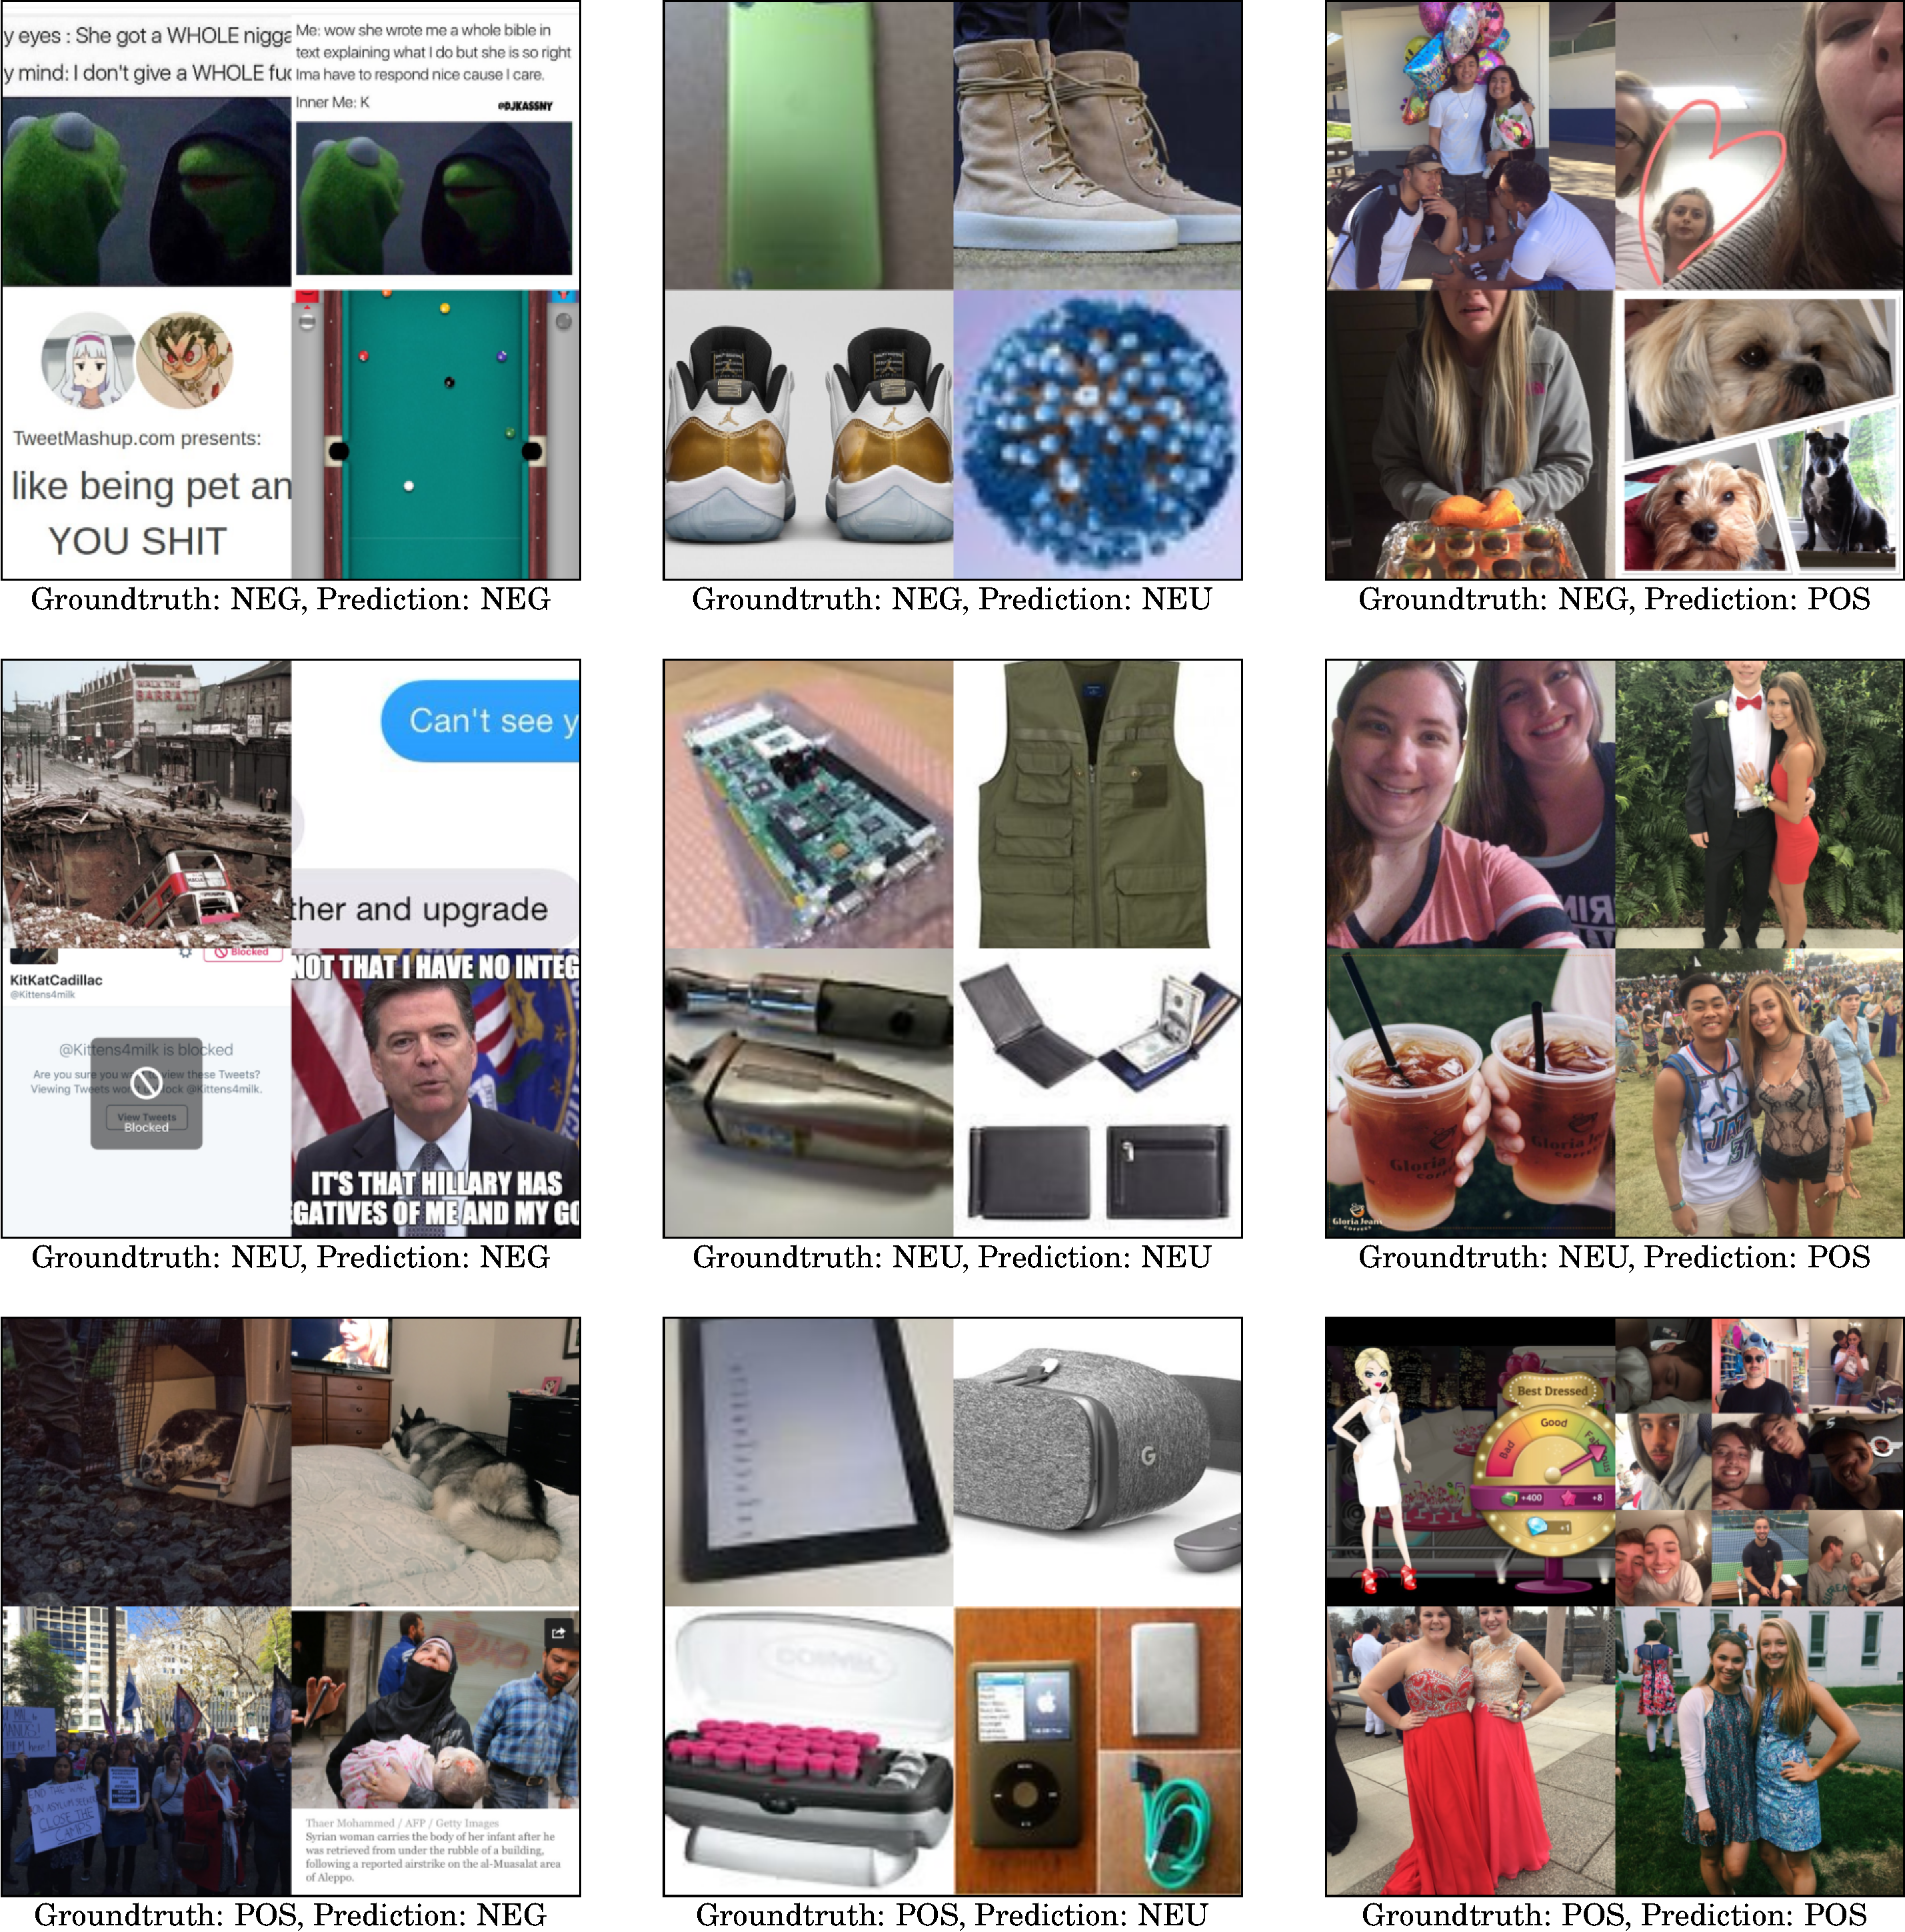
\includegraphics[width=\linewidth]{confusion-images}
\caption{The most confident classifications of our model on our \BTSA\, test set, grouped by all possible (ground-truth, predicted class) couples. Rows (from top to bottom) contains images labeled respectively \emph{negative}, \emph{neutral} and \emph{positive} on the basis of textual sentiment analysis. Columns (from left to right) contain images visually classified respectively as \emph{negative}, \emph{neutral} and \emph{positive} by our model.
%From a qualitative point of view, notice that in several cases the sentiment polarity of the images is better represented by the prediction of our model than the sentiment polarity inferred from the text associated to the images. Since the textual sentiment analysis was used to label both testing and training images, this, on one hand, explains the low accuracy upper bound obtained by our model on the {\BTSA} test set and, on the other hand, confirms that we used sufficiently large set of training data to allow the deep network to handle noisy labels.
}
\label{fig:vsa:confusion-images}
\end{figure}

A considerable amount of works on visual sentiment analysis report the 5-fold cross-validation accuracy on the Twitter Testing Dataset~\cite{campos2017pixels,islam2016visual,li2018image,you2015robust}, in which the prediction of each fold is computed with a model fine-tuned on the other four folds.
In order to compare to those approaches, we also tested our models in this setting, and we reported the 5-fold accuracy obtained in \ref{tab:vsa:fold-results}.
However, we think that this measure is inappropriate for our cross-media approach since it tends to highlight how well a pre-trained model adapts to a specific task or dataset.
In fact, as evidenced by the results, models trained on generic (not sentiment-related) datasets, like AlexNet and VGG-19, not necessarily perform worse than the same models previously fine-tuned on a sentiment-related dataset.
For example our best approach ({\ourFtVGG} FT-A), achieves a 5-fold accuracy of $0.896$ on the five agree subset, that corresponds only to an improvement of $1.5\%$ with respect to VGG-19 trained on a generic dataset.
Moreover, our technique is based on a cross-media approach, i.e., it relies on labels not coming from a visual inspection of the images.
Thus, we think that a fine-tuning of our models on manually labeled images is inappropriate for our goal.
In any case, also in this test setting, our models outperform other state-of-the-art visual classifiers, such as PCNN, DeepSentiBank and MVSO, which were trained on high-quality sentiment-related dataset.

Taken together, these results indicate that our cross-media learning approach is a first, important step towards building systems able to learn the sentiment polarity of images autonomously from the Web.

%Differently by other visual sentiment classifiers

% In order to compare the performance of our model to other state-of-the-art methods, we also performed a 5-fold cross-validation on the testing subsets (as also done in \cite{Campos2016,islam2016visual,li2018image,you2015robust}), in which we compute the prediction of each fold with a model fine-tuned again on the other four folds. Results for 5-fold cross-validation are reported in Table \ref{tab:Twitter882_5fold}.
\begin{table}
\small
\renewcommand{\tabcolsep}{2.7pt}
\newcolumntype{R}{>{\raggedleft\arraybackslash}X}
\begin{tabularx}{\linewidth}{llRRR}
\toprule
                &                           & \multicolumn{3}{c}{\textsc{Twitter Testing Dataset}} \\
                                              \cmidrule(lr){3-5}
\textsc{Method} & \textsc{Training Datasets} & \textbf{5 agree} & \textbf{$\mathbf{\geq 4}$ agree} & \textbf{$\mathbf{\geq 3}$ agree} \\
\midrule
\multicolumn{5}{l}{\textbf{Approaches without intermediate fine-tuning}} \\
\midrule
GCH~\cite{siersdorfer2010analyzing}              {\footnotesize (from~\cite{you2015robust})} $\ast$  &   -   &   0.684   &   0.665   &   0.66    \\
SentiBank~\cite{borth2013large}  {\footnotesize (from~\cite{you2015robust})} $\circ$ &   -   &   0.709   &   0.675   &   0.662   \\
LCH~\cite{siersdorfer2010analyzing}              {\footnotesize (from~\cite{you2015robust})} $\ast$  &   -   &   0.710   &   0.671   &   0.664   \\
GCH+ \gls{bow}~\cite{siersdorfer2010analyzing}         {\footnotesize (from~\cite{you2015robust})} $\ast$  &   -   &   0.710   &   0.685   &   0.665   \\
LCH+ \gls{bow} ~\cite{siersdorfer2010analyzing}        {\footnotesize (from~\cite{you2015robust})} $\ast$  &   -   &   0.717   &   0.697   &   0.664   \\
Sentribute~\cite{yuan2013sentribute}   {\footnotesize (from~\cite{you2015robust})} $\circ$ &   -   &   0.738   &   0.709   &   0.696   \\

CNN~\cite{you2015robust} $\bullet$   &   Flickr (VSO)    &   0.783   &   0.755   &   0.715   \\
AlexNet {\footnotesize (from~\cite{campos2017pixels})} $\bullet$   &  \gls{ilsvrc}12   &   0.817   &   0.782   &   0.739   \\
PlaceCNN~\cite{zhou2014learning}                {\footnotesize (from~\cite{campos2017pixels})} $\bullet$   &   Places205    &   0.830   &   -   &   -   \\
GoogleNet~\cite{szegedy2015going}   {\footnotesize (from~\cite{islam2016visual})}  $\bullet$   &   \gls{ilsvrc}12   &   0.861   &   0.807   &   0.787   \\
HybridNet $\bullet$   &   \gls{ilsvrc}12 + Places205   &   0.867   &   0.814   &   0.781   \\
VGG-19 $\bullet$   &   \gls{ilsvrc}12  &   0.881   &   0.835   &   0.800   \\

\midrule
\multicolumn{5}{l}{\textbf{Approaches using an intermediate fine-tuning}} \\
\midrule

PCNN~\cite{you2015robust} $\bullet$   &   Flickr (VSO) + \emph{ft} Flickr (VSO)  &   0.773   &   0.759   &   0.723   \\
DeepSentiBank~\cite{chen2014deepsentibank} {\footnotesize (from~\cite{campos2017pixels})} $\circ$ $\bullet$ &   \gls{ilsvrc}12 + \emph{ft} Flickr (VSO)  &   0.804   &   -   &   -   \\
MVSO [EN]~\cite{jou2015visual}   {\footnotesize (from~\cite{campos2017pixels})} $\circ$ $\bullet$ & DeepSentiBank~\cite{chen2014deepsentibank} + \emph{ft} MVSO-EN \cite{jou2015visual}  &   0.839   &   -   &   -   \\
\ourFtAlex\, FT-A (Ours) $\bullet$   &   (\gls{ilsvrc}12 + Places205) + \emph{ft} \BTSA    &   0.864   &   0.830   &   0.800   \\
\ourFtAlex\, FT-F (Ours) $\bullet$   &   (\gls{ilsvrc}12 + Places205) + \emph{ft} \BTSA   &   0.873   &   0.832   &   0.810   \\
\ourFtVGG\, FT-F (Ours) $\bullet$   &   (\gls{ilsvrc}12 + Places205) + \emph{ft} \BTSA   &   0.889   &   0.857   &   0.815   \\
\ourFtVGG\, FT-A (Ours) $\bullet$   &   (\gls{ilsvrc}12 + Places205) + \emph{ft} \BTSA &   \textbf{0.896   }&  \textbf{0.866}  &   \textbf{0.820}  \\

\midrule
\end{tabularx}
$\ast=$ based on low-level features, $\circ=$ based on mid-level features, $\bullet=$ based on deep learning
\footnotesize
%\item[$\ast$]  Approch based on low-level features
%\item[$\circ$]  Approch based on mid-level features
%\item[$\bullet$] Approch based on deep learning

\caption{5-Fold Cross-Validation Accuracy of different methods on Twitter Testing Dataset. \emph{tr} stands for `trained'; \emph{ft} stands for `fine-tuned'. Note that in these experiments \emph{all} the deep models are again fine-tuned on four folds of the Twitter Testing Dataset. During cross-validation we fine-tuned all the weights of our FT models.}
\label{tab:vsa:fold-results}
\end{table}

% \subsubsection{Results on Phototweet Sentiment Benchmark(?)} %LUCIA%rivedere il titolo e decidere se inserire gli exp
% \cite{borth2013large}
% Ground-truth obtained by AMT annotation

%-------------------------------------------------------------------------

\section{Conclusions}
\label{sec:vsa:conclusion}

In this chapter, we tackle the problem of reducing the cost of builing datasets for training deep models for image classification.
We proposed a fully automatic cross-media pipeline that builds a weakly-labeled dataset exploiting social media data and its multi-modality that can be used to train deep models drastically reducing the human interaction needed.
We apply our approach in the context of training a visual sentiment classifier from a large set of multimedia data, without the need of human annotators.
We leveraged on textual information associated to Web images --- which is often noisy and ambiguous --- and demonstrated it is still useful for learning robust visual classifiers.
To this scope, we collected and used more than 3 million tweets, and we experimentally shown that our approach is effective for learning visual sentiment classifier in the wild.
We publicly released all the collected data and our trained models for future research and applications.
%======================= ADVERSARIAL DETECTION IN DNN ===========================

\graphicspath{{img/adversarial/}}

\chapter{Adversarial Examples Detection in Deep Convolutional Image Classifiers}
\label{ch:adversarial}

%%% ABSTRACT
%
% Notwithstanding that, recent works have demonstrated that it is quite easy to create adversarial examples, i.e., images malevolently modified to cause deep neural networks to fail. Such images contain changes unnoticeable to the human eye but sufficient to mislead the network. This represents a serious threat for machine learning methods. In this paper, we investigate the robustness of the representations learned by the fooled neural network, analyzing the activations of its hidden layers.
% Specifically, we tested scoring approaches used for kNN classification, in order to distinguish between correctly classified authentic images and adversarial examples.
% These scores are obtained searching only between the very same images used for training the network.
% The results show that hidden layers activations can be used to reveal incorrect classifications caused by adversarial attacks.

As we can notice from the previous chapters, deep neural networks are more and more pervading an increasing number of computer vision applications.
Noteworthy applications not considered in this thesis include image tagging~\cite{li2016socializing}, video captioning~\cite{baraldi2016hierarchical}, face verification~\cite{schroff2015facenet,parkhi2015deep}, super resolution~\cite{dong2016image}, just to name a few.
As the spread of \gls{dl}-based solution increases, also its adoption in sensible applications --- such as image forensics \cite{tuama2016camera,bayar2016deep,zhang2016image,amerini2017localization}, spam/malware detection \cite{dahl2013large}, and self-driving cars \cite{cirecsan2012multi} --- increases accordingly.

Unfortunately, researchers shown that machine learning models, including deep learning methods, are highly vulnerable to adversarial examples~\cite{klarreich2016learning,goodfellow2014explaining,szegedy2013intriguing,papernot2016practical}.
An \emph{adversarial example} is a malicious input sample typically created applying a small but intentional perturbation such that the attacked model misclassifies it with high confidence \cite{goodfellow2014explaining}.
In most of the cases, the difference between the original and perturbed image is imperceptible to a human observer.
Moreover, adversarial examples created for a specific neural network have been shown to be able to
fool different models with different architecture and/or trained on similar but different data~\cite{szegedy2013intriguing,papernot2016practical}.
These properties are known as cross-model and cross-dataset generalization of adversarial examples and imply that adversarial examples pose a security risk even under a threat model where the attacker does not have access to the target's model definition, model parameters, or training set~\cite{papernot2016practical,kurakin2016adversarial}.

It becomes crucial to understand how adversarial actions are perpetrated in order to consequently build up solutions to be robust against such attacks.
Most of the effort of the research community in defending from adversarial attacks had gone into increasing the model robustness to adversarial examples via enhanced training strategies, such as adversarial training~\cite{goodfellow2014explaining,papernot2016limitations} or defensive distillation~\cite{papernot2016distillation,grosse2016adversarial}.
%Fast adversarial generation methods \cite{goodfellow2014explaining,papernot2016limitations} enable simple strategies such as adversarial training, that is the inclusion of adversarial examples generated on-the-fly in the training set.
%Other approaches \cite{papernot2016distillation,szegedy2013intriguing} suggest to reduce or mask the classifier's decision surface and reduce the magnitude of the gradients towards adversarial points an attacker would exploit, or even completely mask the gradients using non-differentiable classifiers, such as kNNs.
However, studies have shown~\cite{papernot2016practical} that those techniques only increase the cost of adversarial example generation without completely solving the problem.
% - till now research tried to train models which are robust to this type of attacks, while no much work on detecting adversarial images
A parallel strategy recenly studied is to defend from adversarial attacks by distinguishing adversarial inputs from authentic inputs.
% - our contribution

\begin{figure}
\centering
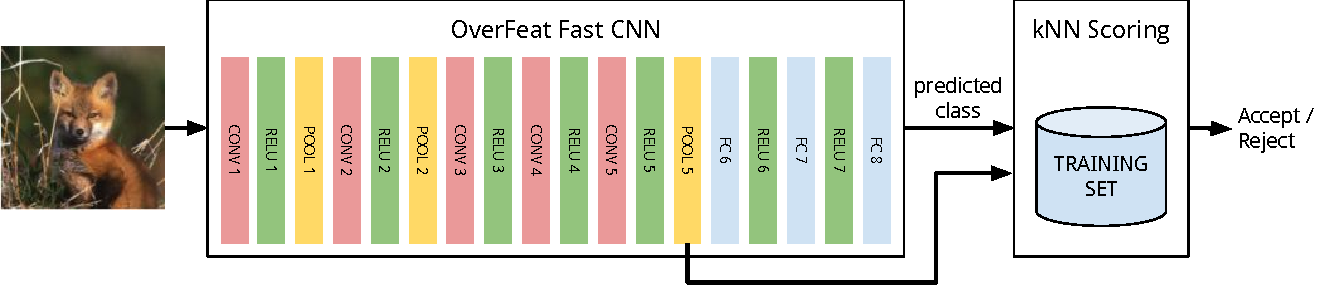
\includegraphics[width=\linewidth]{overview}
\caption{Overview of our detection approach. The input image is classified by the CNN, but we consider the classification valid only if the kNN score of the predicted class based on deep features (\emph{pool5}) is above a certain threshold.}
\label{fig:adv:overview}
\end{figure}

In this work, we present an approach to detect adversarial examples in deep neural networks based on the analysis of activations of the neurons in hidden layers --- also known as \emph{deep features} --- of the attacked neural network.
Being deep learning a subset of representation learning methods, we expect the learned representation to be more robust than the final classification to adversarial examples.
Moreover, adversarial images are generated in order to look similar to humans, and deep features have shown impressive results in visual similarity related tasks such as content-based image retrieval~\cite{sharif2014cnn,gordo2016deep}.
% Our main conjecture is the following,
% An authentic and its adversarial samples are almost identical at the input and produce very similar activations in the first layers of the network.
% Then, activations start diverging and produce completely different outputs.
% Our main conjecture is that we are able to tell adversarial samples from authentic ones looking at the intermediate activations of the network instead of its output.
Our investigation shows that, given an input image, searching for similar deep features among the images used for training allows us to predict the correctness of the classification produced by a \gls{dnn}.
In particular, we emply traditional kNN scoring approaches as a measure of the confidence of the classification given by the \gls{dnn}.
The score assigned by the kNN classifier to the class predicted by the \gls{dnn} is used as a confidence measure of the reliability of the predicted class.
The experiments show that we are able to filter out the majority of adversarial examples, while retaining most of the correctly classified authentic images.
The choice of the discriminative threshold is a trade-off between accepted false negatives (FN) and true positives (TP), where positive means non-adversarial.
%
% In this work, we present an approach to detect adversarial examples in deep neural networks, based on the similarity of intermediate network activations.
% Our main conjecture is the following.
% Since authentic and adversarial samples are very similar but activate the network in a very dissimilar way in the output layer, we should be able to discern the authentic samples from the adversarial ones looking at the network's intermediate activations.
% We show that kNN classifiers based on euclidean distances between intermediate layers' activations can be used to predict the correctness of the classification produced by a \gls{dnn}.
% In particular, the scores assigned by the kNN can be used as a measure of confidence on the predicted class.
% This allows to filter out many adversarial examples while retaining most of the correctly classified authentic images.

% For better understanding how an adversarial works, we'll start explaining briefly what is a Convolutional Network (because this model works well in visual tasks), then we'll describe what an adversarial example exploits to fool the classier and what happen in a ConvNet when this kind of image is given as input.

% This paper is and extended version of the work ``Detecting adversarial example attacks to deep neural networks'' by the same authors, submitted to the 2nd International Workshop on Multimedia Forensics and Security (MFSec 2017).
% In this version, we considered more hidden layers (\emph{pool5} and \emph{fc7}) and more kNN classification approaches (Weighted and Distance Weighted).
% We also added plots and a discussion about the cumulative distribution of scores (Figure \ref{fig:adv:score-densities}).

The chapter is structured as follows.
\ref{sec:adv:rel-work} reviews relevant work in the field of adversarial attacks and their analysis, and provides background knowledge about adversarial detection and generation algorithms.
In \ref{sec:adv:detection}, our approach to adversarial detection is presented, while in \ref{sec:adv:experiments} we describe the experimental settings we used to validate it.
Finally, \ref{sec:adv:conclusions} summarizes the main findings and presents some future research directions.

The research presented in this chapter was published in~\cite{carrara2017detecting,carrara2018adversarial}, and additional resources are available at \url{http://deepfeatures.org/adversarials/}.


\section{Adversarial Examples}
\label{sec:adv:rel-work}

One of the first works exploring adversarial examples for image classifiers implemented with convolutional neural network is the one of \citet{szegedy2013intriguing}.
The authors used a quasi-newtonian optimization method, namely L-BFGS, to find an image $\x_{adv}$ close to an original one $\x$ in terms of L2 distance, yet differently classified.
They also have shown that the obtained adversarial images were also affecting different models trained on the same training set (\emph{cross-model generalization}) and also models trained with other yet similar training sets (\emph{cross-training set generalization}).
Cross-model and cross-training set generalization properties of adversarial examples are also confirmed in \cite{tabacof2016exploring}, where the authors explored the pixel space around adversarial images moving in random directions applying different kinds of noise.
They show that adversarial images are not isolated, spurious points, but they occupy large regions of the pixel space that mislead models with similar classification boundaries.
While multipletheories has been proposed, the causes of the adversarial vulnerability of \gls{ml} models remain an open question.
Early explanations suggested that it is due to non-linearity of a deep neural networks and over-fitting \cite{tabacof2016exploring}, while \citet{goodfellow2014explaining} argued that the primary cause of neural networks' vulnerability to adversarial perturbation is their linear nature.
In particular, the alignment between adversarial perturbations and weights in a high-dimensional dot product can cause high spourious activations even if small perturbations are given as input.

% \paragraph{Crafting algorithms}
To overcome to the high computational cost of the L-BFGS approach, \citet{goodfellow2014explaining} also proposed the \gls{fgsm} to efficiently find adversarial perturbations following the gradient of the loss function with respect to the image, which can be efficiently computed by back-propagation.
Many other methods derived from \gls{fgsm} have been proposed to efficiently craft adversarial images.
\citet{kurakin2016adversarial} proposed a basic iterative version of \gls{fgsm} in which multiple finer steps are performed to better explore the adversarial space.
\citet{dong2018boosting} proposed a version of iterative \gls{fgsm} equipped with momentum which won the NIPS Adversarial Attacks and Defences Challenge~\cite{kurakin2018adversarial} as best attack;
this resulted in adversarial images with an improved transferability among models.
% attacks we did not test but relevant to the field
Other attack strategies aim to find smaller perturbations using a higher computational cost.
\citet{nguyen2015deep} used evolutionary algorithms and gradient ascent optimization to produce fooling images which are unrecognizable to human eyes but are classified with high confidence by \glspl{dnn}.
% \cite{papernot2016limitations} used forward derivatives to compute adversarial saliency maps that show which input feature have to be increased or decreased to produce the maximum perturbation of the last classification layer towards a chosen adversarial class.
% JSMA
In~\cite{papernot2016limitations}, a Jacobian-based saliency map is computed and used to greedily identify the best pixel to modify in order to steer the classification to the desired output.
% They also derived different metrics from adversarial saliency maps, such as \emph{hardness}, \emph{adversarial distance} and \emph{robustness}, to measure the ability of a model to cope with adversarial attacks.
% DeepFool
In~\cite{moosavi2016deepfool}, the classifier is locally linearized and a step toward the simplified classification boundary is taken, repeating the process until a true adversarial is reached.
% In \cite{moosavi2016universal}, Moosavi et al. presented an algorithm to find image-agnostic (universal) adversarial perturbations for a given trained model, that are able fool the classifier with high probability when added to any input. % The authors also observed that universal adversarial perturbations show cross-model and cross-dataset generalization properties.
% Carlini Wagner
\citet{carlini2016towards} relied on a modified formulation of the adversarial optimization problem initially formalized by \citet{szegedy2013intriguing}.
They move the misclassification constraint in the objective function by adding a specifically designed loss term, and they change the variable of the optimization to ensure the obtained image is valid without enforcing the box constraint;
\gls{adam} is then employed to optimize and find better adversarial perturbations.
\citet{sabour2015adversarial} explored the manipulation of a particular internal representation of the network by means of adversarial inputs, showing that it is possible to move the representation closer to the one of a provided guide image.
% Features Adversarial  % to bypass our detector you have to change the evolution of all the features, not just one.
\citet{papernot2016practical} also shown that successfully attacks are possible even if the attacker does not have direct access to the model weights or architecture.
In fact, the authors successfully performed adversarial attacks to remotely hosted models, and \citet{kurakin2016adversarial} also showed that attacks in physical scenarios, such as feeding a model with a printout adversarial example through a digital camera, are possible and effective.

% - defenses
\paragraph{Defensive Strategies}
In the recent literature, a considerable amount of work has been dedicated to increasing the robustness of the attacked models to adversarial inputs.
In \cite{szegedy2013intriguing}, the authors suggest to add a regularization term to the training loss based on the Lipschitz upper bound, that resembles a L2 regularization, to limit the magnitude of the changes in the activations of a network caused by perturbations of the input.
\citet{gu2014towards} shown that denoising autoencoders can remove substantial amounts of the adversarial noise.
However, when stacking the autoencoders with the original neural network, the resulting network can again be attacked by new adversarial examples with even smaller distortion.
Thus, the authors proposed Deep Contractive Network, a model with an end-to-end training procedure that includes a smoothness penalty.
Fast crafting algorithms, such as \gls{fgsm}, enabled a defensive strategy called \emph{adversarial training}, in which adversarial examples are generated on the fly and added to the training set while training~\cite{goodfellow2014explaining,huang2015learning}.
While models that undergo adversarial training still suffer from the presence of adversarial inputs, the perturbation needed to reach them is usually higher, resulting in a higher detectability.
However, easily optimizable models, such as models with non-saturating linear activations, can be easily fooled due to their overly confident linear responses to points that not occur in the training data distribution~\cite{goodfellow2014explaining}.
This concept is also discussed in~\cite{papernot2016towards}, where the authors shows that there are tensions between model accuracy and resilience that has to be calibrated for each particular use case.
They also provide a detailed description of the threat model for a machine learning system according to adversarial goals and capabilities, and a categorization of attacks and defenses in this framework.
%\citet{papernot2016practical} argued that defense methods based on \emph{gradient masking}, that is denying the attacker a useful direction to find adversarial points, only increase the model robustness to small perturbations of the training manifold.
% distillation
In~\cite{papernot2015distillation,papernot2016distillation}, a two-phase training process known as \emph{distillation} is used to increase the robustness of a model to small adversarial perturbations by smoothing the model surface around training points and vanishing the gradient in the directions an attacker would exploit.
Still, attackers can find potential adversarial images using a non-distilled substitute model.
% Weak defences
Other defenses aim at removing the adversarial perturbation via image processing techniques, such as color depth reduction or median filtering of the image~\cite{xu2017feature,li2017adversarial}.
Despite performing well on specific attacks with very stringent threat models, they usually fail on white-box attacks~\cite{he2017adversarial}.

% - detection
Detection of adversarial examples is still an open problem \cite{papernot2016limitations}.
In this direction, \citet{gong2017adversarial,metzen2017detecting} employed addidional sub-networks to detect whether the input is an adversarial example.
However, the proposed sub-network is still vulnerable to adversarial attacks, and a more complicate adversarial training procedure is needed to increase the robustness of the whole system.
\citet{feinman2017detecting,grosse2017statistical} relied on statistical tests for estimating the authenticity of a batch of samples by comparing against the disrtibution describing authentic inputs.
However, the main drawback of this method is the inability to perform a per-sample detection.

Despite many detection strategies have been proposed, yet results are far from satisfactory for all threat models~\cite{carlini2017adversarial}, and adversarial detection still pose a challenge.

\subsection{Adversarial Generation}
\label{sec:adv:algos}
In this subsection we provide a brief description of the two approaches %, namely \emph{box constrained L-BFGS} and \emph{Fast Gradient Sign},
we used in our work to generate adversarial images.
\paragraph{Box-constrained L-BFGS~\cite{tabacof2016exploring,szegedy2013intriguing}}
Given an input image $\x$ and a \gls{dnn} classifier $\y = f(\x)$, an adversarial example is generated finding the smallest distortion $\eta$ such that $\x' = \x + \eta$ is misclassified by the target model, that is $f(\x+\eta) \neq \y$.
The adversarial perturbation $\eta$ is modeled as the solution of the following optimization problem:
\begin{equation} \label{eq:adv:box-optim}
\begin{split}
\underset{\eta}{\text{minimize}}&\qquad ||\eta|| + C \cdot \L(\y,\y^A) \\
\text{subject to} 				&\qquad L <= \x+\eta <= U, \\
                                &\qquad \y = f(\x+\eta) \,,
\end{split}
\end{equation}
where $L$ and $U$ are respectively lower and upper bound of pixel values, $f$ is the attacked classifier, $\L(\y,\y^A)$ is the cross-entropy loss computed between the output class probability distribution $\y$ and the target adversarial distribution $\y^A$ (which assigns probability $1$ to the adversarial label and $0$ to the remaining ones).
The parameter $C$ controls the trade-off between the magnitude of $\eta$ and its fooling power.
Lower values of $C$ leads to extremely small perturbations but may not be sufficient to fool the classifier.
An adversarial perturbation is found by solving \ref{eq:adv:box-optim} using the box-contrained L-BFGS optimization algorithm.
A first feasible value of $C$ is found with a coarse grid search and then tuned with a binary search.

\paragraph{\acrlong{fgsm}~\cite{goodfellow2014explaining}}
% This algorithm was first presented in \cite{goodfellow2014explaining}.
In the \acrfull{fgsm}, the adversarial perturbation is proportional to the sign of the gradient back-propagated from the output to the input layer.
Mathematically speaking, let $\Theta$ the parameters of the model, $\x$ its input, $\y$ the targets (desired output) associated with $\x$, and $\L\( \x, \y, \Theta \)$ the loss function used to train the neural network.
The cost function can be linearized around the current value of $\Theta$, obtaining an optimal max-norm constrained perturbation
\begin{equation} \label{eq:adv:fgsm}
\eta = \epsilon \cdot sign \( \nabla_{\x} \L\( \x, \y, \Theta \) \) \\.
\end{equation}
Note that the gradient can be computed easier using back-propagation.
The adversarial input is given by $\x' = \x + \eta$.
%Practically, an adversarial can be created by training an input image with these steps (notice that during the back-propagation pass the weights are freezed and not updated):
%\begin{itemize}
%\item Propagate the input $x$ forward to the output layer as in standard back-propagation.
%\item Calculate the error and back-propagate the gradient all the way to the input layer.
%\item Update the input with the perturbation such that we get the new input $x' = x + \eta$.
%\end{itemize}

\subsection{Attack Model}
\label{subsec:attack-model}

\citet{biggio2013evasion} categorized the kind of attack based on the knowledge of the attacker.
A \emph{zero-knowledge} adversary is the one producing adversarial examples for the classifier while being unaware of the defensive strategy deployed;
this scenario is usually over-optimistic since it considers a very limited adversary, but is the basic benchmark to test new detection algorithms.
Instead, a \emph{perfect-knowledge} adversary is aware of both the classifier and the detector and can access the parameters of both models;
this is the worst-case scenario in which the adversary has full control and on which many of the detection schemes are bypassed~\cite{carlini2017adversarial}.
A half-way scenario is the one with a \emph{limited-knowledge} adversary, that is aware of the particular defensive strategy being deployed, but does not have access to its parameters or training data.

In this preliminary work, we focus on the \emph{zero-knowledge} scenario and plan to test our approach in the other scenarios in future work.

% A preliminary version of the method we are proposing has been presented in \cite{carrara2017detecting}.
%We extended that work taking into consideration different intermediate layers form which extract deep features to perform the detection.
%This led to the analysis of the robustness of the detection when varying different combinations of type of adversarial attacks and deep features, uncovering interesting aspects about the depth-wise transformation of the information represented in the network.

\section{Background}
\label{sec:adv:background}
% TODO reuse in background

%A \gls{dnn} has a multi-layered architecture where the activations of neurons of each layer can be seen as a representation of the \gls{dnn}'s raw input . The representation in each layer is obtained as a learned transformation of previous layer representation. The final layer encodes the information needed to solve a specific tasks on which the \gls{dnn} was trained, as for instance the set of classes that the \gls{dnn} is supposed to recognize.
%
% The main skill of \glspl{dnn} is the ability to take a raw input and transform it several times into representations each at a higher, slightly more abstract level, until the final output encodes the information needed to easily solve a given task.
%

%Deep learning methods are ``representation-learning methods with multiple levels of representation, obtained by composing simple but non-linear modules that each transform the representation at one level (starting with the raw input) into a representation at a higher, slightly more abstract level'' \cite{lecun2015deep}.

%Starting from 2012, deep learning has become state-of-the-art in image classification given the excellent results in ILSVRC challenges based on ImageNet  \cite{krizhevsky2012imagenet,sermanet2013overfeat,Simonyan14c,szegedy2015going,he2016deep}.
%In the context of Content-Based Image Retrieval, deep learning architectures are used to generate high level features.
%The relevance of the internal representation learned by the neural network during training have been proved by many recent works \cite{Bengio2013,lecun2015deep,amato2016yfcc100m,donahue2014decaf%,girshick2014rich}.
%In particular, the activation produced by an image within the intermediate layers of a deep convolutional neural network can be used as a high-level descriptor of the image visual content \cite{sermanet2013overfeat,chandrasekhar2015practical,razavian2014cnn,amato2016yfcc100m, amato2016visual}.

In this work, we employed the image representations extracted using OverFeat~\cite{sermanet2013overfeat}, a well-known and successful deep convolutional network architecture that have been studied for the analysis of adversarial attacks to convolutional neural networks \cite{tabacof2016exploring}, and for which implementations of adversarial generation algorithms are publicly available (see \ref{sec:adv:experiments}).
Specifically, we used the Fast OverFeat network pre-trained on ImageNet\footnote{Code and weights for OverFeat are publicly available at \url{https://github.com/sermanet/OverFeat}}, and we selected the activations of the \emph{pool5} layer as deep features for images.

\section{Detecting adversarial examples}
\label{sec:adv:detection}
%The intuition behind the technique we propose is the following.
%Even if adversarial images activate the last layers of the \gls{dnn} very differently than the original images, the corresponding activations of the lower layers, that is the deep features of an original and its adversarial image, still contains lower level informations common to both inputs.
%The internal representations of the \gls{dnn}, corresponding to the original and its adversarial image, diverge proceeding toward the output of the network. % not confirmed, hedging needed..

% Adversarial images are not isolated, spurious points of the pixel space near original images. Instead they are known to occupy large and compact regions of the input space near classification boundaries \cite{tabacof2016exploring}.

We propose to detect adversarial examples analyzing the representation learned in the hidden layers (deep features) of the fooled convolutional neural networks.
%Being deep learning a subset of representation learning methods, we expect the learned representation to be more robust than the final classification to adversarial examples.

We claim that an intermediate representation used internally by the network is more robust than the final classification to adversarial examples.
This assumption is supported by two observations.
First, the vast majority of adversarial generation algorithms are not meant to fool the representation itself but only the final classification.
Second, adversarial images share most of the low-level visual appearance with the authentic images from which are generated, and intermediate features have shown to capture this similarity in many visual similarity related tasks~\cite{sharif2014cnn,gordo2016deep}.
%We decided to test kNN classifiers score assignments because they rely on those similarity among the representations.

To detect whether an image is tampered, we first classify it with the unsecured deep image classifier.
Then, the activations of an hidden layer are used as query to perform a kNN search on the training set of the model and to judge image similarity.
%In particular, we perform a kNN similarity search among the deep features obtained from the images used for training using as query a given image classified by the \gls{dnn}.
We then use the score assigned by a kNN classifier to the class predicted by the unsecured model as a measure of confidence of the classification.
Please note, we do not rely on the classification produced by the kNN, but we only use the score assigned to the class predicted by the deep neural network as a measure of confidence.

Formally, given a set of labeled images $\X = \{(\x_i, c_i)\}$ where $\x_i$ is an image and $c_i$ is its class label, a kNN classifier assigns labels to an unknown image $\q$ considering the ordered results of its $k$ nearest neighbors $NN(\q,k)=\{(\x_1,c_1) \ldots (\x_k,c_k)\}$ obtained performing a kNN search over $\X$ for a predefined distance function $d(\x, \y)$ between any two images.
We define the distance function as $d(\x,\y) = || \phi(\x) - \phi(\y) ||_2$, where $\phi(\x)$ is the internal activation extracted from the image $\x$ using the classifier, and $||\cdot||_2$ is the L2 norm.
A score $s(\q,c)$ is assigned to every class $c$ found in the retrieved nearest neighbors of $\q$ as follows:
%Then, the class with the highest score is assigned to the unknown image $q$.
%The most common kNN classifier score function is:
\begin{equation} \label{eq:adv:knn-score}
s(\q,c) = \frac{\sum_{i=1}^{k} w_i \cdot \mathbbm{1}\{c_i = c\}}{\sum_{i=1}^{k} w_i} \\,
\end{equation}
where $\q$ is a query image, $c$ is the class for which we are computing the score, $c_i$ is the groundtruth class of the $i$-th result in $NN(\q,k)$, $w_i$ the weight assigned to the same $i$-th result, and $\mathbbm{1}\{c_i = c\}$ has value $1$ if $c_i=c$, $0$ otherwise.
In \ref{tab:adv:knn}, we report $w_i$ assignments for famous variants of kNN classifiers.

% \begin{table}
% \centering
% \begin{tabular}{|r l|}
% \hline
% Classifier & Weight \\\hline \hline
% kNN    &
% \parbox[c][10mm]{30mm}{$w_i = 1$} \\  \hline
% Weighted kNN  &
% \parbox[c][10mm]{30mm}{$w_i = \dfrac{1}{i}$} \\  \hline
% $d$-Weighted kNN &
% \parbox[c][10mm]{30mm}{$w_i = \dfrac{1}{d(q, x_i)^2}$}  \\
% \hline
% \end{tabular}
% \caption{Weighting functions for the various kNN Classifiers}
% \label{tab:adv:knn}
% \end{table}

\begin{table}
\newcolumntype{C}{>{\centering\arraybackslash}X}%
\centering
\begin{tabularx}{\linewidth}{CCC}
\toprule
             & \textsc{Weighted kNN} & \textsc{Distance-Weighted kNN} \\
\textsc{kNN} & \textsc{(W-kNN)} & \textsc{(DW-kNN)} \\
\midrule
$w_i = 1$ & $w_i = \dfrac{1}{i}$ & $w_i = \dfrac{1}{d(q, x_i)^2}$ \\ \bottomrule
\end{tabularx}
\caption{Weighting functions for the various kNN classifiers.}
\label{tab:adv:knn}
\end{table}

%Please note that for $k=1$ only $c_1$ has non-zero score. The class $c_q$ assigned by the kNN classifier to the unknown image $q$ is the class with the highest score:

%\begin{equation}\label{knn-classif}
%c_q = \argmax_c s(q,c)
%\end{equation}

%Please note that our strategy does not make use of the class predicted by the kNN classifier. Rather, to detect whether an input image is an adversarial example, we first use the \gls{dnn} to predict the class, then we use the kNN classifier to obtain a score for the class predicted by the \gls{dnn}.

Let $\x$ the input image and $c_{\x} = f(\x)$ the class predicted by the \gls{dnn} with a forward computation.
The kNN classifier is used to compute the score $s(\x,c_{\x})$ of the class $c_{\x}$ predicted by the \gls{dnn}.
We decide that the classification is reliable --- i.e., it is not an adversarial example --- if the score $s(\x,c_{\x})$ is above a predefined threshold.
The score $s(\x, c_{\x})$ is basically a measure of the confidence of the classification given by the \gls{dnn}.
The intuition behind this choice is that while it is unlikely that a class correctly predicted by the \gls{dnn} has the highest kNN score among the scores of all the classes, it is implausible that a correct classification has a very low score.
%a very low score of the predicted class are implausible given that the class we are considered is the predicted one.
As anticipated, the choice of the score threshold controls trade-off between \acrfull{fpr} and \acrfull{tpr}, where the former is the rate of adversarial examples (negatives) not detected using the specific threshold (false), and the latter is the rate of correctly classified authentic images (positives) successfully identified (true).
Please note that we do not rely on additional models or data other than the fooled \gls{dnn} and its original training set for the extraction of deep features and for the detection task.
An overview of our complete pipeline is depicted in \ref{fig:adv:overview}.
%only rely on training data and we use the very same fooled neural network for extracting the deep features.

% TODO reorganize
As better detailed in next section, we used the OverFeat fast network \cite{sermanet2013overfeat} pre-trained on ImageNet \gls{ilsvrc}'12 as \gls{dnn}. % considering \emph{pool5} as deep features.
We performed tests using kNN classifiers defined on the \emph{pool5}, \emph{fc6}, and \emph{fc7} deep features.

%To decide whether an image being classified by OverFeat is an adversarial example or not, we used a kNN classifier choosing the \gls{ilsvrc}'12 training set as search set and the euclidean distance between deep features as the distance function $d(\cdot,\cdot)$.
%Our intuition is that the activations of intermediate layers of adversarial examples are distinguishable with high probability from the ones of the images belonging to the class the network is tricked to predict.
%Given an input image $x$, we compute the kNN score defined in \eqref{knn-score} of the class $c$ predicted by OverFeat, and we decide that the prediction is correct only if the score is above a certain threshold.

\section{Experimental Settings}
\label{sec:adv:experiments}
In this section, we describe the experimental setups used to evaluate the proposed adversarial detection approach.
Our method has been evaluated as a binary classification of the correctness of the prediction given by a \gls{dnn}, in which a positive outcome means that the prediction given by the \gls{dnn} is trustful, while a negative outcome indicates that the prediction given by the \gls{dnn} is spurious and have to be discarded.

We employed two datasets in the evaluation protocol: the \gls{ilsvrc}'12 subset of ImageNet~\cite{russakovsky2015imagenet} and the NIPS 2017 Adversarial Attacks and Defenses Kaggle Competitions~\cite{kurakin2018adversarial} DEV image set.
Both datasets share the same \gls{ilsvrc}'12 label space.
We selected these datasets for the experiments due to the big availability of classifiers pre-trained on \gls{ilsvrc}'12.
We search for similar images on the very same data that have been used for training the neural networks --- i.e., the \gls{ilsvrc}'12 training subset.
Thus, the kNN methods rely on the very same information the neural network have seen during training.

We performed experiments with two \gls{dnn} architectures.
First, we applied our approach to \emph{OverFeat-Fast} \gls{dnn}~\cite{sermanet2013overfeat} (\ref{subsec:adv:overfeat}), using a subset of the \gls{ilsvrc}'12 validation images to generate adversarial examples.
Second, we aligned with the configuration proposed in the context of the NIPS 2017 Adversarial Defenses Kaggle Competition~\cite{kurakin2018adversarial} (\ref{subsec:adv:inception}).
Therefore, we tested our method on the network used as baseline in the competition (\emph{InceptionV3}), and we used the DEV image set provided through Kaggle for the generation of adversarial examples.

% Generated adversarials and other resources have been made public available\footnote{\url{http://deepfeatures.org/adversarials/}}.

\subsection{\emph{OverFeat-Fast} network}
\label{subsec:adv:overfeat}
In the experiments reported in this section, we selected the \emph{OverFeat-Fast} \gls{dnn}~\cite{sermanet2013overfeat} given that this network (trained network on \gls{ilsvrc}'12) was used in the papers in which both L-BFGS and \acrlong{fgsm} (see \ref{sec:adv:algos}) were presented.

As reported in \ref{sec:adv:detection}, our approach performs a kNN similarity search over the images that were used for training the attacked \gls{dnn} (the \gls{ilsvrc}'12 training set).
%We used the \gls{ilsvrc}'12 dataset \cite{ILSVRC15} as a labeled set $X$ for the kNN classifiers and to generate adversarials images.
%It is composed by a training set of \textasciitilde 1.3M labeled images belonging to 1000 different classes (each having roughly between 900 and 1300 images), and a validation set containing 50 images for each of the 1000 classes, for a total of 50k labeled images.
%\paragraph{Image Selection}
For generating adversarial examples, we selected images from the \gls{ilsvrc}'12 validation set.
In particular, we selected two subsets of images based on the classification results.
The first set is composed by randomly selecting a correctly classified image for each of the $1,000$ \gls{ilsvrc} classes, while the second set is composed by randomly selecting a wrongly classified image (for which the network has given a wrong prediction) for each of the same classes.
We could not select a wrongly classified image in the class coded ``n12057211'' (yellow lady's slipper, yellow lady-slipper, Cypripedium calceolus, Cypripedium parviflorum) because all the instances of this class in the validation set are correctly classified by OverFeat.
Thus, the two sets respectively count $1,000$ and $999$ images.
We named those subsets respectively \emph{Authentic} and \emph{Authentic Errors}, where `authentic' stands for non-adversarial images.

%\paragraph{Adversarial Generation}
For each image in the \emph{Authentic} subset, we generated two adversarial images using both box constrained L-BFGS\footnote{\url{https://github.com/tabacof/adversarial}} and \gls{fgsm}\footnote{\url{https://github.com/e-lab/torch-toolbox/tree/master/Adversarial}} algorithms.
For both methods, we used the default parameters in every generation, and we randomly selected the target class, that is the class we fool the network to predict.
We observed that L-BFGS algorithm failed to generate 8 adversarial images, in the sense that the class prediction of the generated adversarial image was the same of the original image.
Those failures in the generation process could be avoided tuning the parameters of the algorithm for each input, but for sake of simplicity we discarded the failed adversarial examples, ending up with two sets of adversarial images respectively composed by $1,000$ images generated by \gls{fgsm}, and $992$ images obtained with L-BFGS.
The generated adversarial images are made publicly available\footnote{\url{http://deepfeatures.org/adversarials/}} to make easier to reproduce the experiments.

%\paragraph{Feature extraction}
We extracted the activations of the \emph{pool5}, \emph{fc6}, and \emph{fc7} intermediate layer of the pre-trained OverFeat fast network~\cite{sermanet2013overfeat} from the following sets of images: \emph{Authentic}, \emph{Authentic Errors}, \emph{L-BFGS Adversarial}, \emph{\gls{fgsm} Adversarial} and \emph{\gls{ilsvrc}'12 train set}.
Both fully connected layers \emph{fc6} and \emph{fc7} are composed by $4,096$ floats, while activations of \emph{pool5} are composed by $1,024$ 6x6 feature maps.
Following~\cite{simonyan2014very}, we applied global average pooling (GAP) to the \emph{pool5} feature maps, which acts as a structural regularizer, obtaining an image representation of $1,024$ floats.
For the kNN classifier, we used the features extracted from \gls{ilsvrc}'12 train set as labeled set $X$, and we defined the distance function $d(\q,\x)$ as the euclidean distance between the extracted features.
We chose $k=1,000$ to have a number of nearest neighbors of the same order of magnitude of the number of images per class in the labeled set. %because for each class we have roughly $1,000$ images per class in the labeled set.
%For XXX we took the output before the ReLU activation function.
We tested also feature L2 normalization and dimensionality reduction on extracted features using \gls{pca}+Whitening with 256 dimensionality.

%\paragraph{Adversarial detection and classification}
Given an input image $x$, we compute the kNN score $s(\x, c)$ for the class $c = f(\x)$ predicted by OverFeat, and we discard this classification if the score is below a certain threshold.
We computed the kNN score for each image in the \emph{\gls{fgsm} Adversarial}, \emph{L-BFGS Adversarial} and \emph{Authentic Errors} image sets, and for each set we measure the ability to detect an adversarial input as the performance of a binary classification problem (`trustful' / `spurious' classification).

% \subsection{Results}
% \label{subsec:adv:of-results}

In \ref{tab:adv:eer}, we report the detection accuracy of our proposed approach for different settings. % considering the {pool-5} hidden layer.
The accuracy of the binary `trustful' / `spurious' classification is evaluated in the \acrfull{eer} setting, that is when we choose a threshold yielding equal false positive and false negative rates.
% REV\#1: The features extracted have a rather high dimension. Are there potentially problems (e.g. curse of dimensionality) with KNN? Is that the reason why the PCA-based version performs better?
The best results were obtained processing the activations of the \emph{pool5} layer using \gls{pca} and Whitening, delivering an aggregated accuracy of roughly 85\% regardless of the adversarial generation method.
The three scoring approaches considered revealed similar performance with DW-kNN and W-kNN being more effective in detecting L-BFGS and \gls{fgsm}, respectively.

We found that adversarial examples generated with \gls{fgsm} are in general easier to detect using higher-level activations (\emph{fc6}, \emph{fc7}), while L-BFGS examples are significantly harder to filter out.
This is reasonable because the optimization problem solved by L-BFGS produces small adversarial perturbation that are usually more difficult to detect even at higher layers at the cost of a more time-consuming generation process.
While \emph{pool5} activations perform best when applying a considerable amount of preprocessing on them (PCA+Whitening), fully connected activations perform well when used as is.
We think a meaningful explanation for this behavior is given by the presence of dropout in the fully connected layers during the network training.
Dropout is known to reduce the co-adaptation of hidden units and help learning robust, independent representations~\cite{srivastava2014dropout}.
This may limit the benefits brought by dimensionality reduction schemes such as PCA.

\begin{table}
\renewcommand{\tabcolsep}{2.7pt}
\newcolumntype{R}{>{\raggedleft\arraybackslash}X}%
\newcolumntype{C}{>{\centering\sloppy\arraybackslash}X}%
\centering
\begin{tabularx}{\linewidth}{Xlcccccccccccc}
\toprule
                                                         &                & \multicolumn{4}{c}{\textsc{pool5}} & \multicolumn{4}{c}{\textsc{fc6}} & \multicolumn{4}{c}{\textsc{fc7}} \\
                                                                            \cmidrule(lr){3-6}                   \cmidrule(lr){7-10}                \cmidrule(lr){11-14}
\textsc{Proc.}                                           & \textsc{Score} & \footnotesize\sloppy\textbf{L-BFGS} & \footnotesize\textbf{FGSM} & \footnotesize\textbf{Aggr.} & \footnotesize\textbf{Err.}
                                                                          & \footnotesize\sloppy\textbf{L-BFGS} & \footnotesize\textbf{FGSM} & \footnotesize\textbf{Aggr.} & \footnotesize\textbf{Err.}
                                                                          & \footnotesize\sloppy\textbf{L-BFGS} & \footnotesize\textbf{FGSM} & \footnotesize\textbf{Aggr.} & \footnotesize\textbf{Err.} \\
\midrule
\multirow{3}{*}{None}                                    &    kNN & 70.7          & 69.9          & 70.3          & 58.1          & 76.4          & \textbf{88.8} & \textbf{82.2} & 65.8          & \textbf{77.0} & 87.8          & \textbf{82.1} & 67.0          \\
                                                         &  W-kNN & 71.2          & 70.8          & 71.0          & 59.6          & \textbf{77.0} & 86.9          & 81.7          & 68.0          & 73.2          & \textbf{88.8} & 80.3          & 69.7          \\
                                                         & DW-kNN & 71.0          & 69.9          & 70.4          & 58.6          & 76.3          & 88.6          & 82.0          & 65.2          & 76.7          & 87.8          & 81.9          & 66.7          \\ \midrule
\multirow{3}{*}{$L_2$-norm}                              &    kNN & 79.2          & 74.3          & 76.7          & 60.7          & 69.6          & 84.9          & 76.5          & 65.6          & 64.7          & 86.2          & 73.9          & 64.7          \\
                                                         &  W-kNN & 81.4          & 76.4          & 78.9          & 62.9          & 70.2          & 86.8          & 77.7          & 71.3          & 64.1          & 87.8          & 74.1          & 69.9          \\
                                                         & DW-kNN & 81.7          & 76.6          & 79.1          & 61.6          & 69.4          & 84.7          & 76.3          & 65.4          & 64.7          & 86.1          & 73.9          & 64.8          \\ \midrule
\multirow{3}{*}{\parbox[c][1.2cm]{1.2cm}{PCA +\\Whiten}} &    kNN & 86.4          & 83.4          & 84.9          & 62.9          & 67.5          & 84.8          & 75.2          & 66.2          & 63.4          & 86.3          & 73.1          & 64.6          \\
                                                         &  W-kNN & 85.9          & \textbf{83.8} & 84.8          & \textbf{65.0} & 68.6          & 86.6          & 76.6          & \textbf{72.0} & 62.7          & 88.0          & 73.2          & \textbf{70.5} \\
                                                         & DW-kNN & \textbf{86.5} & 83.5          & \textbf{85.0} & 63.6          & 67.9          & 84.4          & 75.3          & 66.0          & 63.6          & 85.9          & 73.1          & 64.8          \\
\bottomrule
\end{tabularx}
\caption{Detection accuracy in the \gls{eer} threshold setting for various activation layers, score functions, and features processing.
We report results for both type of adversarial (L-BFGS and FGSM) and the aggregated accuracy (Aggr.).
In the last column, we report the detection rate of erroneous classifications not due to adversarial examples.}
\label{tab:adv:eer}
\end{table}

\begin{figure}
\centering
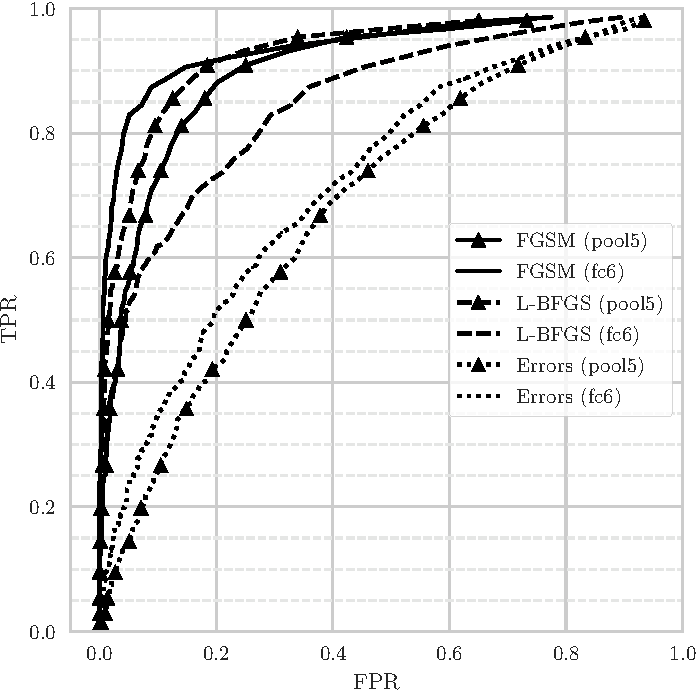
\includegraphics[width=.85\linewidth]{roc}
\caption{\gls{roc} curves of the binary classification (`prediction is right' or `prediction is wrong') for the various types of images.
The curves are obtained varying the discrimination threshold on the score assigned by the DW-kNN classifier to the class predicted by the CNN.
We only report the curves of the best performing configurations, that are \emph{fc6} with no processing, and \emph{pool5} with PCA and whitening.
Notice that when using \emph{pool5} we obtain a detection less sensible to a particular adversarial generation process.
}
\label{fig:adv:roc}
\end{figure}

In \ref{fig:adv:roc}, we report the \acrfull{roc} curves of the DW-kNN scoring approach on adversarial images and authentic errors.
The curves illustrate the performance of the proposed binary classifier when varying the threshold on the score $s(\x, f(\x))$.
%The results show that W-kNN is generally preferable when low FP rate are requested while DW-kNN is more effective when FP and TP are comparable.
As mentioned before, although \emph{fc6} performs better at detecting \gls{fgsm} adversarial examples, using \emph{pool5} activations result in a detector more robust in general.
However, we observed that higher kNN scores (which correspond to difficult L-BFGS adversarial to detect) usually reflects inter-class visual similarities that are independent from the adversarial nature of the input image (see \ref{tab:adv:bad-examples} for some examples).
The \gls{roc} curve for errors is the worst, indicating that our approach confuse correctly and incorrectly classified authentic images.
As mentioned before, the detection of authentic images incorrectly classified (errors) would be a desirable property of our approach, but it is not our main goal.

\begin{figure}
\centering
%
\begin{subfigure}[t]{0.5\linewidth}
\centering
\textbf{pool5}\\
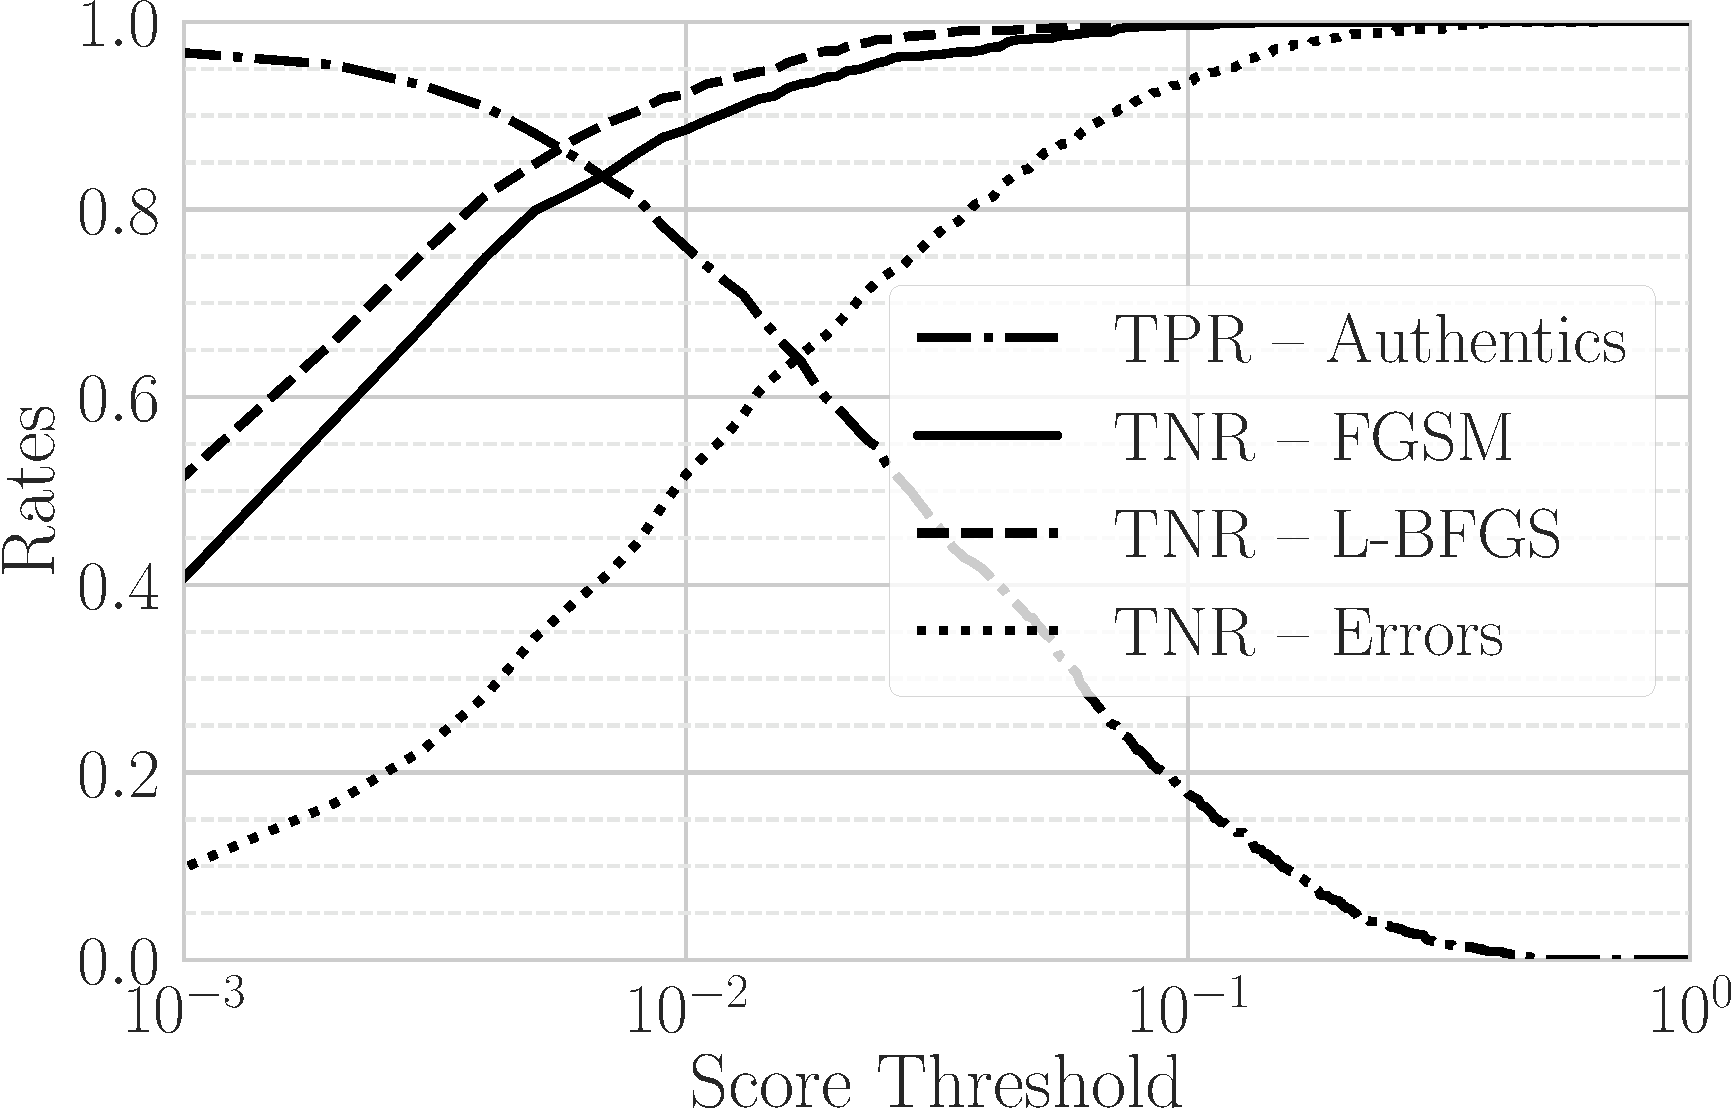
\includegraphics[width=\linewidth]{rates-pool5}%
\label{fig:adv:tpfn-dist-pool5}
\end{subfigure}%
%
\begin{subfigure}[t]{0.5\linewidth}
\centering
\textbf{fc6}\\
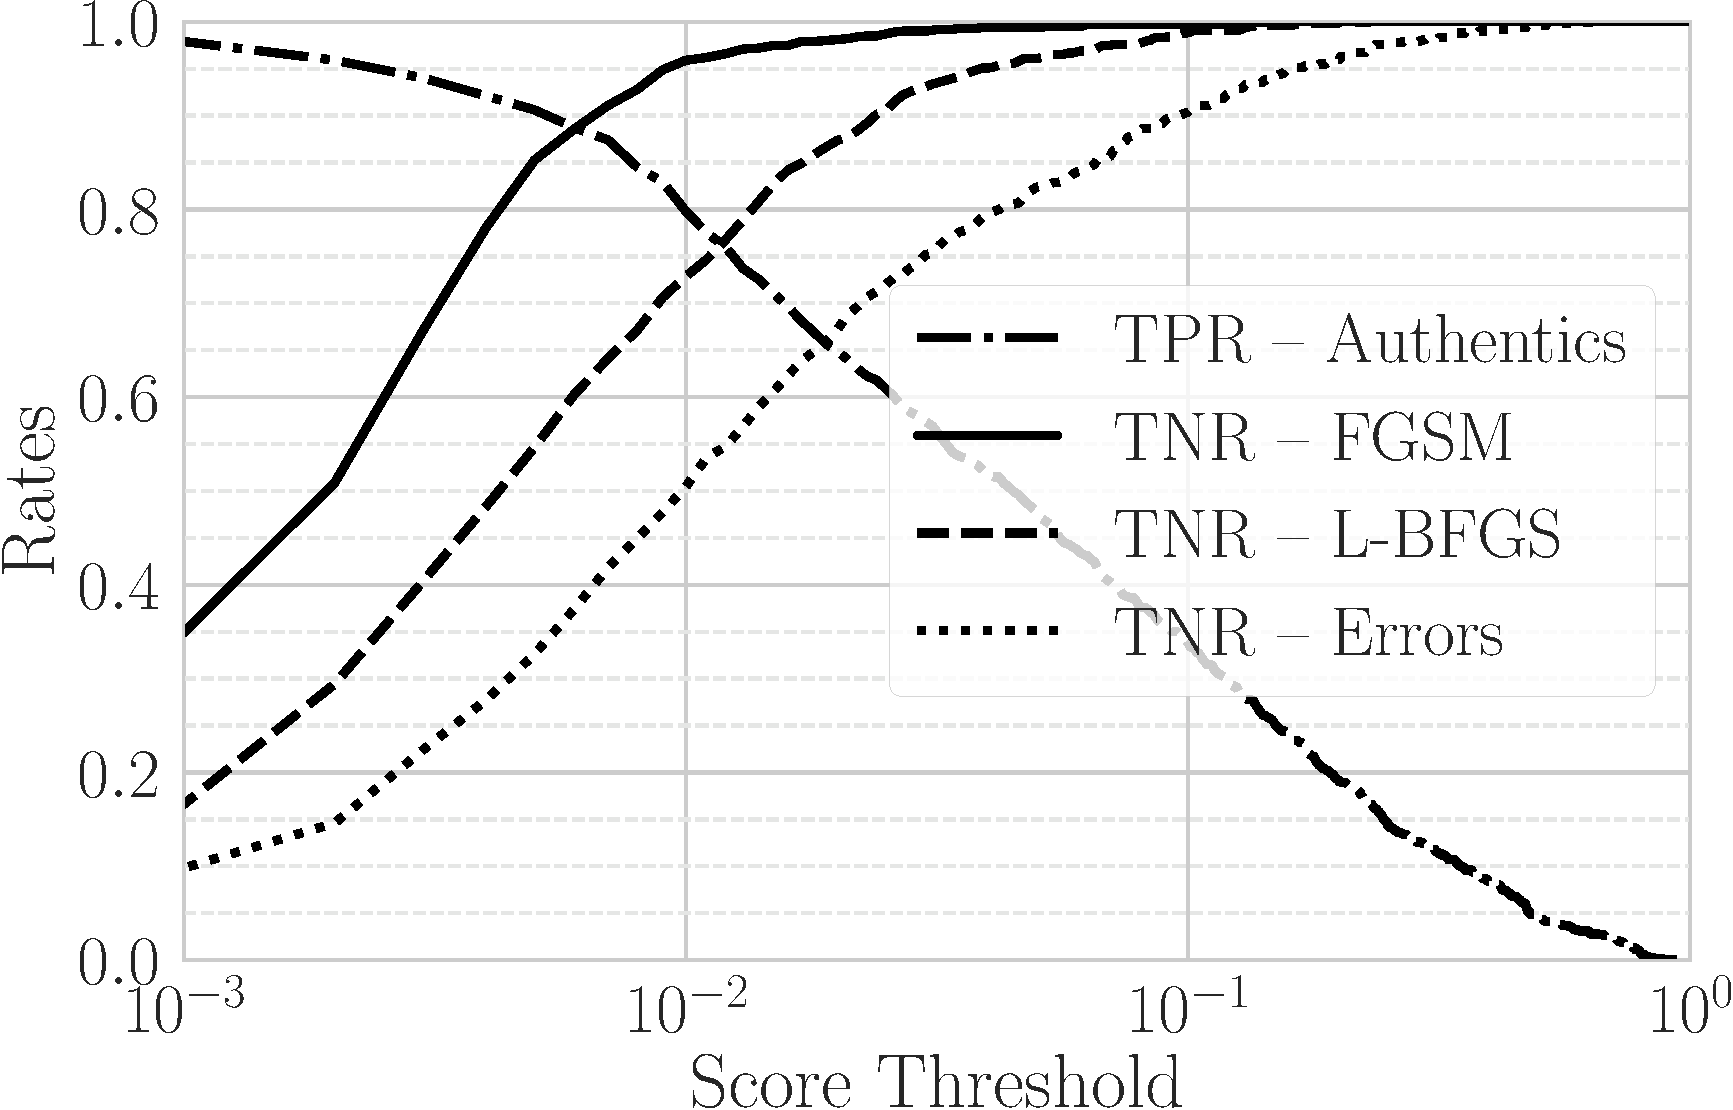
\includegraphics[width=\linewidth]{rates-fc6}%
\label{fig:adv:tpfn-dist-fc6}
\end{subfigure}%
\caption{True positive and true negative rates using as discrimination threshold between correctly and incorrectly classified images the score assigned by the DW-kNN classifier to the class predicted by the CNN.
The \emph{pool5} (on the left) and \emph{fc6} (on the right) layers have been used as features with PCA and Whitening processing.}
\label{fig:adv:tptn-distribs}
\end{figure}

Since we do not notice a prevalence of one of the three kNN weighting scheme tested, for the rest of the section, we will present results only for the DW-kNN scheme.
In \ref{fig:adv:tptn-distribs}, we report the true positive (for correctly classified authentic images) and true negative (for adversarial images and authentic errors) rates as a function of the discriminant threshold applied on the score $s(\x, f(\x))$.
Please note that for our method positive means non-adversarial.
We can easily note that using very low discrimination score values (about $0.002$), it is possible to correctly filter out more than $50\%$ of the adversarial examples created by L-BFGS and more than $40\%$ of the ones created by \gls{fgsm}, while retaining more than $98\%$ of authentic images correctly classified.
As a positive side-effect, we also discard around $10\%$ of images the \gls{dnn} would misclassify.
The low threshold values reveal that while the DW-kNN score would not be effective in classifying the images, values below $0.003$ are unlikely for authentic images.

The same results can be observer in the score densities reported in \ref{fig:adv:score-densities}, in which emerges a distinction between the score densities of adversarial images and the ones of authentic images.
Some simple statistics on those densities (such as the mean) could be computed on-line in the system hosting the model to isolate a particular source of adversarial examples, hence denying the access to the service to an attacker.

%In this paper, we focused on detecting individual adversarial examples. However, the results show that
%identifying as authentic more than $98\%$ of the images.
% \begin{table}[t]
% \small
% \centering
% \input{tab_clas}
% \caption{Accuracy of the classification using the kNN classification approach.}
% \label{tab:clas}
% \end{table}
% We also report the performance of the kNN classification approach, in which we predict the class of a given image taking the class having the maximum kNN score (see Equation \eqref{knn-classif}). Table \ref{tab:clas} shows the kNN classification accuracy for the different types of images we tested. While the kNN score helps in detecting adversarial examples, it is clear that it cannot be used to assign the correct class to adversarial examples, in particular for the images created using the FGS approach.

Finally in \ref{tab:adv:examples}, we report examples of successful detections and failures of our approach applied to the generated adversarial images. %, together with the nearest neighbor image in the kNN's labeled set and the score $s(x,f(x))$.
As anticipated, we observed that the most blatant failures (in which adversarial examples got higher scores) consist of attacks in which the target class share a strong visual similarity with the source original class -- e.g., an image of a Greater Swiss Mountain dog which is misclassified as a Bernese mountain dog.
In those difficult cases, intermediate representations of the target class are reasonable to lie around the ones of the original class in the feature space, and thus it is highly probable to erroneously obtain a confirmation of the classification of the \gls{dnn} by the kNN scoring approach.

\begin{table}
\centering
\newcommand{\imgside}{17mm}
\newcommand{\parside}{20mm}
\newcommand{\img}[1]{\parbox[c][\imgside]{\imgside}{\includegraphics[width=\imgside]{examples/#1}}}
%\newcommand{\pb}[1]{\parbox{\parside}{#1}}
\newcommand{\pb}[1]{#1}
\begin{subtable}{\linewidth}
\begin{tabularx}{\linewidth}{lcllcc}
\toprule
\textsc{Algorithm}&                            $\x'$ &                       \textsc{Actual} & \textsc{Predicted} & \textsc{1-NN} & $s$  \\
\midrule
L-BFGS   & \img{n02837789_ILSVRC2012_val_00004709_adversarial.png} & \pb{bikini, two-piece}                & pomegranate    & \parbox[c][\imgside]{\imgside}{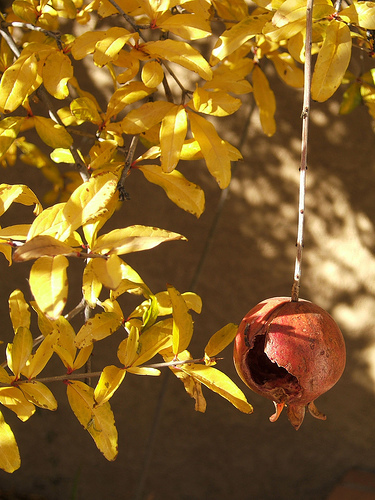
\includegraphics[width=\imgside,trim={0 1cm 0 3.5cm},clip]{examples/n07768694_863.JPEG}}   & 0.01 \\ \midrule
FGSM     & \img{n02892767_ILSVRC2012_val_00004599_adversarial.png} & \pb{brassiere, bra, bandeau}          & Chihuahua	    & \img{n02085620_10227.JPEG} & 0.01 \\ \midrule
FGSM     & \img{n04086273_ILSVRC2012_val_00011273_adversarial.png} & \pb{revolver, six-gun, six-shooter}   & mousetrap      & \img{n03794056_4688.JPEG}  & 0.00 \\ \midrule
L-BFGS   & \img{n02749479_ILSVRC2012_val_00039278_adversarial.png} & \pb{assault rifle, assault gun}       & Border terrier & \img{n02093754_3.JPEG}     & 0.00 \\
\bottomrule
\end{tabularx}
\caption{Examples of good detections of adversarial images with content that might be filtered. Low scores reflect a low confidence of image authenticity.\\[2ex]}
\label{tab:adv:good-examples}
\end{subtable}
\begin{subtable}{\linewidth}
\begin{tabularx}{\linewidth}{lclXcc}
\toprule
\textsc{Algorithm}&                            $\x'$ &                       \textsc{Actual} & \textsc{Predicted} & \textsc{1-NN} & $s$  \\
\midrule
FGSM     & \img{n03017168_ILSVRC2012_val_00041177_adversarial.png} & \pb{chime, bell, gong}      & barometer                                  &  \img{n02794156_12351.JPEG}  & 0.13 \\ \midrule
%L-BFGS   & \img{n02110806_ILSVRC2012_val_00025245_adversarial.png} & basenji                     & \pb{Arctic fox, white fox, Alopex lagopus} &  \img{n02120079_34796.JPEG}  & 0.13 \\ \midrule
L-BFGS   & \img{n02110806_ILSVRC2012_val_00025245_adversarial.png} & basenji                     & Arctic fox, white fox                      &  \img{n02120079_34796.JPEG}  & 0.13 \\ \midrule
FGSM     & \img{n02107574_ILSVRC2012_val_00033603_adversarial.png} & Greater Swiss Mountain dog  & Bernese mountain dog                       &  \img{n02107683_3087.JPEG}  & 0.11 \\ \midrule
FGSM     & \img{n03594945_ILSVRC2012_val_00041895_adversarial.png} & jeep, landrover             & pickup, pickup truck                       &  \img{n03930630_9160.JPEG}  & 0.11 \\
\bottomrule
\end{tabularx}
\caption{Examples of bad detections of adversarial images. Those are adversarial images for which our approach wrongly assigned a high score. However, this is mainly due to the visual similarity between the actual and fooled class.}
\label{tab:adv:bad-examples}
\end{subtable}

\caption{Examples of detections of adversarial images obtained by our best approach (\emph{pool5}+PCA+DW-kNN).
From left to right, columns respectively report: the adversarial generation algorithm, the generated adversarial image, its original class, the class predicted by the \gls{dnn}, the nearest neighbor image (in terms of L2 distance between average-pooled \emph{pool5} activations) belonging to the predicted class, and the DW-kNN score $s$ for the predicted class.
A low score indicates that the adversarial is correctly detected (\subref{tab:adv:good-examples}) while a high score means that our approach is wrongly confident about the prediction of the CNN (\subref{tab:adv:bad-examples}).
The results show that high scoring adversarial examples often share some common visual aspects and semantic with the predicted (adversarial) class, resulting in a more challenging detection.
}
\label{tab:adv:examples}
\end{table}

\begin{figure}
\centering%
%
\begin{subfigure}[t]{0.5\linewidth}%
\centering
\textbf{pool5}\\
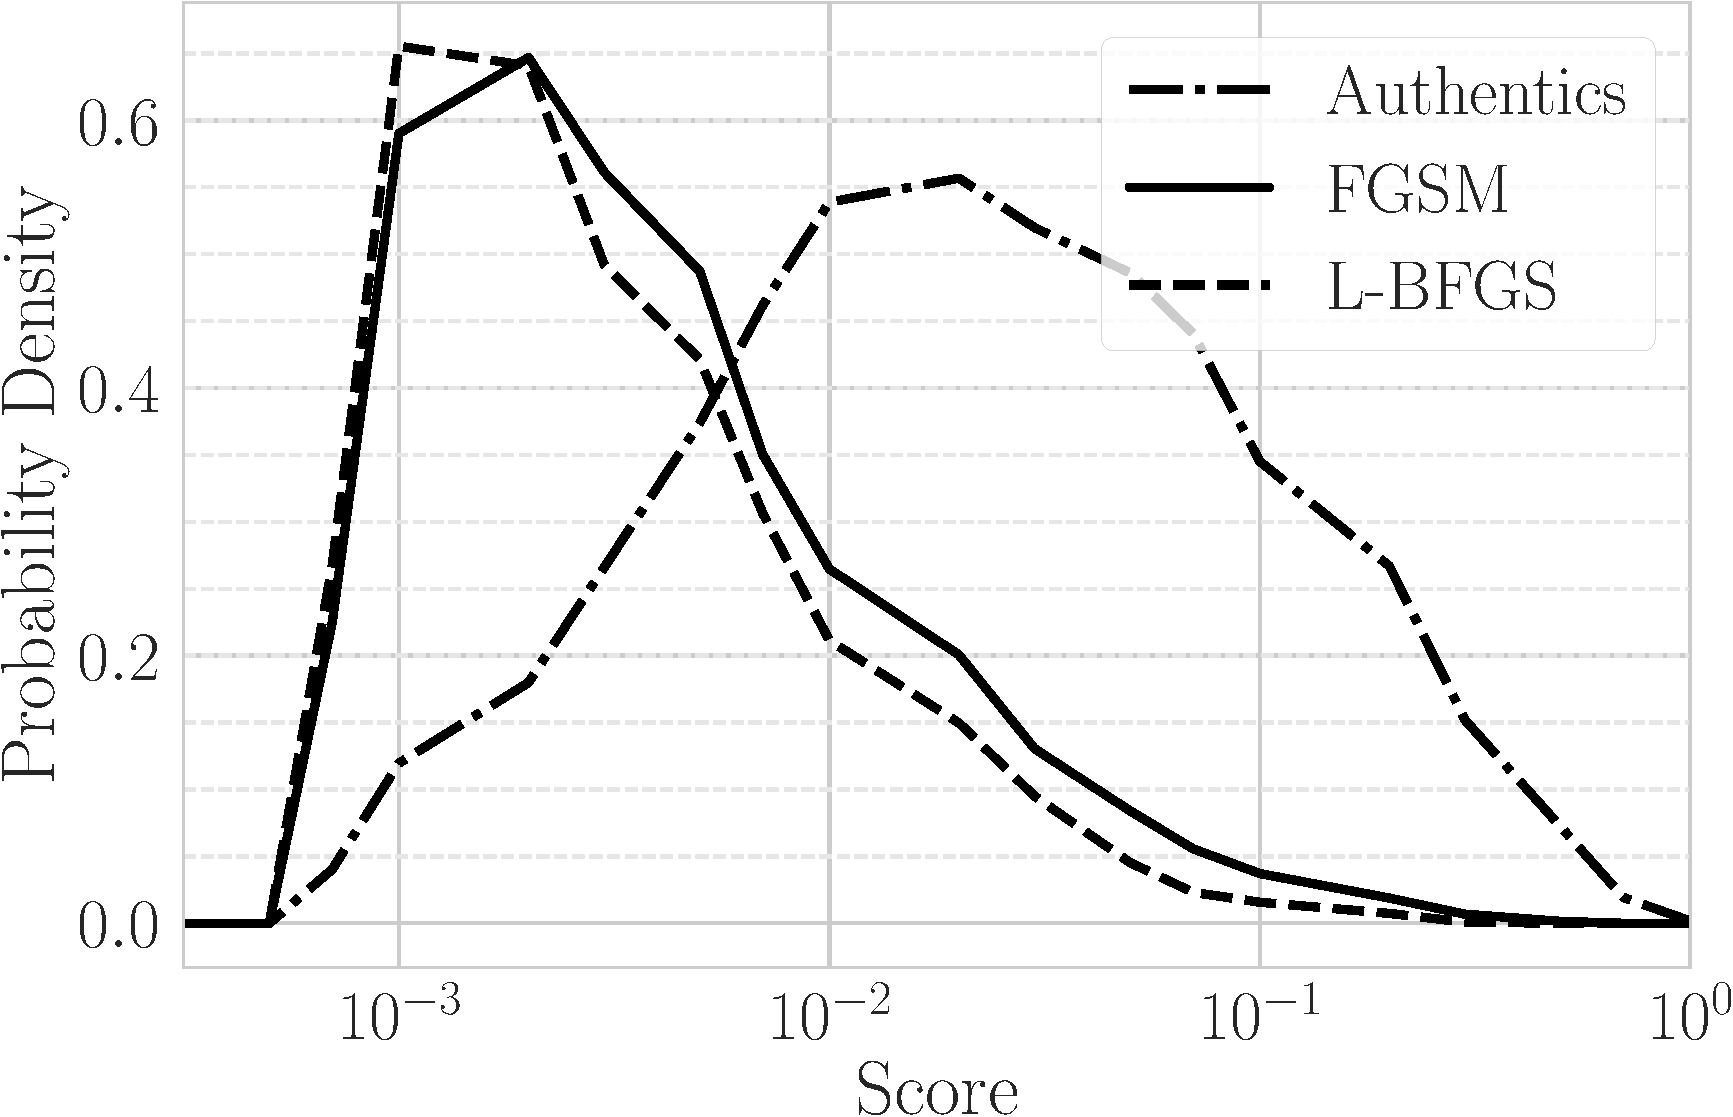
\includegraphics[width=\linewidth]{distrib-pool5}%
\label{fig:adv:score-density-pool5}%
\end{subfigure}%
%
\begin{subfigure}[t]{0.5\linewidth}%
\centering
\textbf{fc6}\\
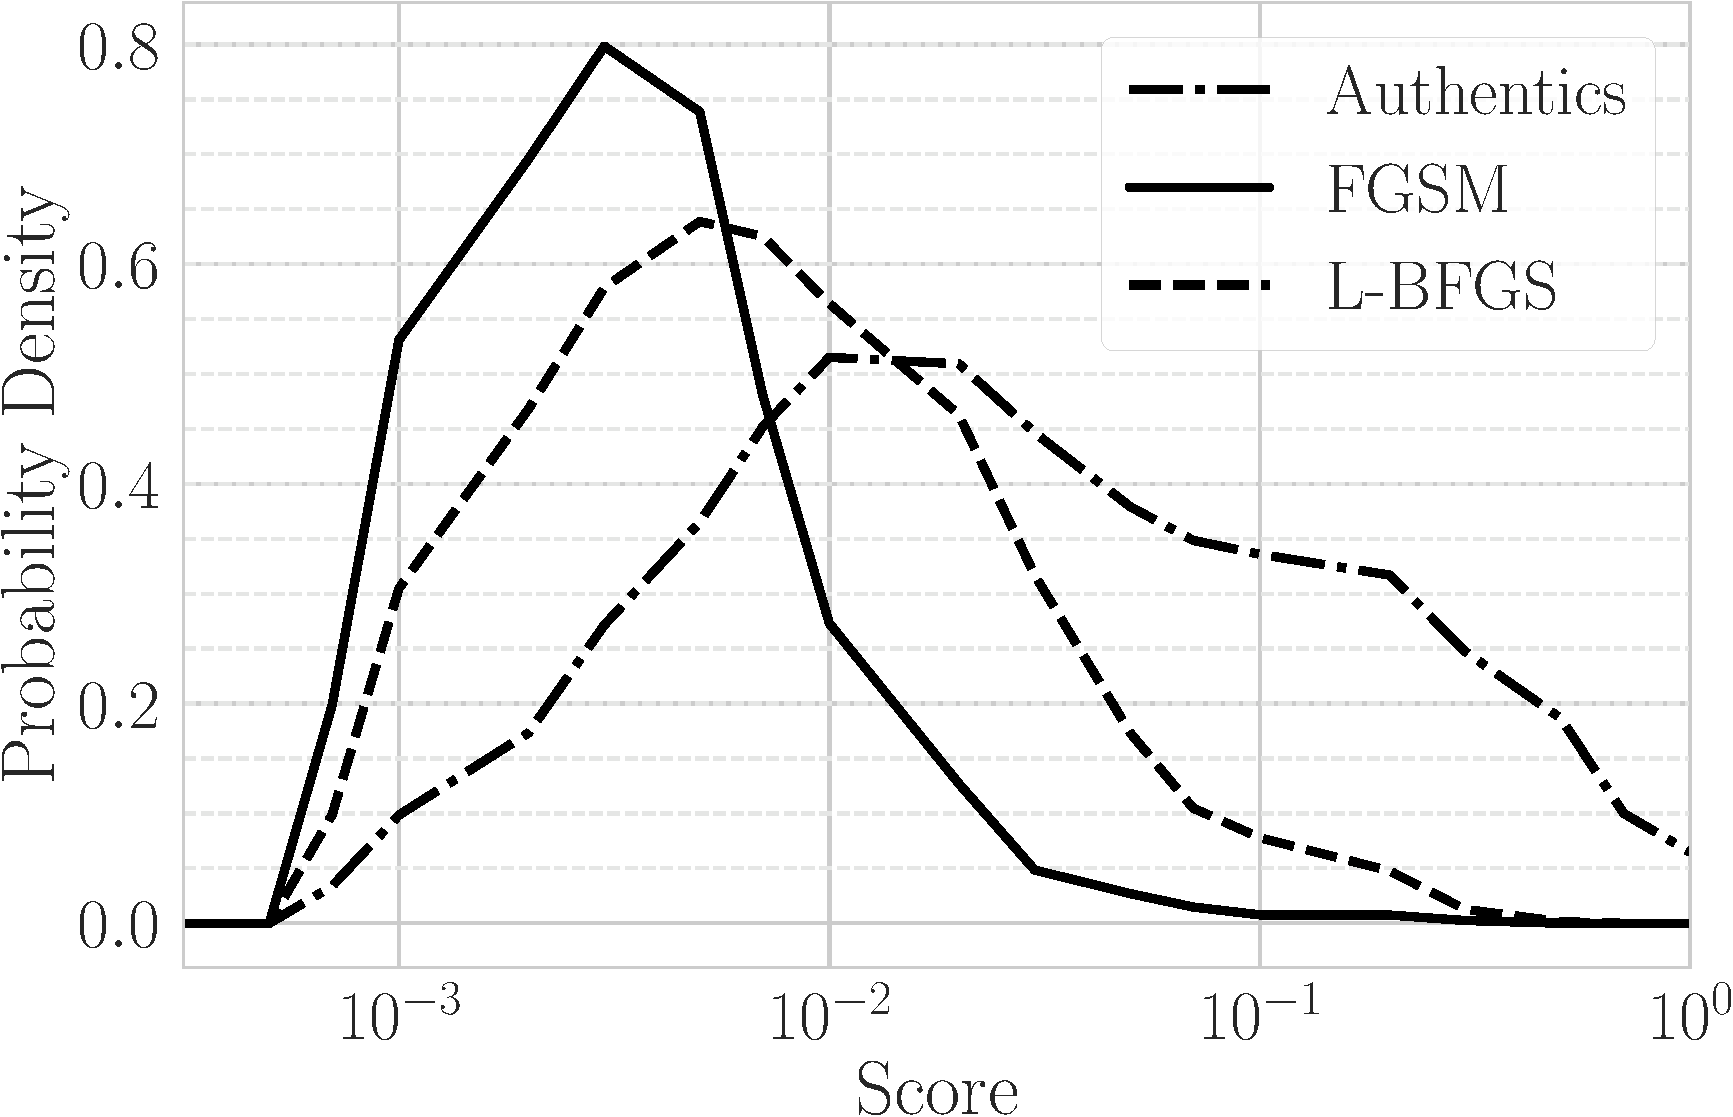
\includegraphics[width=\linewidth]{distrib-fc6}%
\label{fig:adv:score-density-fc6}%
\end{subfigure}%
%
\caption{Density of the DW-kNN scores for both adversarial and authentic images.
We report densities of scores using \emph{pool5} (on the left) and \emph{fc6} (on the right) as feature and PCA+Whitening as processing.}
\label{fig:adv:score-densities}
\end{figure}

\subsection{\emph{InceptionV3} Network on NIPS 2017 Adversarial Competition Dataset}
\label{subsec:adv:inception}

In the following experiments, we applied our detection algorithm to a more recent model, that is InceptionV3~\cite{szegedy2016rethinking}, which has been used as baseline classifier in the NIPS 2017 Adversarial Attacks and Defenses Kaggle Competitions~\cite{kurakin2018adversarial}.
Thus, instead of selecting random images from the \gls{ilsvrc}'12 validation set, we used the DEV images set released for the competition.
The DEV set is composed of $1,000$ images that are not part of the ImageNet dataset, yet they have been manually labelled using the \gls{ilsvrc}'12 labels.

We followed the same methodology as in \ref{subsec:adv:overfeat}: we set apart from the DEV set the images that were incorrectly classified by InceptionV3; for the remaining images, we applied four different perturbation schemes (we generated the last two adversarial perturbations using the \emph{cleverhans} library~\cite{papernot2018cleverhans}):

%\SetLabelAlign{parright}{\parbox[t]{\labelwidth}{\bfseries \itshape \raggedleft#1}}
\begin{description}%[leftmargin=!,labelwidth=2.5cm, align=parright]
  \item[noop] the image is unchanged (authentic);
  \item[random\_noise] the image is perturbed adding random gaussian noise in the interval $[-16, +16]$;
  \item[fgsm] the image is perturbed with FGSM (see \ref{sec:adv:algos}) with $\epsilon = 16$ choosing a random target class;
  % TODO add I-FGSM from workshop paper
  \item[i-fgsm] the image is perturbed with 20 iterations of FGSM algorithm with $\epsilon = 1$; the target class is randomly chosen and kept fixed for all the iterations; the total perturbation is clipped to be in the interval $[-16, +16]$.
\end{description}

Since \textbf{\emph{random\_noise}} images are not meant to directly attack the classifier, we considered them authentic images. % together with the untouched images (\textbf{\emph{noop}}).
As in \ref{subsec:adv:overfeat}, we removed failed adversarial images produced by \textbf{\emph{fgsm}} or \textbf{\emph{i-fgsm}}, i.e., adversarial perturbed images for which the prediction of the network has not changed.
We also left out images produced by \textbf{\emph{random\_noise}} that are misclassified by the network, in order not to tamper the analysis of our adversarial detection approach with errors committed naturally by the classifier.
From this procedure, we obtained a test set comprising correctly classified authentic images and successfully generated adversarial images.

%For each image, we computed a score with our method for each proposed kNN scoring schemes (see \ref{sec:adv:detection}).
We performed a thorough exploration on the choice of the intermediate activation to be extracted from the InceptionV3 model.
We extracted convolutional features after each inception module, and we obtained compact representations applying global average pooling.
We also performed PCA dimensionality reduction to 256 components, since it had been proved beneficial for convolutional features in previous experiments (see \ref{subsec:adv:overfeat}).

% \subsubsection{Results}
% \label{subsec:adv:i3-results}

\begin{table}
\renewcommand{\tabcolsep}{3pt}
\newcolumntype{R}{>{\raggedleft\arraybackslash}X}%
\newcolumntype{C}{>{\centering\sloppy\arraybackslash}X}%
\begin{tabularx}{\linewidth}{Xcccccccccccc}
\toprule
                 & \multicolumn{4}{c}{\textsc{kNN}} & \multicolumn{4}{c}{\textsc{W-kNN}} & \multicolumn{4}{c}{\textsc{DW-kNN}} \\
                   \cmidrule(lr){2-5}                 \cmidrule(lr){6-9}                   \cmidrule(lr){10-13}
\textsc{Layer}   &  \multicolumn{1}{c}{\footnotesize\textbf{FGSM}} &  \multicolumn{1}{c}{\sloppy\footnotesize\textbf{I-FGSM}} &  \multicolumn{1}{c}{\footnotesize\textbf{Aggr.}} &  \multicolumn{1}{c}{\footnotesize\textbf{Err.}}
                 &  \multicolumn{1}{c}{\footnotesize\textbf{FGSM}} &  \multicolumn{1}{c}{\sloppy\footnotesize\textbf{I-FGSM}} &  \multicolumn{1}{c}{\footnotesize\textbf{Aggr.}} &  \multicolumn{1}{c}{\footnotesize\textbf{Err.}}
                 &  \multicolumn{1}{c}{\footnotesize\textbf{FGSM}} &  \multicolumn{1}{c}{\sloppy\footnotesize\textbf{I-FGSM}} &  \multicolumn{1}{c}{\footnotesize\textbf{Aggr.}} &  \multicolumn{1}{c}{\footnotesize\textbf{Err.}} \\
\midrule
maxpool\_5a\_3x3 &          50.1 &          51.9 &          51.1 &          31.1 &          58.2 &          60.8 &          59.7 &          45.6 &          58.3 &          60.9 &          59.8 &          45.7 \\
mixed\_5b        &          53.0 &          54.4 &          53.8 &          35.4 &          59.5 &          63.0 &          61.5 &          49.1 &          59.5 &          63.0 &          61.5 &          49.1 \\
mixed\_5c        &          56.6 &          58.4 &          57.6 &          41.2 &          62.2 &          66.9 &          64.9 &          54.6 &          62.2 &          66.9 &          64.9 &          54.5 \\
mixed\_5d        &          57.6 &          59.8 &          58.9 &          43.2 &          63.8 &          68.7 &          66.6 &          57.5 &          63.8 &          68.8 &          66.6 &          57.8 \\
mixed\_6a        &          62.6 &          65.7 &          64.4 &          51.5 &          68.7 &          74.4 &          72.0 &          61.7 &          68.8 &          74.4 &          72.0 &          62.7 \\
mixed\_6b        &          62.3 &          72.7 &          68.2 &          52.8 &          67.8 &          79.9 &          74.7 &          63.1 &          68.0 &          80.0 &          74.8 &          64.0 \\
mixed\_6c        &          70.7 &          80.6 &          76.3 &          60.5 &          71.0 &          82.5 &          77.6 &          68.2 &          71.4 &          82.3 &          77.6 &          69.2 \\
mixed\_6d        &          70.9 & \textbf{83.0} & \textbf{77.8} &          64.5 &          71.7 & \textbf{84.6} & \textbf{79.1} &          69.4 &          71.6 & \textbf{85.0} & \textbf{79.2} &          69.5 \\
mixed\_6e        &          72.5 &          74.2 &          73.5 &          71.3 &          74.3 &          75.6 &          75.1 &          72.1 &          72.8 &          75.5 &          74.4 &          72.6 \\
mixed\_7a        &          73.0 &          77.2 &          75.4 &          71.4 & \textbf{75.5} &          78.4 &          77.2 &          75.0 &          74.4 &          78.3 &          76.7 &          73.1 \\
mixed\_7b        &          73.7 &          70.5 &          71.9 &          75.2 &          75.1 &          71.3 &          72.9 &          76.5 &          74.4 &          71.4 &          72.7 &          76.1 \\
mixed\_7c        & \textbf{74.0} &          52.0 &          61.5 & \textbf{78.5} &          74.4 &          52.3 &          61.9 & \textbf{80.5} & \textbf{74.5} &          52.8 &          62.2 & \textbf{79.0} \\
\bottomrule
\end{tabularx}
\caption{\Gls{eer} detection accuracies for each (scoring scheme, layer) combination.
The accuracies are computed putting together each subset (\textbf{\emph{fgsm}} or \textbf{\emph{i-fgsm}}) with the set authentic images.
The \textbf{Aggr.} column reports a weighted mean of the accuracies on all subsets.
The \textbf{Errors} column report the recover accuracy fo natural (non-adversarial) errors committed by the network.}
\label{tab:adv:i3-eer}
\end{table}

In \ref{tab:adv:i3-eer}, we report the \gls{eer} accuracy obtained on the test set for each layer used to extract deep features and considering each kNN scoring scheme.
We noticed that the effectiveness of the detection increases adopting higher-level layers of the network, until we reach the fooled layers, where the accuracy drops.
The first layers of the network produce activations not representative enough of class-level semantic concepts, while the last layers are steered by the adversarial crafting algorithms.
This behavior suggests that current adversarial crafting algorithms do not steer all the internal semantic representations inside the network.
Thus, we are able to find a good compromise between representativeness and robustness to adversarial manipulation.

In \ref{fig:adv:i3-distr}, we report the true positive (correctly classified authentic images predicted as non-adversarial) and true negatives (adversarial images and authentic errors detected by our method) rates distributions as a function of the discriminant threshold applied on the score (positive means non-adversarial).
Although lower-level features seem not to affect the detection of less perturbed images (i.e., \gls{fgsm}), we noticed that they play a fundamental role to detect strong adversarial such as \textbf{\emph{i-fgsm}} (\ref{fig:adv:i3-distr} on the left).
This is reasonable given that the stronger attack we analyzed, i.e., \textbf{\emph{i-fgsm}}, tends to affect multiple layers in the last stage of the network, thus being better detected using more internal lower-level activations, while FGSM can be easily detected using higher-level layers.

Weighted scoring schemes (W-kNN and DW-kNN) seem to outperform the naive kNN scheme, specially when combined with low level features (see \ref{fig:adv:i3-eer}).
Overall, the best performance is obtained using the \textbf{\emph{mixed\_6d}} layer and the DW-kNN scheme, reaching a mean EER accuracy of 79.2\%.
Moreover, our method is able to recover around 80\% of natural errors committed by the network. This rate is considerably higher than the ones presented in \ref{tab:adv:eer} due to the presence of \textbf{\emph{random\_noise}} images, that produced lots of easily recoverable misclassifications.


\begin{figure}
\centering%
%
\begin{subfigure}[t]{0.5\linewidth}%
\centering
\textbf{mixed\_6d}\\
\includegraphics[width=\linewidth]{score_distribution_mixed_6d_dwknn}%
\label{fig:adv:score-density-mixed_6e}%
\end{subfigure}%
%
\begin{subfigure}[t]{0.5\linewidth}%
\centering
\textbf{mixed\_7a}\\
\includegraphics[width=\linewidth]{score_distribution_mixed_7a_dwknn}%
\label{fig:adv:score-density-mixed_7a}%
\end{subfigure}%
%
\caption{True positive and false positive rates when varying the score threshold. The scores are computed using \textbf{\emph{mixed\_6d}} (on the left) and \textbf{\emph{mixed\_7a}} (on the right) of the InceptionV3 classifier.
DW-kNN scoring scheme was selected for both.}
\label{fig:adv:i3-distr}
\end{figure}

\begin{figure}
\centering
{\includegraphics[width=\columnwidth]{incepv3_eer-acc}}
\caption{ The Equal Error Rate accuracy obtained on the NIPS DEV set using different intermediate activations of the InceptionV3 as deep features.
Note that the effectiveness of the detection gets better when using deeper representations, and rapidly decreases when we reach the fooled layers at the end of the network.}
\label{fig:adv:i3-eer}
\end{figure}


\section{Conclusions and Future Work}
\label{sec:adv:conclusions}

In this chapter, we presented an approach to detect adversarial examples crafted for fooling deep neural network classifiers.
The overall goal is filtering out malicious images.
To perform the detection, we relied on activations of neurons in hidden layers in order to detect adversarials.
In particular, we inspect the activations of intermediate layers for both adversarial and authentic inputs, and we defined an authenticity confidence score based on kNN similarity searching among the images used for training.
Experiments on the two most cited adversarial generation techniques (L-BFGS and \gls{fgsm}) on the very same neural network used in the original papers (i.e., Overfeat, InceptionV3) have been carried out.
In the experiments, we considered various kNN score functions and hidden layers.

%The results show that we were able to filter out roughly $85\%$ of adversarial images when looking to lower level activations (such as \emph{pool5}).
%Specifically, results shown that adversarials generated with L-BFGS are particularly difficult to detect.

When attacking the OverFeat model, the proposed approach allows to filter about $80\%$ of adversarial examples retaining more than $90\%$ of the correctly classified authentic images (see \ref{fig:adv:tptn-distribs}).
We also showed that the probability density function of our authenticity confidence obtained over adversarial examples significantly differs from the one obtained for authentic images.
%We showed that lower-level activations (such as \emph{pool5} with global average pooling) increase the detection performance with respect to the higher-level ones.
Moreover, some examples are suggesting that hard adversarial examples are the ones for which actual and target classes are similar or have similar visual patterns. %there are same visual patterns in both classes.

We also tested our method on the InceptionV3 \gls{dnn}, generating adversarial images from the NIPS 2017 Adversarial Attacks and Defenses Kaggle Competitions.
Using this dataset, we performed a thorough analysis of the detectability of adversarial exampels when varying the internal layer extracted from the \gls{dnn}.
Best results were obtained using layer \emph{\textbf{mixed\_6d}} with an overall EER Accuracy of $80\%$, confirming the effectiveness of our approach and its general applicability to deep neural network classifiers.
Future work may test the detection scheme under a more stringent threat model, in which the attacker is aware of the detection scheme used.
The comparison of multiple layers for the detection performed in this study suggested that current adversarial crafting algorithms do not steer all the internal semantic representations inside the network, but focus on the last layers.
Given these considerations, possible future work may also improve the presented detection scheme by relying on multiple intermediate layers, thus increasing the difficulty for a generation algorithm to craft adversarial images able to control multiple activations at once.

\cleardoublepage
\phantomsection
\addcontentsline{toc}{chapter}{\bibname}
\small
\bibliographystyle{plainnat}
\bibliography{thesis}

\end{document}
